\documentclass{article}
\usepackage[mathletters]{ucs}
\usepackage[utf8x]{inputenc}
\usepackage{amssymb}
\usepackage{amsmath}
\usepackage[usenames]{color}
\usepackage{hyperref}
\usepackage{wasysym}
\usepackage{graphicx}
\usepackage[normalem]{ulem}
\usepackage{enumerate}

\usepackage{listings}

\lstset{ 
basicstyle=\footnotesize,       % the size of the fonts that are used for the code
showspaces=false,               % show spaces adding particular underscores
showstringspaces=false,         % underline spaces within strings
showtabs=false,                 % show tabs within strings adding particular underscores
frame=single,                   % adds a frame around the code
tabsize=2,                      % sets default tabsize to 2 spaces
breaklines=true,                % sets automatic line breaking
breakatwhitespace=false,        % sets if automatic breaks should only happen at whitespace
}


\title{ToolWearInspection}
\date{dinsdag 08 december 2020}
\author{}

\begin{document}

\maketitle

		\section{Camera setup}

Created zaterdag 24 oktober 2020



Tests of the setup: 

\begin{itemize}
\item 3D printing the tool holder
\item 3D printing a easy way of photographing many tools in an easy way
\end{itemize}




Parts of the setup:

\begin{enumerate}[1]
\item
	\begin{enumerate}[a]
	\item 3-4 led lights/strips separately controllable to light from different angles
	\item with or without extra light on top
	\end{enumerate}
\item Wheel with tool mount
	\begin{enumerate}[a]
	\item 3D model creation of mount system
	\item creating wheel to be accurate
	\item controlling stepper motor to turn just enough to put the next tool in front of the camera
	\end{enumerate}
\item Camera mount
	\begin{enumerate}[a]
	\item Design to let the camera view different angles
	\item watch out for lighting
	\end{enumerate}
\end{enumerate}





		\section{Camera mount}

Created Wednesday 28 October 2020



In this page the camera mount will be discussed along the design process of the setup



\begin{enumerate}[1]
\item Holder 
\item Wheel holder
\end{enumerate}

		\section{First Camera Mount}

Created Wednesday 28 October 2020



The printing process can be seen in the next picture:

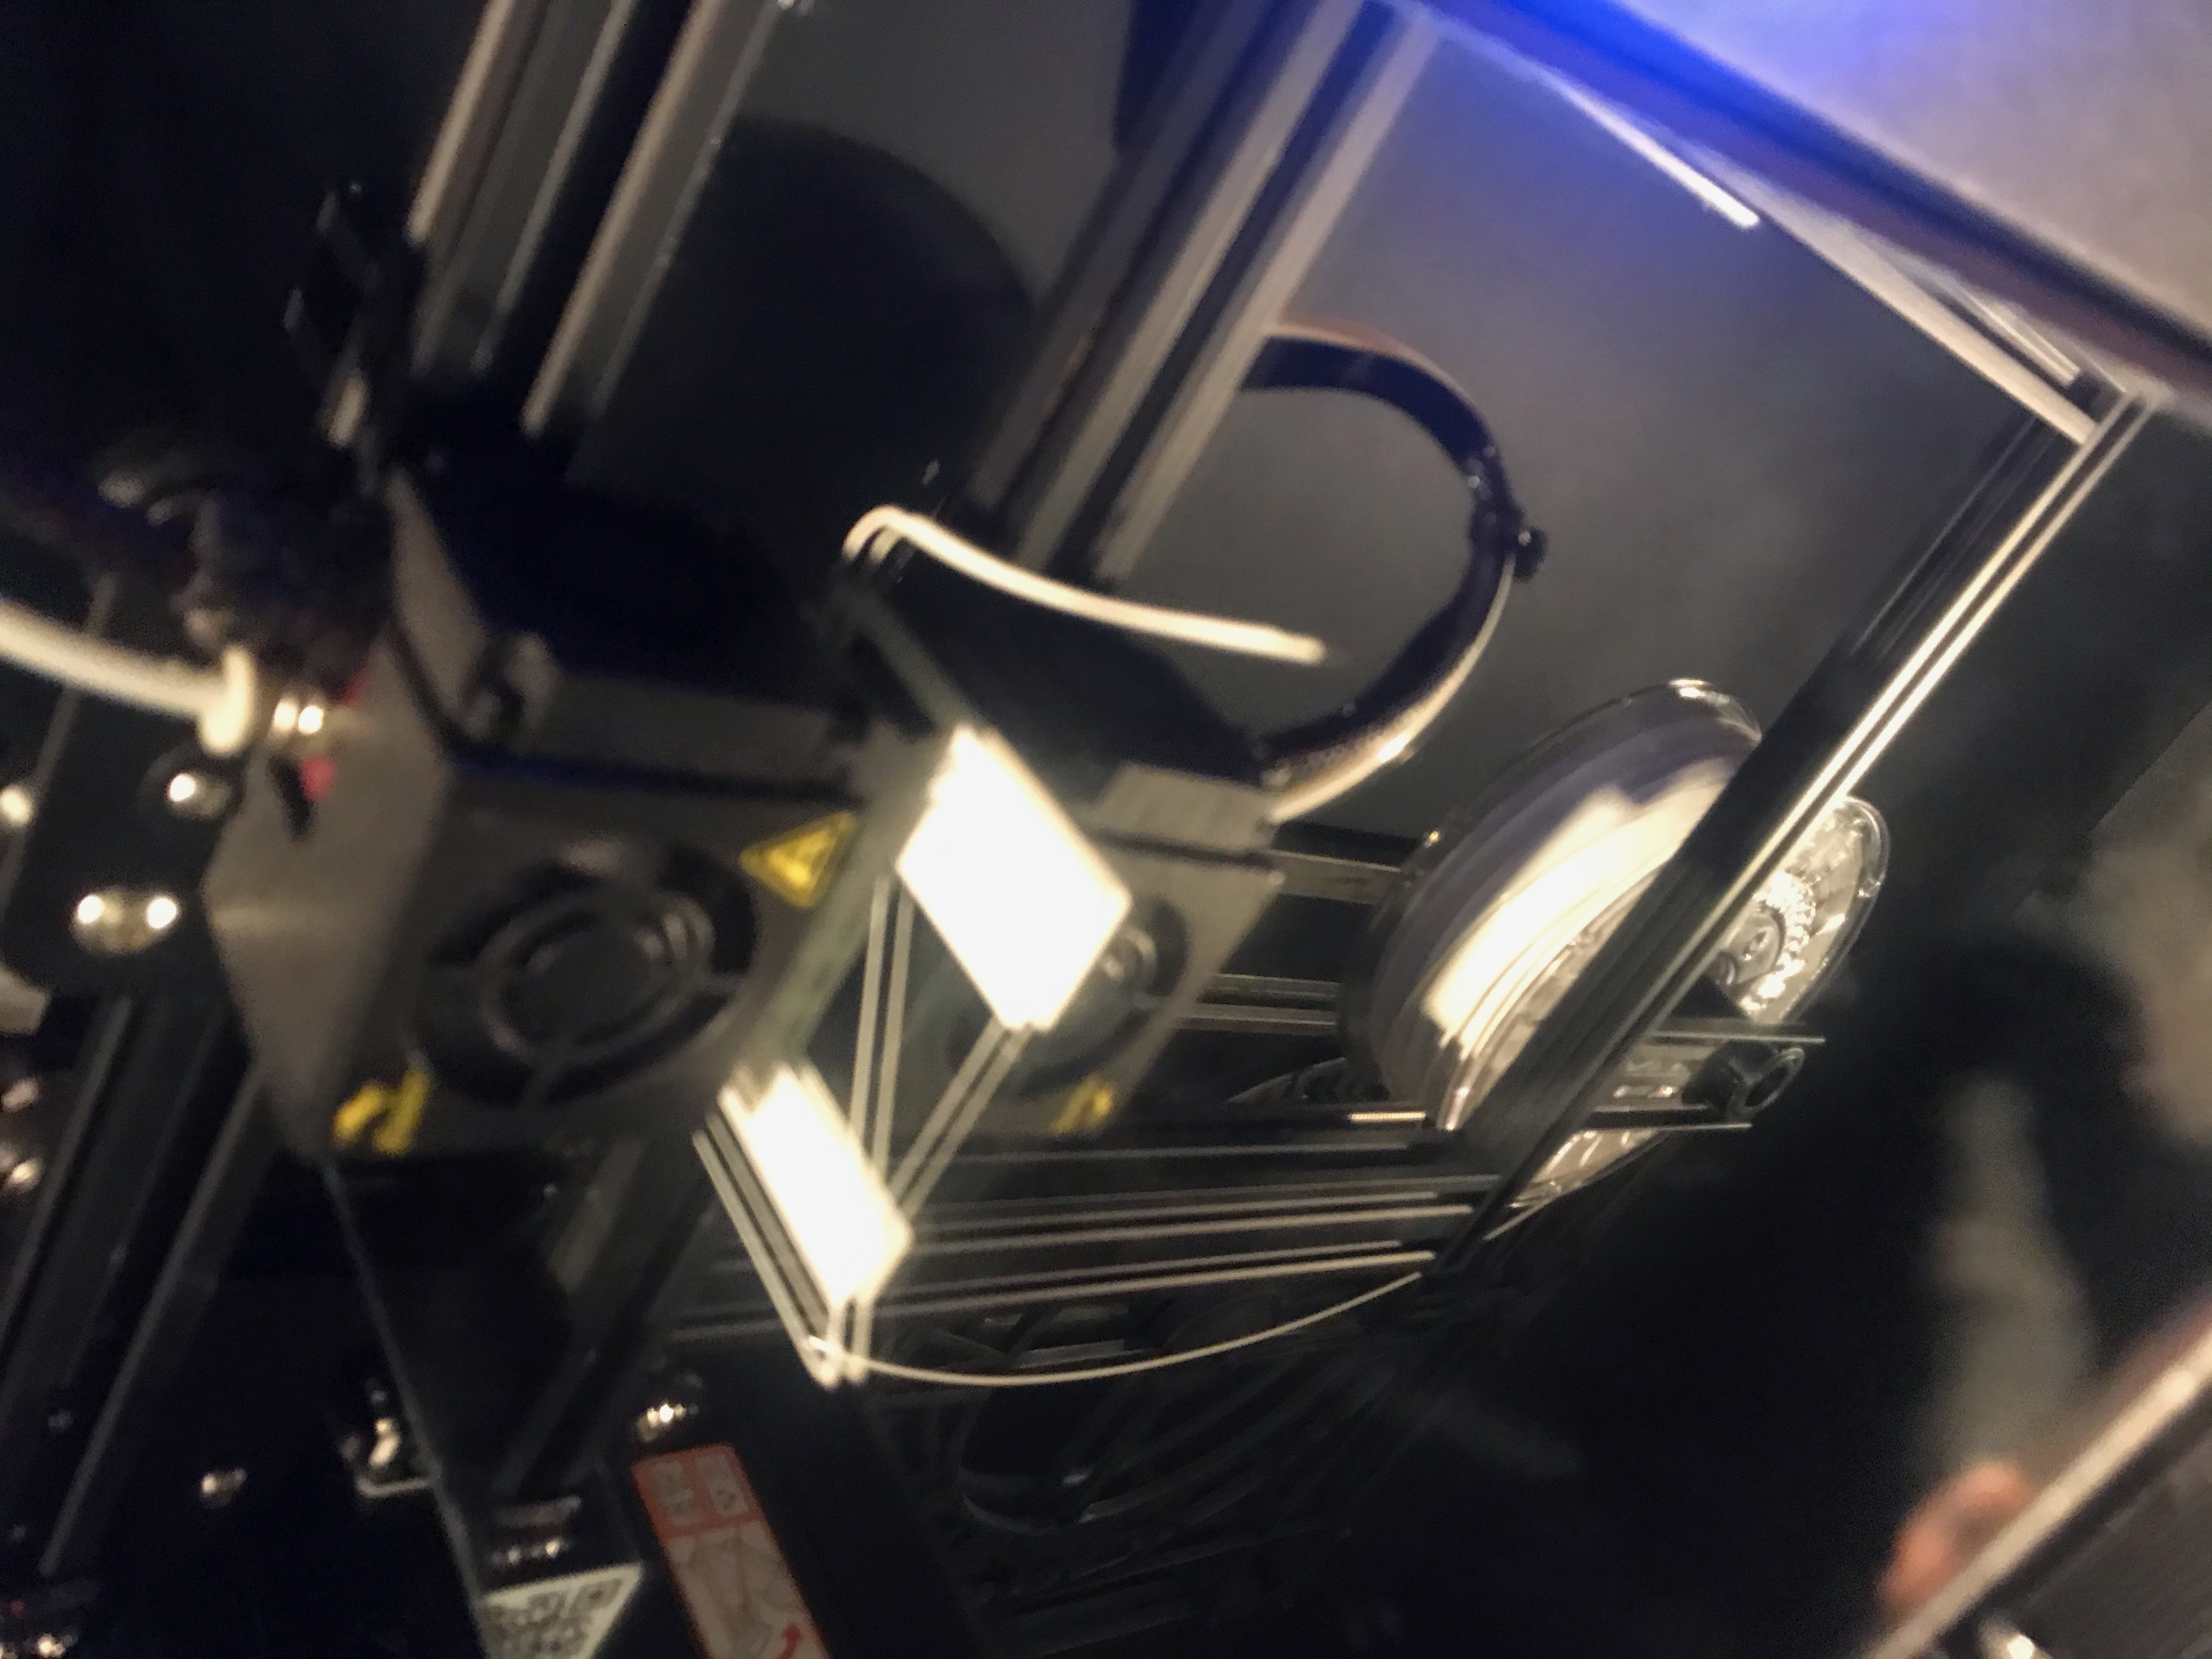
\includegraphics[height=3.125000in, keepaspectratio=true]{./ZimFiles_files/Camera_setup/Camera_mount/First_Camera_Mount/3D_print_houder.jpeg}



Here PLA is used to print on a temperature of 200 degrees Celcius, on a heated bed of 60 degree Celcius. This is a holder which should support the camera while keeping the tool on the tool holder in place. The result wasn't good due to the print not sticking enough to the printing bed, no other test print was made. There will be another mount designed further in the process when the Desk Lamp Test.



The full setup can be seen in the following picture: Here the 3D printed plate goes under the postits to get consistent placement of the tool to the camera. 

\includegraphics[height=3.125000in, keepaspectratio=true]{./ZimFiles_files/Camera_setup/Camera_mount/First_Camera_Mount/eerste_setup_andere_richting.jpeg}




		\section{Wheel Camera Mount}

Created woensdag 11 november 2020



For the wheel, the camera is used on a piece of wood in the default stand. This must be changed to a more fixed setup in order to create stable results


		\section{Light}

Created zaterdag 24 oktober 2020



Different light setups:

\begin{enumerate}[1]
\item Desk Lamp
\item white led strips (long) 
\item  led strip (single led)
\item Color changeable led strip (multiple combined in a matrix)
\item top light (white or colored)
\end{enumerate}







		\section{Adressable Color Changeable Led Strip}

Created Wednesday 28 October 2020



A third option of lighting is playing with the colors of the light. to archieve this a setup will be created with a single adressable light strip where the color and led can be freely chosen. 



To assign a color which works best; a study is made to find the wavelengths where the light reflects most on the used materials of the tool. This can be found in  Light Reflection


		\section{Desk Lamp Test}

Created Wednesday 28 October 2020



First test using following setup:



\includegraphics[width=4.166667in, keepaspectratio=true]{./ZimFiles_files/Camera_setup/Light/Desk_Lamp_Test/eerste_setup_andere_richting.jpeg}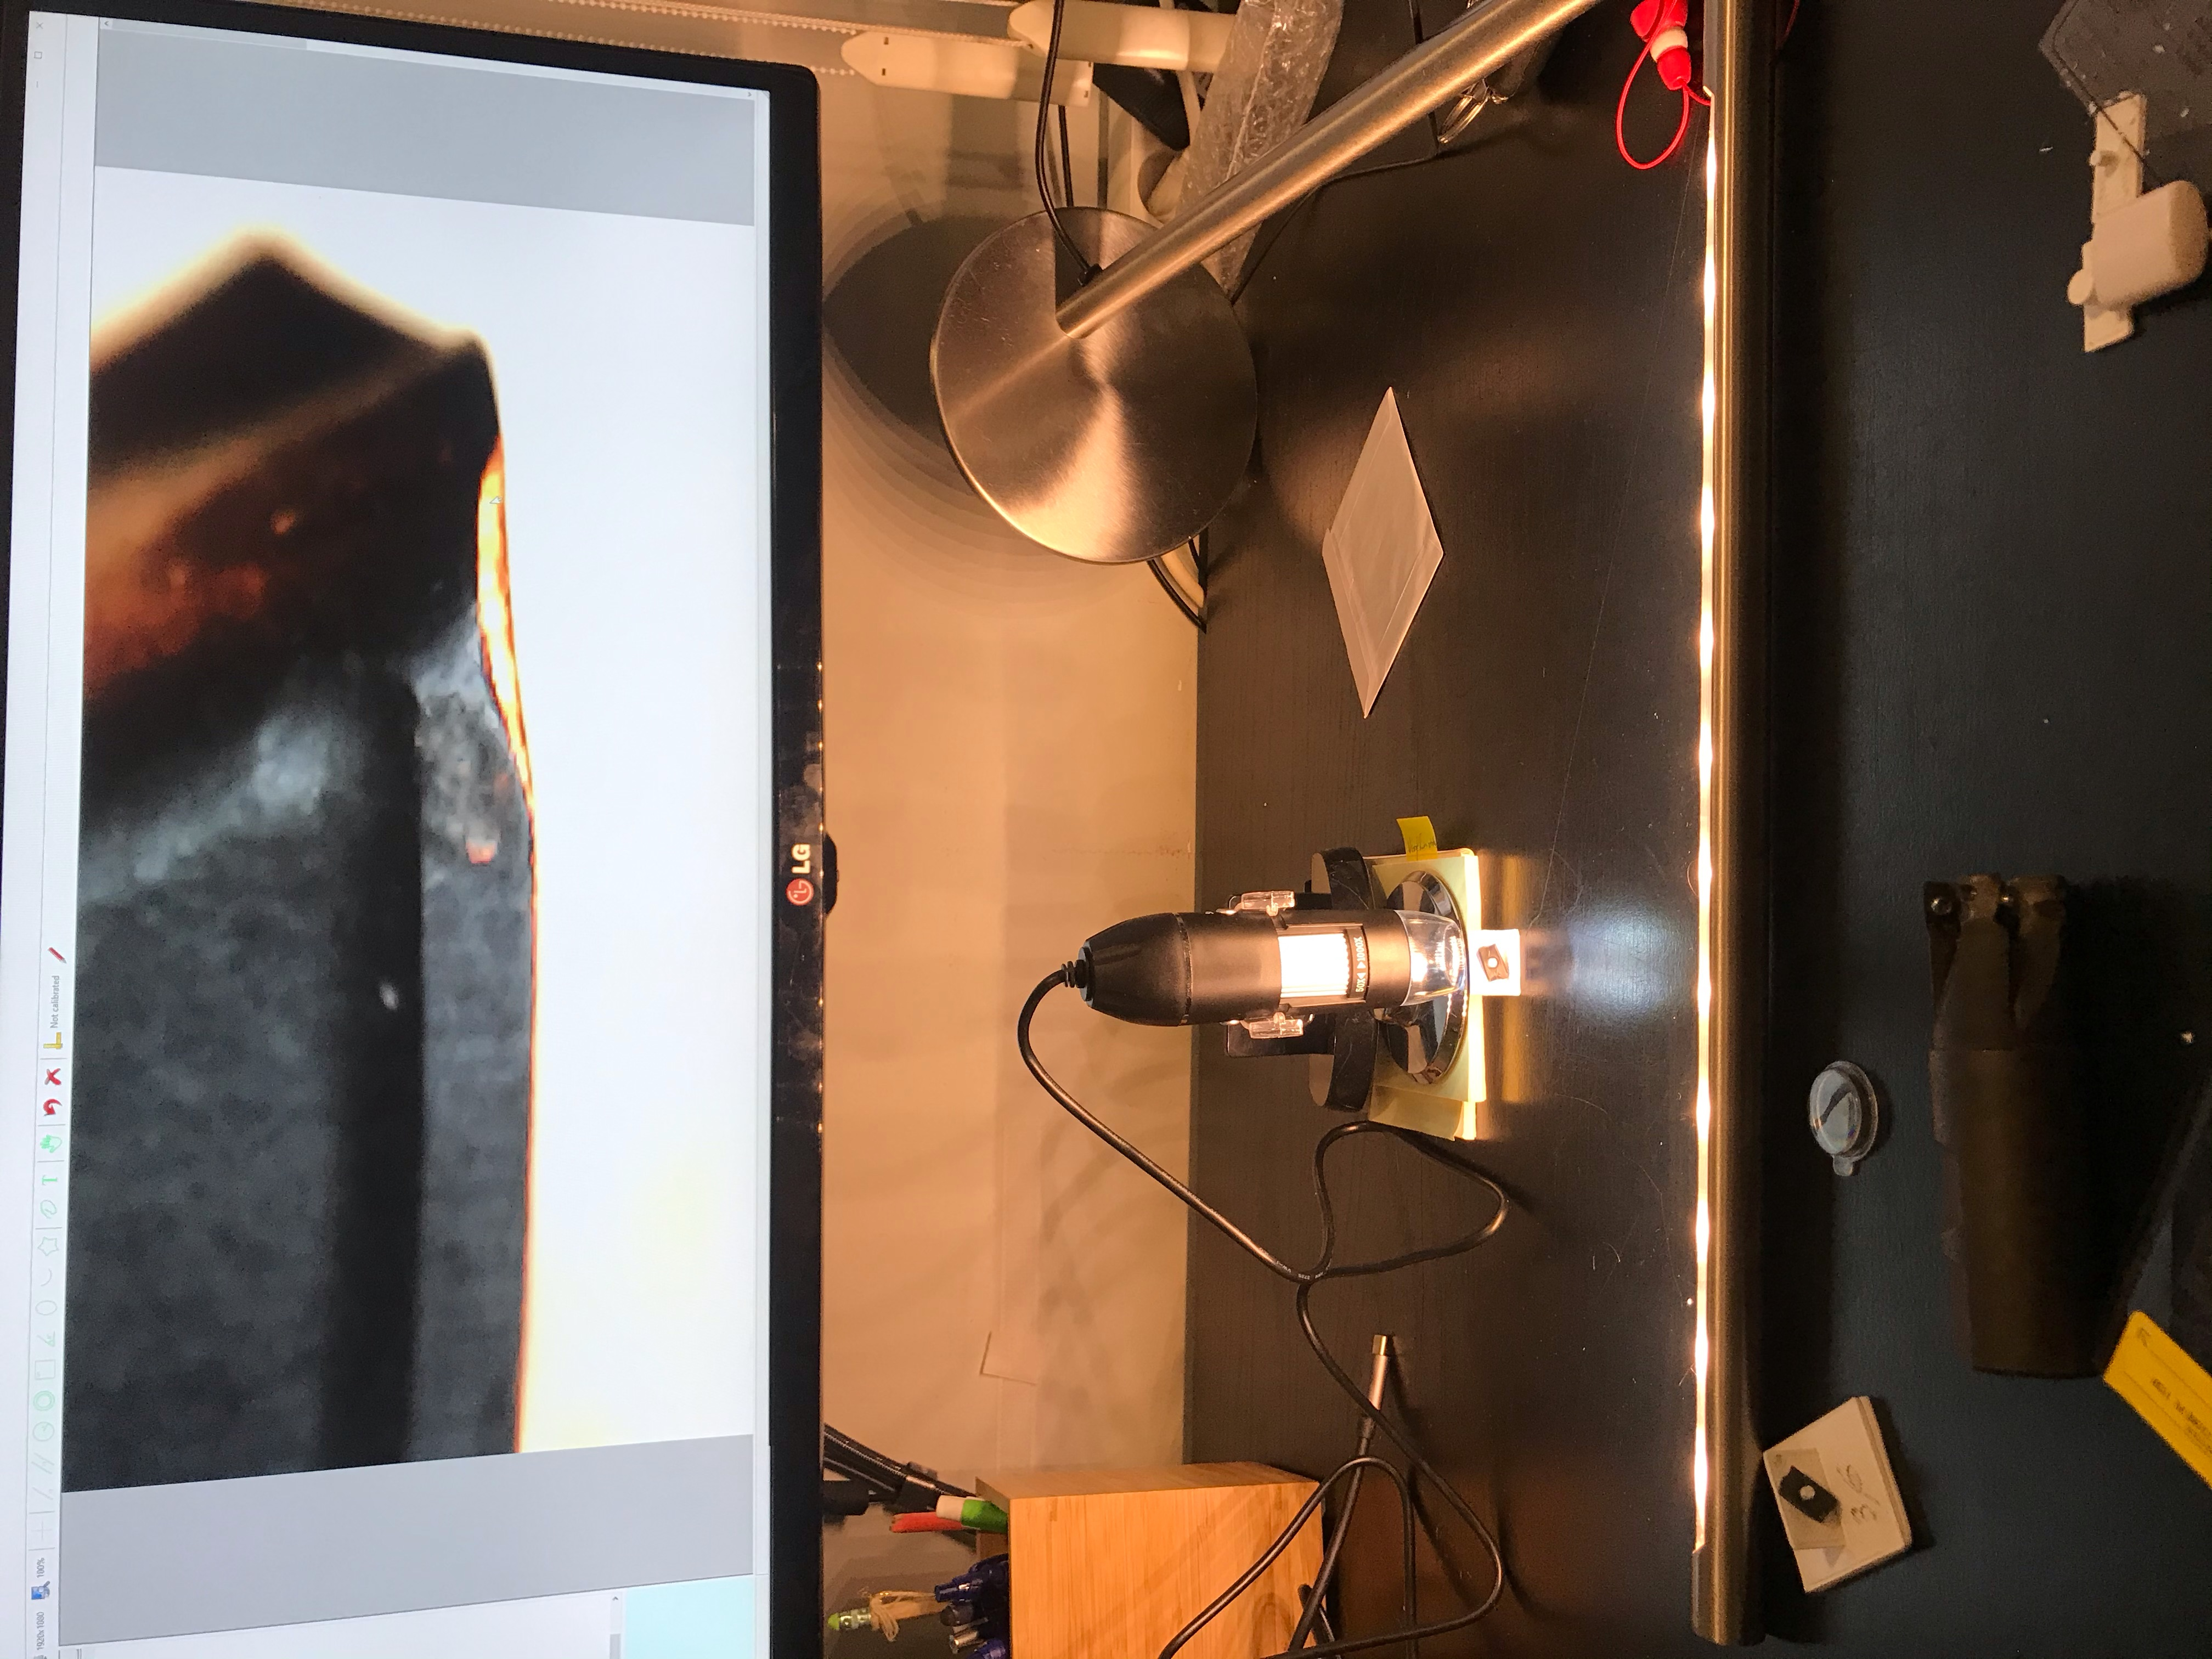
\includegraphics[width=4.166667in, keepaspectratio=true]{./ZimFiles_files/Camera_setup/Light/Desk_Lamp_Test/eerste_setup_andere_richting_beeld2.jpeg}



This setup was using the top light of the camera. This light was good to be able to adjust the camera. Without the light, the errornous places where more visible. But the desk lamp had to much brightness. Therefor and to test other lighting conditions a led strip will be used for further tests. 



The result with this setup can be seen in the above picture on the screen. here can be seen that there is a bright white background behind the tool. In a new setup there will be tried to make the background as dark as possible to make sure only the bad part of the tool is clearly lighted.



The result of this is shown in the following picture where the light is blocked off of the rest of the tool and only the errornous part is lightened. This would be a good start to start creating a dataset.



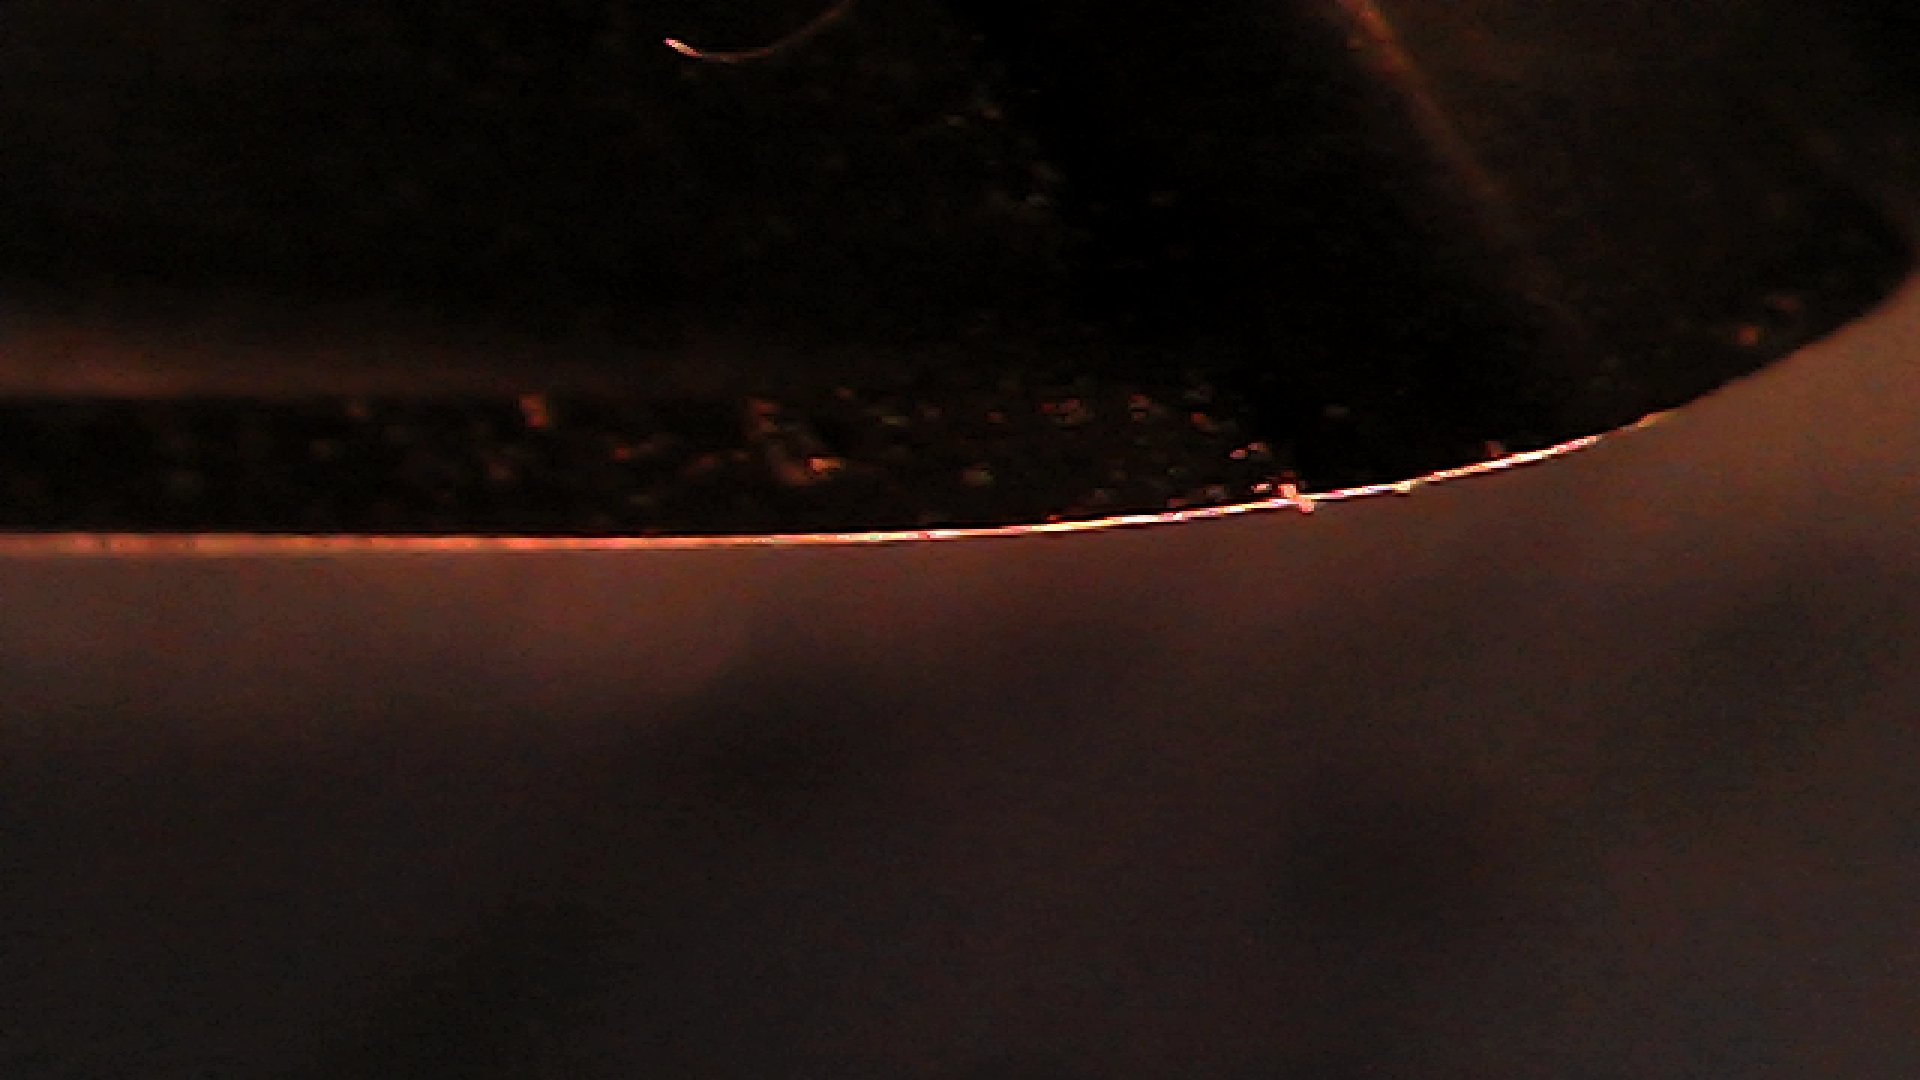
\includegraphics[width=4.166667in, keepaspectratio=true]{./ZimFiles_files/Camera_setup/Light/Desk_Lamp_Test/eerste-opstelling_donkere_achtergrond2.jpg}



The color of the desk light set a good gradient of bad vs good sets. White areas are worn very hard while orange is not worn that hard.



By tilting the lamp up and down in a horizontal way, all the areas where ligthtend. 



The setup used for this lighting scene is described 


		\section{White Led Strips}

Created Wednesday 28 October 2020



A second lighting contition created is the lighting with 3 the same led strips controllable with a raspberry pi. 

This was tested using some transistors to create a controllable switching circuit. This didn't work due to the wrong type of transistors. The second option is to control the led strips using proper relays. These will have to be bought separately so is must still be assessed if this is needed.



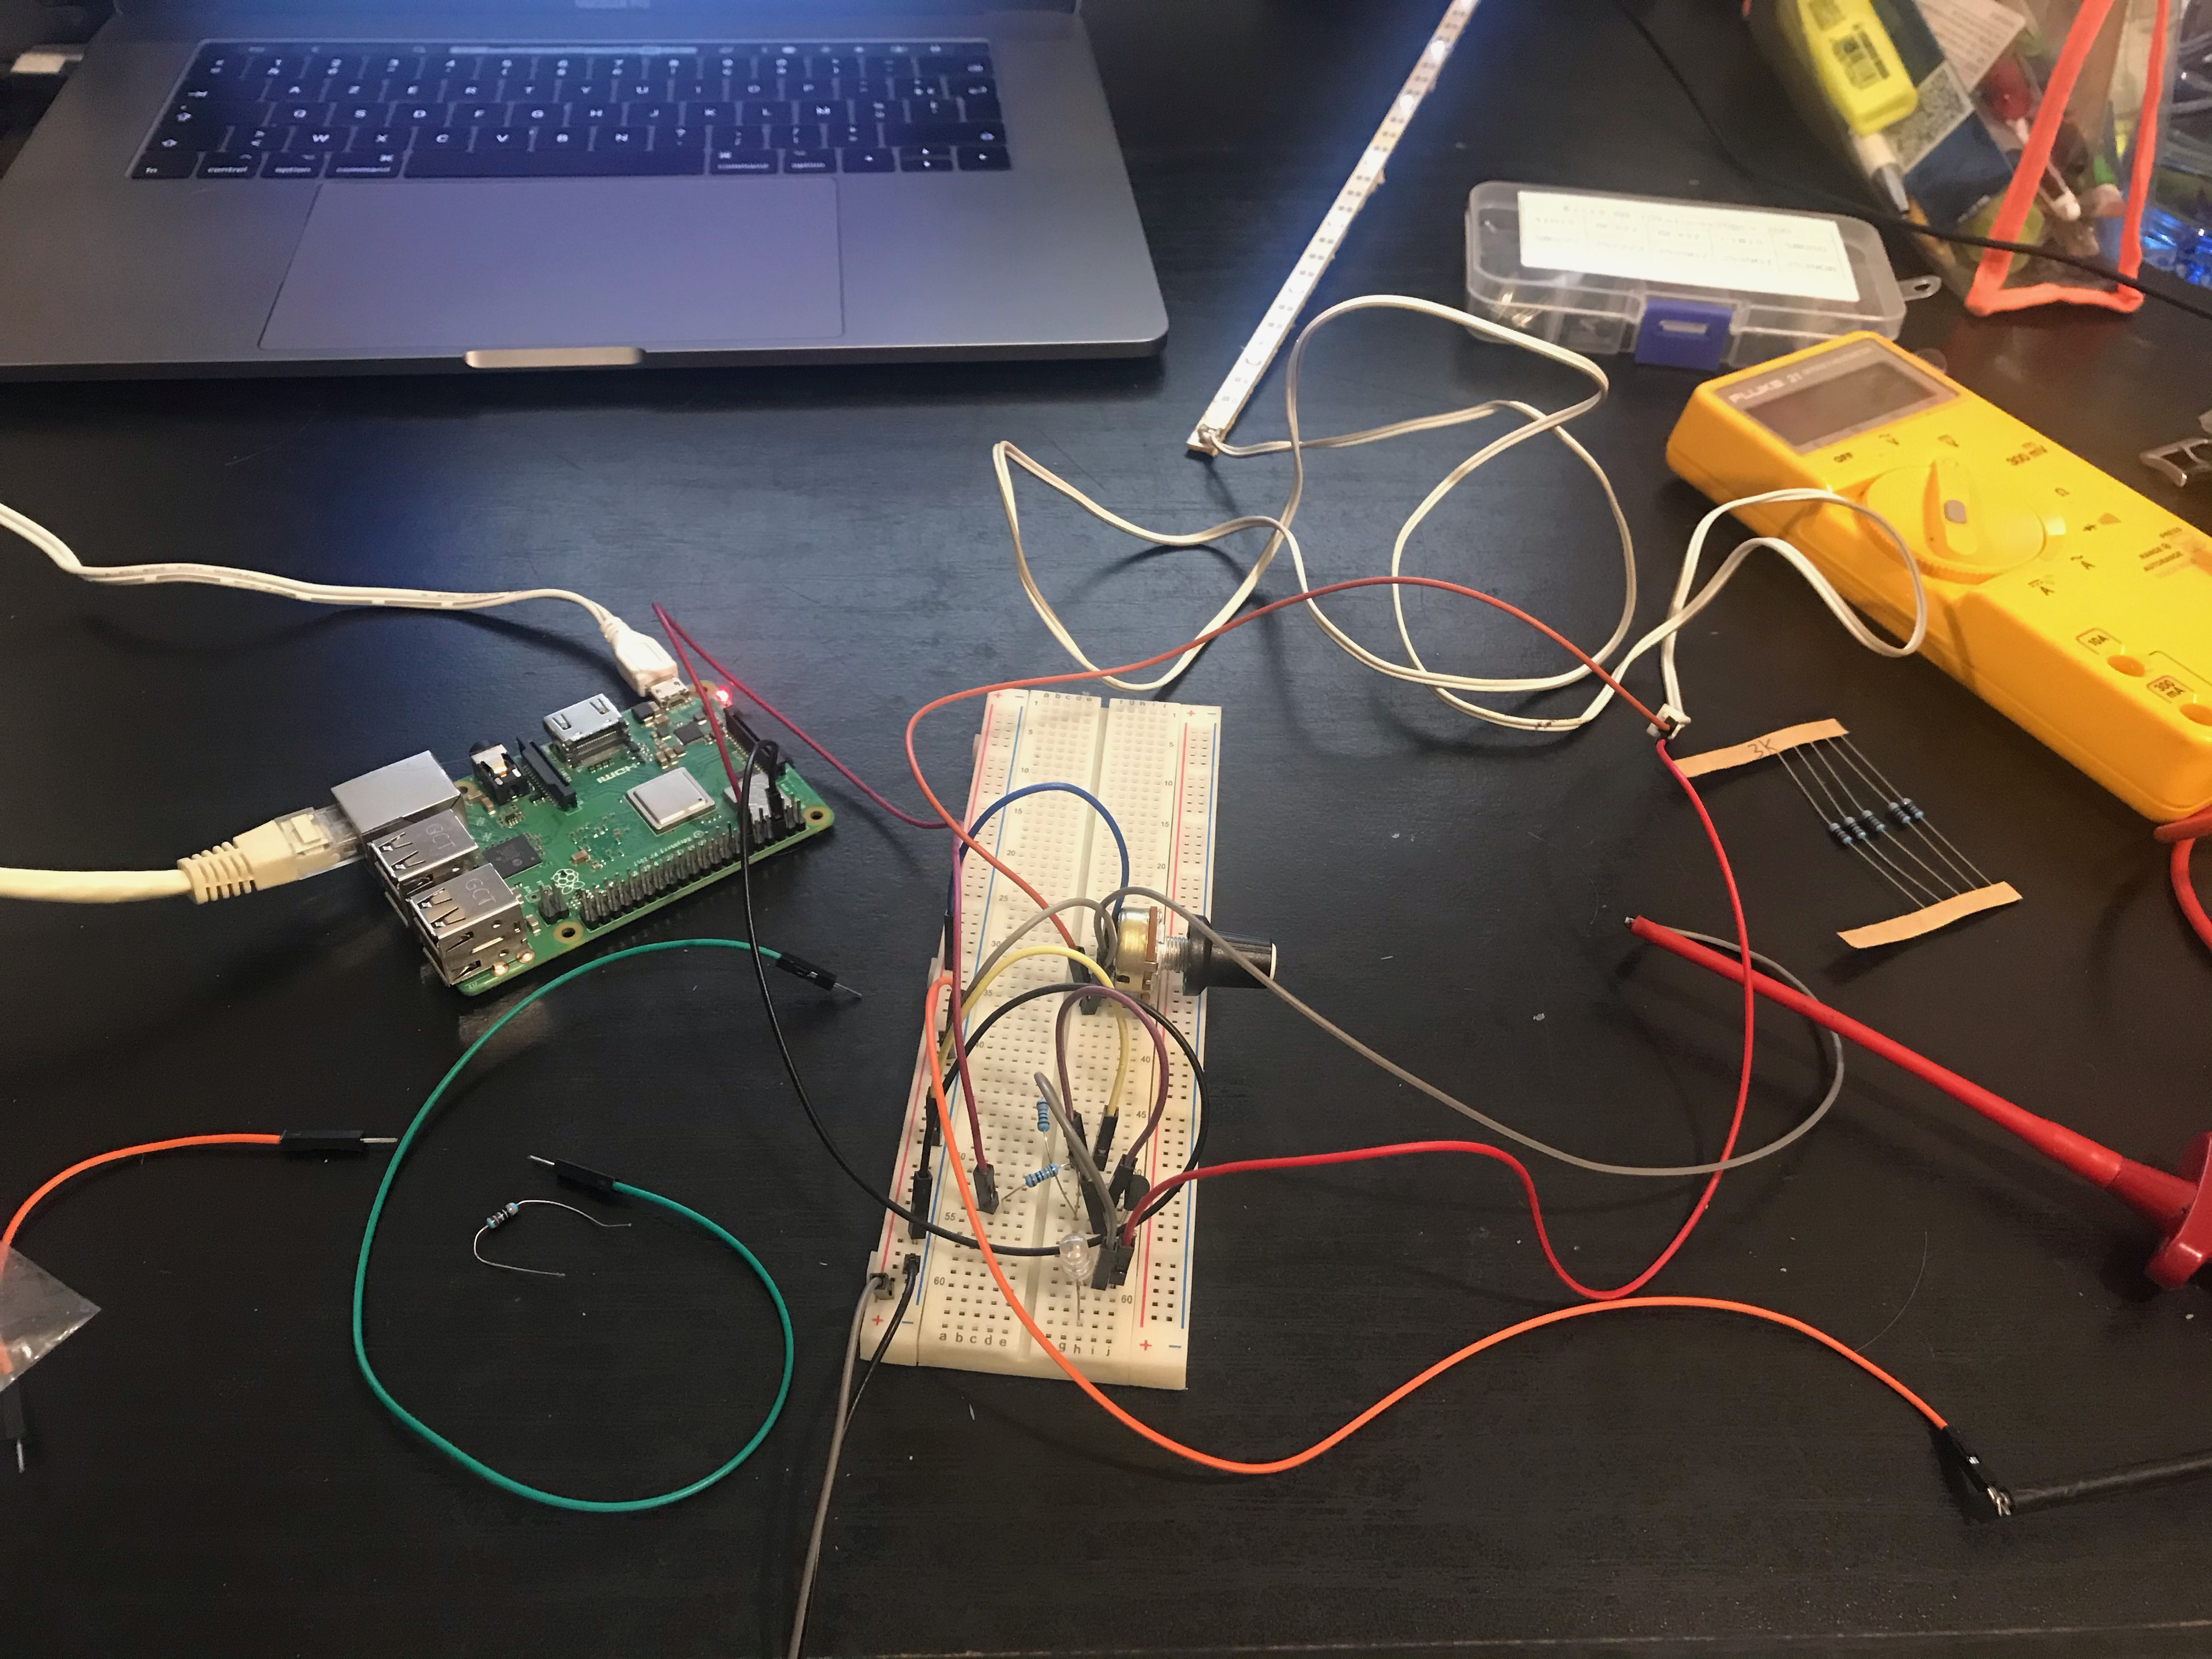
\includegraphics[height=3.125000in, keepaspectratio=true]{./ZimFiles_files/Camera_setup/Light/White_Led_Strips/Test_setup_ledstrip.jpeg}

The setup to test the control of a led strip using a NPN transistor as switch.


		\section{Tool Holder}

Created Wednesday 28 October 2020



During the design process different tool holders are designed to create an optimel camera position and optimal lighting conditions for that setup.




		\section{Simple holder}

Created Wednesday 28 October 2020



test remote second


		\section{Wheel Holder}

Created Wednesday 28 October 2020



\subsection{First Wheel Holder:}

A simple wheel holder which can hold 20 inserts.

used for first tests and did work. Except the tools wern't fixed good enough or they were to hard to remove and insert into the holder.

The holder was printed badly and this made the print cleanup very labor intensive. 



\subsection{Second Wheel Holder:}

Created on the base of the first wheel holder, but with an easier way of inserting and removing the tools. 

This with a more secure way of holding the tools. 

print so no cleanup must be done








		\section{first wheel holder}

Created vrijdag 13 november 2020



To be able to quickly create a lot of photos in a consistant way, a wheel is designed to mount 20 tools at once; using a stepper motor and a fixed camera and lighting setup the process of taking images would be automated for every 20 tools. The holder will be 3D printed so a few wheels can be made to be able to swap the wheels with new tools for an efficient dataset creation.



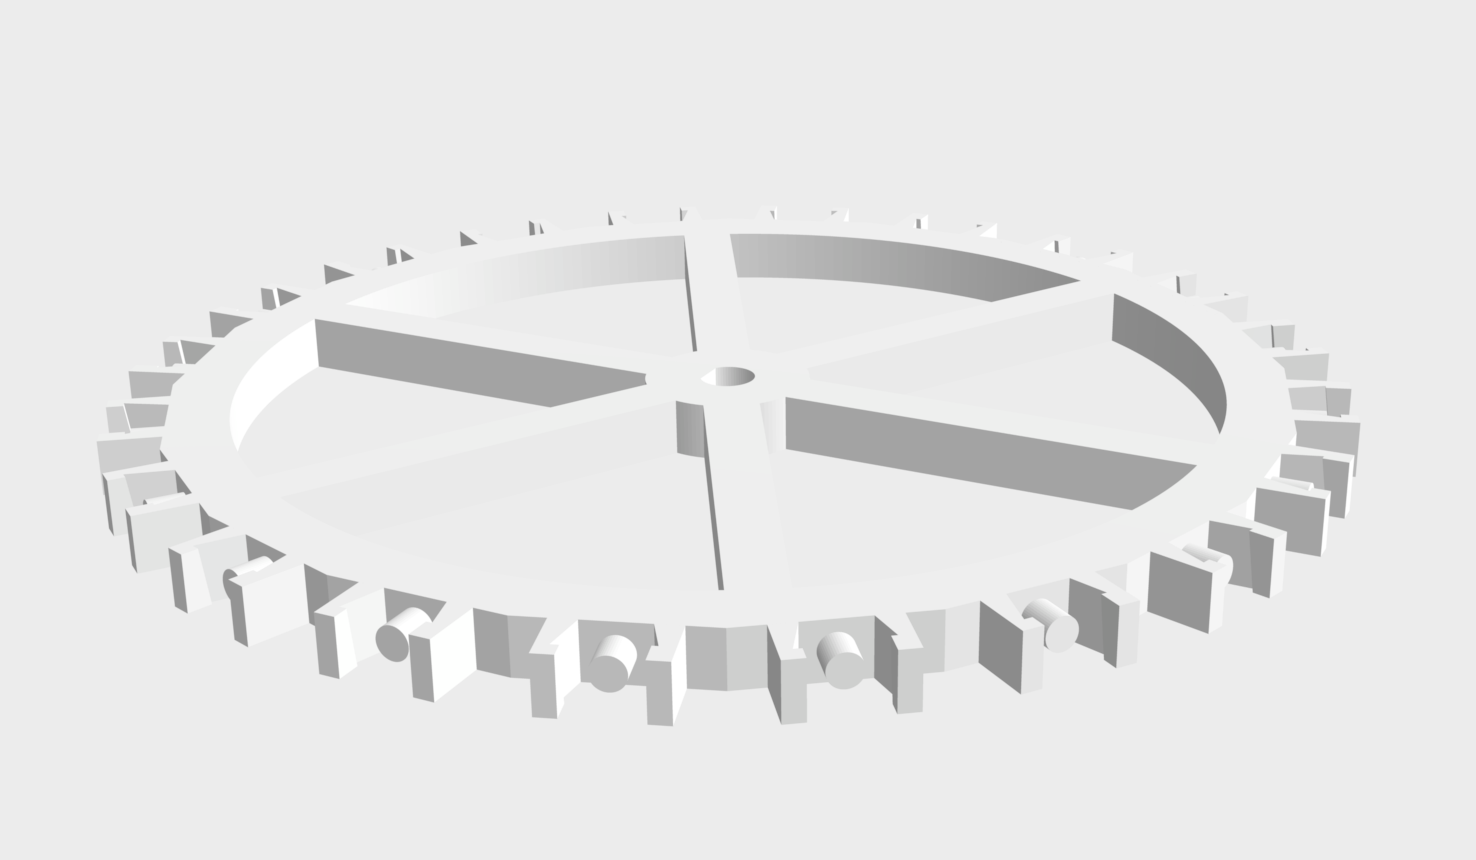
\includegraphics[height=3.125000in, keepaspectratio=true]{./ZimFiles_files/Camera_setup/Tool_Holder/Wheel_Holder/first_wheel_holder/radhouder.png}



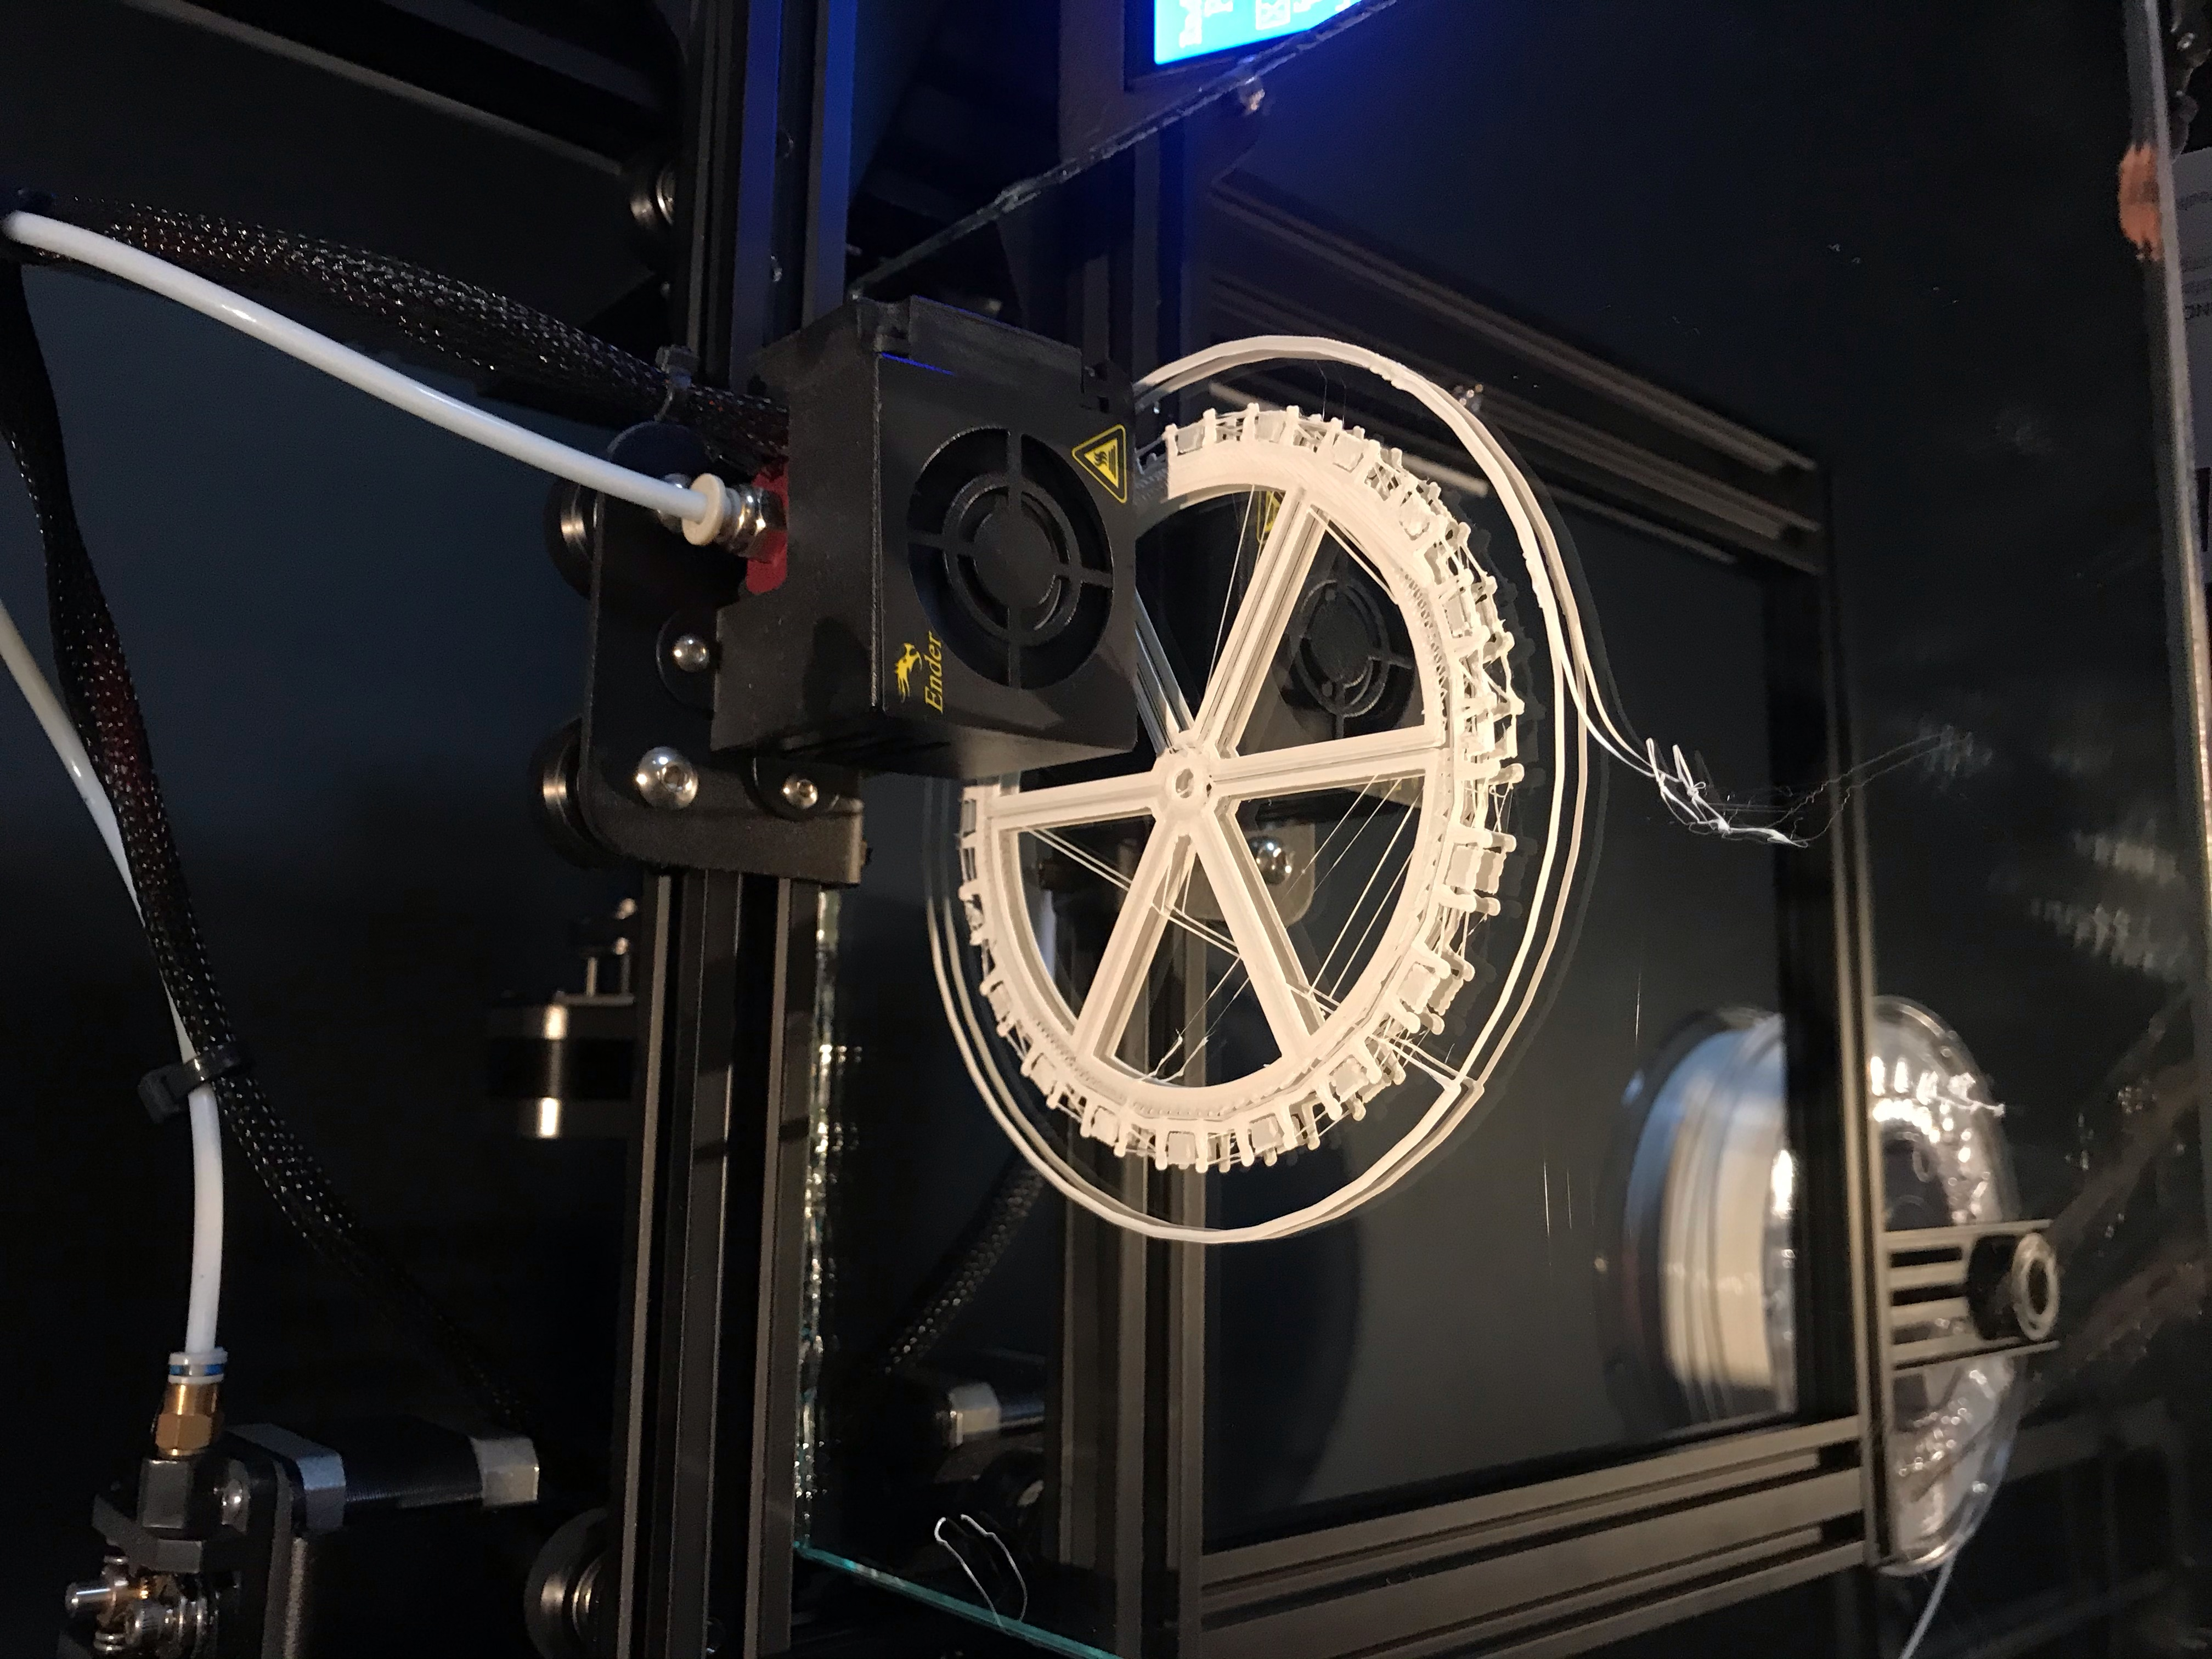
\includegraphics[height=3.125000in, keepaspectratio=true]{./ZimFiles_files/Camera_setup/Tool_Holder/Wheel_Holder/first_wheel_holder/radhouder_duringprint.jpeg}

After printing the wheel had to be cleared from rest pieces of plastic and had to be tested with a tool, this made it possible to scratch the tool extra hard which would mean the given labels for that tool aren't correct anymore. The tool used is from 3 number 6 36*. the manual removal also means the tools dont sit in the same position in every place on the wheel. This will show in the generated pictures.

\includegraphics[height=3.125000in, keepaspectratio=true]{./ZimFiles_files/Camera_setup/Tool_Holder/Wheel_Holder/first_wheel_holder/radhouder_horizontal.jpeg}



This wheel is mounted on a stepper motor with step angle of 1.8 degrees.

We can calculate the accuracy for a wheel with a radius of 5.5cm (measured to the tip of the measured tool) 

grad to radials

2*pi/360*1.8= 0.0314159265359

sin(0.031415)*55 = 1.72754081497 mm



this gives an accuracy of 1.72 mm, this is not in the accuracy range that is needed for this project. In order to get the wanted displacement per step the rotations needs to be adjusted with extra gears in the system. A displacement of less than 0.5 mm would be good.



to achieve this the calculations are made backworth:

the required angle

arcsin(0.5/55) = 0.52 degrees 

calculate how the gears should relate to each other

1.8/0.52 = 3.46153846154



round this up to 4 and recalculate the displacement per step of the motor

the angle:

1.8/4 = 0.45

2*pi/360*0.45= 0.00785398163397

sin(0.00785398163397)*55 = 0.431964548879mm



This is whithin the needed displacement range.



This needs adjustment of the current design of the wheel holder also a 3d printed footer can be printed so the wheel can circulate vertically which would make the camera and light setup easier.


		\section{Second Wheel Holder}

Created vrijdag 04 december 2020



The first wheel holder wasn't good because the inserts where clamped in with the knife side so it was very hard to remove them.

In a new wheel holder the clamps got changed by new clips that can easily be removed and printed again when the design changes. 

The inner tube that slides over the motor shaft is made bigger to fit over the motor axis.



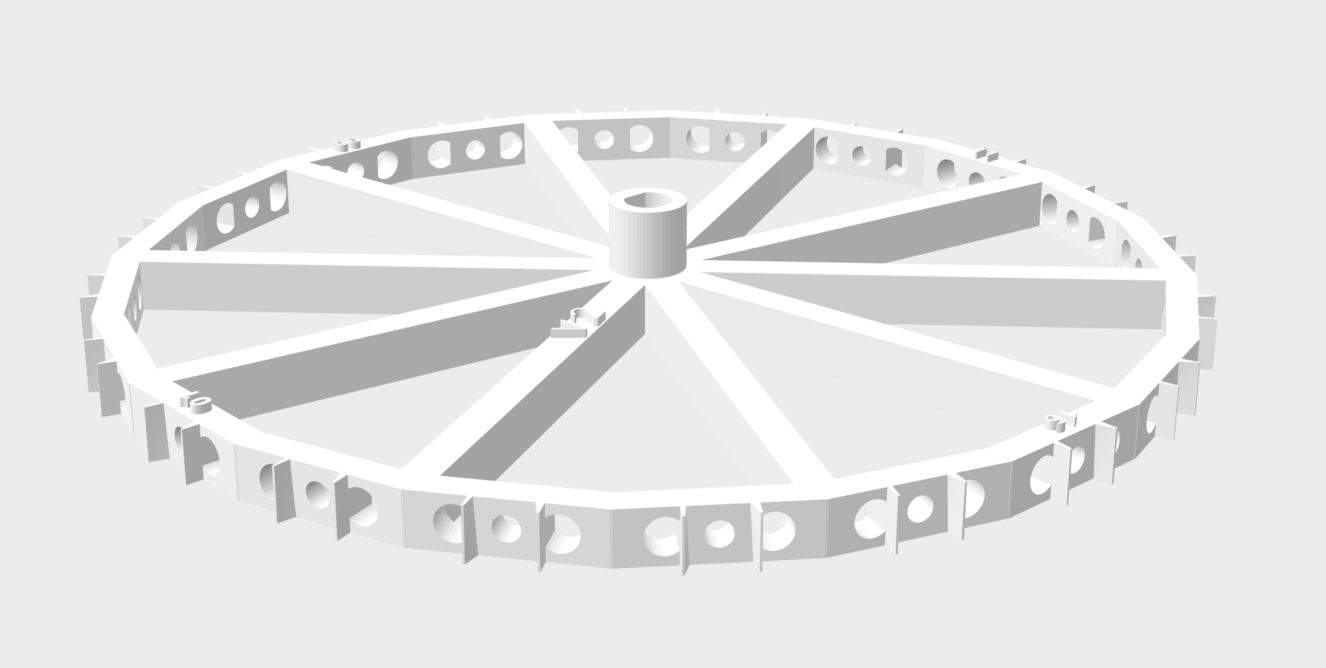
\includegraphics[width=5.208333in, keepaspectratio=true]{./ZimFiles_files/Camera_setup/Tool_Holder/Wheel_Holder/Second_Wheel_Holder/radhouder_v2.png}



In the wheel there are holes in which the clips fit. The center hole is as big as the hole in the inserts. This keeps the insert from moving round the hole.

The slads between the holes are made to fit the insert perfectly so this doesn't move or shift around. 



On the pictures the slads are visible which is not ideal so they will probably have to be adjusted in a future design.



The printing of these wheels was very difficult since it was with another material as we were used to and the print wouldn't stick to the print bed. This made a few bad runs and hours of wasted printing time. At the end 8 wheels of this are printed correctly and were used to create the Birthday dataset and the spaghetti dataset.



The clips looked like this:

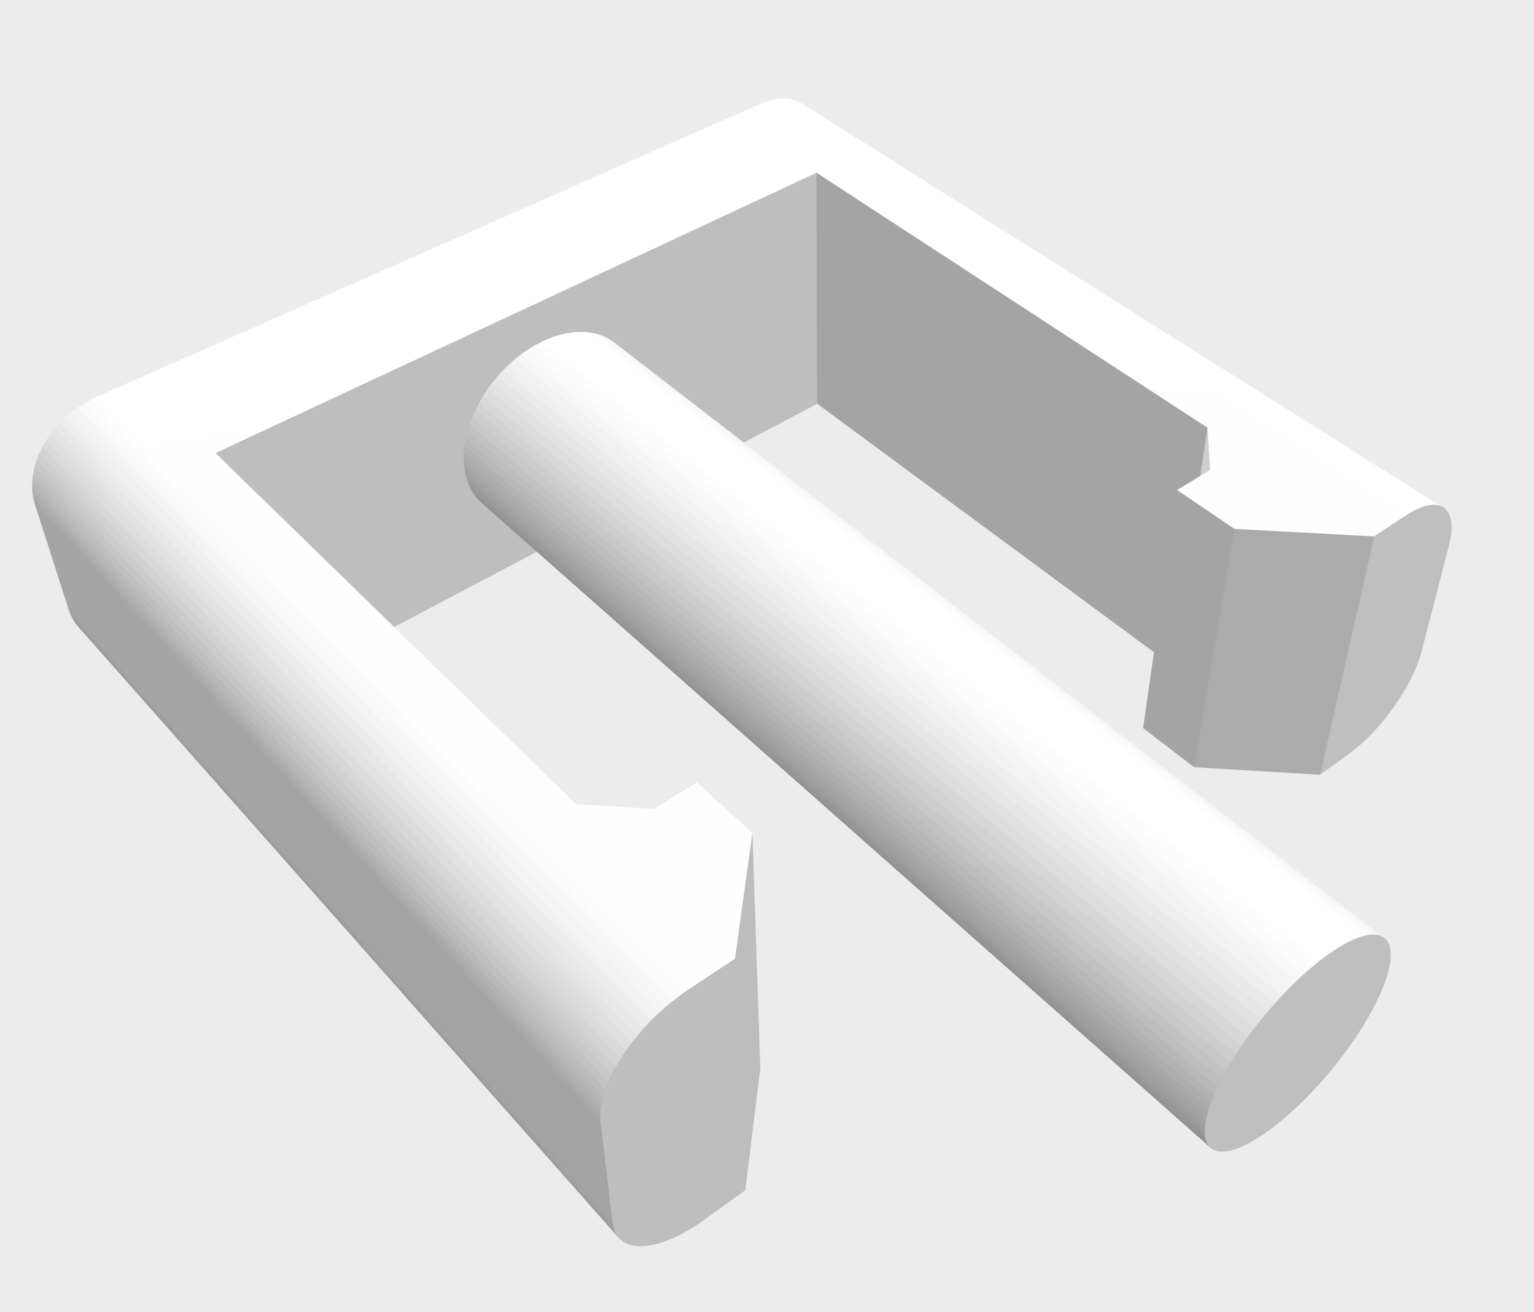
\includegraphics[width=3.125000in, keepaspectratio=true]{./ZimFiles_files/Camera_setup/Tool_Holder/Wheel_Holder/Second_Wheel_Holder/clip_9.png}


		\section{Code}

Created maandag 02 november 2020




		\section{Arduino}

Created maandag 02 november 2020



First project to control simple Led strips on off with mosfet and controll motor found on:

+motorLed






		\section{AdressableLed}

Created maandag 02 november 2020



Adressable led light controls



Led strip is a LPD8806


		\section{Control motor leds}

Created woensdag 02 december 2020



current working file is control\_motor\_leds






		\section{motorLed}

Created woensdag 11 november 2020



Here will the arduino code ./second\_test\_split\_strings.ino be discussed. Here are two addressable led strips, three long led strips and a stepper motor connected. 



the commands to be executed are the following

\begin{tabular}{ |l|l|l| }
\hline
 Commando & opties & output \tabularnewline
\hline
\hline
 LED STRIP &   &   \tabularnewline
\hline
 ------------ & -------- & -------------------------------------------------------------- \tabularnewline
\hline
 nrled & - & led off mode \tabularnewline
\hline
 nrled & + & led on mode \tabularnewline
\hline
 nrled & \_ & All leds off from set strip \tabularnewline
\hline
 nrled & xx & turn led with given index on or off depending on de set mode \tabularnewline
\hline
 nrled & +/-xx & change mode and turn led on/off \tabularnewline
\hline
   &   &   \tabularnewline
\hline
 brightness & -xx & lower brightness with xx amount \tabularnewline
\hline
 brightness & +xx & increment brightness with \tabularnewline
\hline
 brightness & \_ & set brightness to 0 \tabularnewline
\hline
 brightness & xx & set brightness to value xx \tabularnewline
\hline
   &   &   \tabularnewline
\hline
 startupleds &   & play green blue red on both ledstrips \tabularnewline
\hline
   &   &   \tabularnewline
\hline
 allon &   & turn all leds on white \tabularnewline
\hline
 alloff &   & turn all leds off \tabularnewline
\hline
   &   &   \tabularnewline
\hline
 ------------ & -------- & -------------------------------------------------------------- \tabularnewline
\hline
 Motor &   &   \tabularnewline
\hline
 ------------ & -------- & -------------------------------------------------------------- \tabularnewline
\hline
 step &   & repeat last settings for step \tabularnewline
\hline
 step & xx & repeat direction for xx steps \tabularnewline
\hline
 step & +/- & repeat number of steps in clockwise/counterclockwise direction \tabularnewline
\hline
 step & +/-xx & make xx steps in clockwise/counterclockwise direction \tabularnewline
\hline
 step & \_ & set number of steps to 0 \tabularnewline
\hline
   &   &   \tabularnewline
\hline
 q &   & turn everything off \tabularnewline
\hline
\end{tabular}

		
		
		\section{Problems}

Created vrijdag 13 november 2020



First problem encountered is that the communication or the delay between sending out a command from the python script and the action is pretty long -\textgreater{} 1.5s wait time before the next action can take place. this is to long..+arduino\_loop\_time searches the roots of this problem




		\section{arduino loop time}

Created vrijdag 13 november 2020



\subsection{Finding out the loop time}

To check where the delay is created, the time per arduino loop is printed out in micro seconds. Per function this time will be in the next table

\begin{tabular}{ |l|l|l| }
\hline
 Function & time in arduino & seconds in arduino \tabularnewline
\hline
\hline
 s & 999125 & 1 \tabularnewline
\hline
 nrled+160 & 1000922 & 1 \tabularnewline
\hline
 nrled+ & 1005941 & 1 \tabularnewline
\hline
 nrled & 1000597 & 1 \tabularnewline
\hline
 no command & 3 & 0 \tabularnewline
\hline
\end{tabular}




\subsubsection{First conclusions}

When too much is send before the loop ends; 

the delay becomes much bigger depending on the amount of data read. 

if we type nrleds 5 times with enters in between in a realy short time period -\textgreater{} less than 1s between the enters: the time of one loop will be 5 seconds.



\subsubsection{Finding out what takes so long in the loop}



\paragraph{Uncommenting all unnecessary FastLED.show functions}

with only one on the end of the function

creates following results:

\begin{tabular}{ |l|l|l| }
\hline
 Function & time in arduino & seconds in arduino \tabularnewline
\hline
\hline
 s & 1000669 & 1 \tabularnewline
\hline
 nrled+160 & 1000132 & 1 \tabularnewline
\hline
 nrled+ & 1000246 & 1 \tabularnewline
\hline
 nrled & 1000982 & 1 \tabularnewline
\hline
 no command & 3 & 0 \tabularnewline
\hline
\end{tabular}


This doesn't give better results



\paragraph{No FastLED.show functions}

\begin{tabular}{ |l|l|l| }
\hline
 Function & time in arduino & seconds in arduino \tabularnewline
\hline
\hline
 s & 999549 & 1 \tabularnewline
\hline
 nrled+160 & 1002195 & 1 \tabularnewline
\hline
 nrled+ & 1000931 & 1 \tabularnewline
\hline
 nrled & 1000211 & 1 \tabularnewline
\hline
 no command & 3 & 0 \tabularnewline
\hline
\end{tabular}


Conclusion;

The number of characters doesn't affect the time of the loop that much.



\paragraph{no ch = Serial.readStringUntil('$\backslash$n');}

if loop serial.available() is not entered the time elapsed is 3 microseconds.

when the loop is entered and nothing is passed in the string; an elapsed time of 850 microseconds is printed. 

when hardcoding nrled in the code instead of getting it from readStringUntil; the delay is around 950 microseconds. Not close to 1second



The problem must lay in the waiting for $\backslash$n;

possibly the algorithm waits for the $\backslash$n and if it doesn't come it will stop searching after a set delay



looking this function up in arduino reference manual gives the next output:

\uline{readStringUntil() reads characters from the serial buffer into a String. The function terminates if it times out (see setTimeout()).}



The setTimeout defaults to 1000 miliseconds. Whis is 1 second. if the input of the serial monitor is changed to the same but with $\backslash$n added to the end the next results pop up:

\begin{tabular}{ |l|l|l| }
\hline
 Function & time in arduino & seconds in arduino \tabularnewline
\hline
\hline
 s$\backslash$n & 1000313 & 1 \tabularnewline
\hline
 nrled+160$\backslash$n & 1000859 & 1 \tabularnewline
\hline
 nrled+$\backslash$n & 1000562 & 1 \tabularnewline
\hline
 nrled$\backslash$n & 1000367 & 1 \tabularnewline
\hline
 no command & 3 & 0 \tabularnewline
\hline
\end{tabular}




\paragraph{ch = Serial.readStringUntil('$\backslash$n') changed by  ch = Serial.readString();}

Serial.readString will also wait until the timeout is passed. 

Changing this timeout will repair the problem but this is dependant on the time it takes to read the bytes from the python script; this would be the same as from the arduino serial monitor normally.

Since the information is send at a rate of 9600 baud the time for one byte to be send is 1.04 miliseconds since one byte of send information contains a start and stop bit which results in 10 bits send.

With this information we can calculate how much miliseconds we need. Since the data that is send isnt more than 10 characters we can set the timeout at 10 miliseconds. This would speed things up by 100 times and would make the proces of taking pictures much smoother.



\begin{tabular}{ |l|l|l| }
\hline
 Function & time in arduino & seconds in arduino \tabularnewline
\hline
\hline
 s & 1001125 & 1 \tabularnewline
\hline
 nrled+160 & 1000968 & 1 \tabularnewline
\hline
 nrled+ & 1000636 & 1 \tabularnewline
\hline
 nrled & 1000884 & 1 \tabularnewline
\hline
 no command & 3 & 0 \tabularnewline
\hline
\end{tabular}




\paragraph{Serial.setTimeout(10)}

Set a timeout at 10 miliseconds at which the readString will stop reading. 

This should make the loop 100 times faster



\begin{tabular}{ |l|l|l| }
\hline
 Function & time in arduino & seconds in arduino \tabularnewline
\hline
\hline
 s & 10531 & 0.01 \tabularnewline
\hline
 nrled+160 & 11089 & 0.01 \tabularnewline
\hline
 nrled+ & 10236 & 0.01 \tabularnewline
\hline
 nrled & 10716 & 0.01 \tabularnewline
\hline
 no command & 3 & 0 \tabularnewline
\hline
\end{tabular}






This solution isn't ideal so a character must be send to conclude the sent string. Otherwise the rate of 10 miliseconds will always be lost. Trying a random character instead of $\backslash$n

ch = Serial.readStringUntil('/');  // $\backslash$n isn't detected



\begin{tabular}{ |l|l|l| }
\hline
 Function & time in arduino & seconds in arduino \tabularnewline
\hline
\hline
 s/ & 1192 & 0.001 \tabularnewline
\hline
 nrled+160/ & 1274 & 0.001 \tabularnewline
\hline
 nrled+/ & 1153 & 0.001 \tabularnewline
\hline
 nrled/ & 1132 & 0.001 \tabularnewline
\hline
 no command & 3 & 0 \tabularnewline
\hline
\end{tabular}




This solves the problem and times are 1000 times shorter than before. Now the tests from the python script can continue






















		\section{inception v3 won't run}

Created vrijdag 04 december 2020




		\section{Python}

Created woensdag 11 november 2020



+installation is done in the way described



A python script for test controlling the camera: +cameracontrol



Installation of pip +OpenCVinstallation



Required packages:+requiredPackages


		\section{cameracontrol}

Created woensdag 11 november 2020



Controlling the camera using



First test using following github page

https://gist.github.com/cbednarski/8450931 https://gist.github.com/cbednarski/8450931


		\section{installation}

Created woensdag 11 november 2020



\subsection{Install opencv}

\begin{enumerate}[1]
\item brew install python
\item pip install numpy
\item brew tap homebrew/science
\item brew install opencv
\end{enumerate}


\subsection{extra installation for pycharm}

\href{https://stackoverflow.com/questions/43372432/can-not-install-open-cv-on-my-pycharm-version-mac}{https://stackoverflow.com/questions/43372432/can-not-install-open-cv-on-my-pycharm-version-mac}

For installing OpenCV on Mac and using it in PyCharm, follow these steps:



Prerequisites: Python 2.7 or 3xx, virtualenv and OpenCV installed.



Open a terminal and create a virtual environment, pyimagesearch here



\$  mkvirtualenv pyimagesearch

Step 2 is miscellaneous, depending on your needs.



pip install numpy



pip install scipy



pip install matplotlib

Sym-link your cv2.so and cv.py files. (only cv2.so files for OpenCV 3xx ). On my system, OpenCV is installed in /usr/local/lib/python/2.7/site\_packages/



\$  cd ~/.virtualenvs/pyimagesearch/lib/python2.7/site-packages/



\$  ln -s /usr/local/lib/python2.7/site-packages/cv.py cv.py



\$  ln -s /usr/local/lib/python2.7/site-packages/cv2.so cv2.so

These steps are essentially for setting up this virtual environment for PyCharm.

Open up PyCharm and create a new "Pure Python" project



Set up the location of our Python Interpreter. By default, PyCharm will point to the system install of Python, however, for our case we need it to point to the virtual environment pyimagesearch.



So click on the gear icon and select "Add Local". In my case, the pyimagesearch  virtual environment is located in  ~/.virtualenvs/pyimagesearch/ with the actual Python binary in  ~/.virtualenvs/pyimagesearch/bin. Once you have successfully navigated to your folder, choose the virtual environment binary which is python2.7 in the bin folder for me.



Hope it helps!



After this, you are all set. PyCharm will use your pyimagesearch virtual environment and will recognize the OpenCV library.



\subsection{installation on virtual GNU}



\subsubsection{opencv install}

\href{https://docs.opencv.org/3.4/d7/d9f/tutorial_linux_install.html}{https://docs.opencv.org/3.4/d7/d9f/tutorial\_linux\_install.html}



packages installeren. 

\begin{enumerate}[1]
\item [compiler] sudo apt-get install build-essential
\item [required] sudo apt-get install cmake git libgtk2.0-dev pkg-config libavcodec-dev libavformat-dev libswscale-dev
\item [optional] sudo apt-get install python-dev python-numpy libtbb2 libtbb-dev libjpeg-dev libpng-dev libtiff-dev libjasper-dev libdc1394-22-dev
\end{enumerate}
directory aanmaken waar de source files in komen

/documents/opencv/opencv4.5


		\section{OpenCVinstallation}

Created woensdag 11 november 2020



\href{https://pypi.org/project/opencv-python/}{https://pypi.org/project/opencv-python/}



python3 -m pip install opencv-contrib-python



-\textgreater{} om python3 te kunnen gebruiken dat er voor zetten, ander wordt voor python 2 geinstalleerd


		\section{requiredPackages}

Created woensdag 11 november 2020



Packages installed using pycharm

\begin{tabular}{ |l|l| }
\hline
 Package name & used for \tabularnewline
\hline
\hline
 opencv & open camera \tabularnewline
\hline
 pyserial & control arduino \tabularnewline
\hline
\end{tabular}

		\section{Git}

Created vrijdag 13 november 2020



Git workflow:



Branches

\begin{itemize}
\item master
\item develop
\item feature/\textless{}feature-name\textgreater{}
\end{itemize}


Standard working;

\begin{enumerate}[1]
\item Git pull -\textgreater{} in correct map
\item work
\item git add \textless{}working folder name\textgreater{}/*
\end{enumerate}
4.git commit

	\begin{enumerate}[a]
	\item -m "commit text"
	\item -\textgreater{} just commit opens new editor window. first line short text than two empty lines and than long text for commit
	\end{enumerate}
\begin{enumerate}[1]
\setcounter{enumi}{4}
\item git pull
\item git push
\item git push origin \textless{}branch name\textgreater{} -\textgreater{} push to branch on remote git
\end{enumerate}


Creating new feature

\begin{enumerate}[1]
\item git checkout develop	-\textgreater{} go to develop branch
\item git branch -d feature/\textless{}feature name\textgreater{}		-\textgreater{} create branch
\item git push origin feature/\textless{}feature name\textgreater{}	-\textgreater{} push branch to remote
\item work
\item git checkout develop					-\textgreater{} set active branch to develop
\item git merge feature/\textless{}feature name\textgreater{}		-\textgreater{} merge branch to local current branch
\item edit files that couldn't be merged
\item git add \textless{}file name\textgreater{}
\end{enumerate}


Creating a tag 

\begin{enumerate}[1]
\item git tag 1.0.0 \textless{}first 10 characters of commit id\textgreater{}
\end{enumerate}

		\section{Research}

Created Wednesday 28 October 2020



\begin{enumerate}[1]
\item Study of the light reflection of the used tool material
\end{enumerate}




Type van eerste tools: 

\href{https://www.sandvik.coromant.com/en-gb/products/Pages/productdetails.aspx?c=R390-11%20T3%2008E-PL%20%20%201130&Country=be}{https://www.sandvik.coromant.com/en-gb/products/Pages/productdetails.aspx?c=R390-11\%20T3\%2008E-PL\%20\%20\%201130\$Country=be}




		\section{Light}

Created Wednesday 28 October 2020




		\section{Light Reflection}

Created Wednesday 28 October 2020



The next paper is good to get an overview of the light reflection seen in different types of materials and even multi layeres tools.

	article: \emph{New color from multilayer coating applied machining tools based on tungsten carbide insert}
	
	\begin{enumerate}[A]
	\setcounter{enumi}{9}
	\item \emph{C. Caicedo1}
	\end{enumerate}


Here is described that the best reflection occurs at the highest wavelength. This translates to the visible color red and will mean that the reflection should be the highest when the lighting is on the top of the spectrum of the camera lens. 



The material is best cut with a laser at wavelengths 1030nm and 515nm. This is proved in: 

	article: \emph{Fundamental investigations of ultrashort pulsed laser ablation on stainless steel and cemented tungsten carbide}
	
	is the good removal also a good reflector?
	
		

Study of absorption of certain wavelengths by the material. Not as usefull. unless all waves are absorbed by the material and only the rest is lightened. this is in the infrared spectrum so not realy possible with this camera.

	article: \emph{FTIR studies of tungsten carbide in bulk material and thin film samples}
	

		\section{tools}

Created woensdag 04 november 2020



Hoe slijt de tool? +Wear


		\section{Wear}

Created woensdag 04 november 2020



The wear of the tool begins with wear on the coating and goes right through the the coating in the base material of the tool. 

This base material will mostly be carbide due to its strength and heat resistance. 

	Slijtage is te zien in paper: Tool life and wear mechanism of uncoated and coated milling inserts
	
	Hier zijn alle slijtage types opgesomd
	
	

	The carbide used:
	
		cemented carbide here the combination with Wolfram called tungsten carbide
		
		in short WC Wolfram carbide
		
		

		more information on:
		
			\href{https://www.destinytool.com/carbide-substrate.html}{https://www.destinytool.com/carbide-substrate.html}
			
			



	






		\section{Vision Algorithm}

Created woensdag 18 november 2020



\subsection{Finding an algorithm to test the camera position setup}

First there must be found an algorithm that can quickly confirm wether a setup is good or not. This will be done by taking pictures different camera positions with the same lichting. After this the images go trough a simple model and the output is verified with a test set. 

This algorithm must be as small as possible to not have to take a lot of pictures to determine wether an algorithm is good or not. 






		\section{camera position validation}

Created woensdag 18 november 2020



\subsection{Information}

The next data input structure is made:

	\begin{itemize}
	\item 20 train images
	\item 10 validation images
	\item 10 test images
	\end{itemize}


These images will go through different algorithms multiple times and the outputs are verified for every different algorithm.



\subsection{papers}



\begin{enumerate}[1]
\item A Comprehensive Study on Deep Image Classification with Small Datasets
	\begin{enumerate}[a]
	\item short comparison of the amount of convolutional layers to be used in the network (5 is optimal)
	\item comparison on datasets: Caltech101, CIFAR10
	\item also transfer learning also around 5 convolutional layers is the optimum
	\item network architecture
		\begin{enumerate}[1]
		\item from scratch:
		\end{enumerate}
	\end{enumerate}
\end{enumerate}
			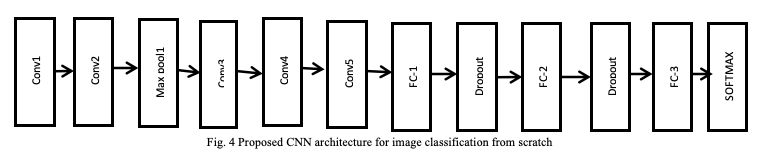
\includegraphics[]{./ZimFiles_files/Research/Vision_Algorithm/camera_position_validation/paper1_arch_fromscratch.png}
			
		\begin{enumerate}[1]
		\setcounter{enumi}{1}
		\item transfer learning pretrained on VGG16 with imagenet dataset
		\end{enumerate}
			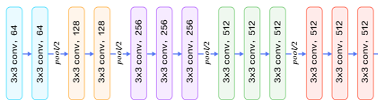
\includegraphics[]{./ZimFiles_files/Research/Vision_Algorithm/camera_position_validation/paper1_arch_transferlearning.png}
			
\begin{enumerate}[1]
\setcounter{enumi}{1}
\item Deep learning for image classifification on very small datasets using transfer learning
	\begin{enumerate}[a]
	\item creation of an image classification network with context of where it comes from
		\begin{enumerate}[1]
		\item alexnet vs googlenet vs vgg and the history
		\item displays keras code to create the same models
		\item architecture for models is shown
		\item niet super interessant gezien hier nog steeds wordt gewerkt op 6000 fotos van katten en honden, wel een indicatie dat deep learning gaat met weinig data
		\end{enumerate}
	\end{enumerate}
\end{enumerate}




\begin{enumerate}[1]
\setcounter{enumi}{2}
\item \href{https://paperswithcode.com/task/small-data}{https://paperswithcode.com/task/small-data}
	\begin{enumerate}[a]
	\item interesting papers with small datasets
	\end{enumerate}
\end{enumerate}


\begin{enumerate}[1]
\setcounter{enumi}{3}
\item A survey of the recent architectures of deep convolutional neural networks
	\begin{enumerate}[a]
	\item overview of almost all neural networks with their strengths and weaknesses
	\end{enumerate}
\end{enumerate}


\begin{enumerate}[1]
\setcounter{enumi}{4}
\item SDD-CNN: Small data-driven convolution neural networks for subtle roller defect inspection
	\begin{enumerate}[a]
	\item very interesting paper detects faults in bearing rollers. 
	\item Using very little data
	\item results with from scratch training best with SDD-inception v3 and SDD-resnet18
	\item SDD-VGG16 gets good results, but with long trainin time
	\end{enumerate}
\end{enumerate}


In most seen papers a very low learning rate 

0.0005 








		\section{Verslagen}

Created vrijdag 20 november 2020



\subsection{Inloopperiode verslag}

In te dienen op 7 oktober 2020

Ingediend op 7 oktober 2020



Hierin worden een aantal gegevens rond masterproef en -bedrijf vermeld:

\begin{itemize}
\item Voorlopige titel.
\item Informatie omtrent student(en): naam, adres, telefoonnumer, e-mail adres.
\item Informatie omtrent bedrijfspromotor(en): naam, bedrijf, adres, telefoonmummer, e-mail
\end{itemize}
adres.

De eigenlijke inhoud bevat minstens drie onderdelen:

\begin{enumerate}[1]
\item een beschrijving van de doelstellingen van de masterproef en de aflijning: welke elementen zullen onderzocht/uitgevoerd worden en welke niet;
\item een opsomming en korte beschrijving van de uitgevoerde activiteiten tijdens de inlooppe- riode, bijv. een theoretische studie, het opzoeken van relevante literatuur, ...;
\item een planning in de vorm van een Gantt kaart voor de volledige masterproef waarin een aantal deeltaken en mijlpalen opgesomd worden.
\end{enumerate}


\subsection{Activiteiten rapport 1}

In te dienen op 10 November



Tussen inloopperiode verslag en indienen van tussenstijds verslag

Deze rapporten bevatten een opsomming van 

\begin{itemize}
\item uitgevoerde activiteiten
\item opgetreden problemen en eventueel bijhorende oplossing
\item van uit te voeren activiteiten.
\end{itemize}
Zo’n rapport is incrementeel: het geeft de nieuwe elementen weer sinds de vorige rapportering.



\subsection{Tussentijds verslag}

In te dienen op 18 december 2020



tekst met probleemstelling, literatuurstudie en reeds gerealiseerde elementen

\begin{enumerate}[1]
\item Situering en doelstelling: een heldere, beknopte situering van de masterproef binnen een groter geheel op verschillende niveaus: wereld, Vlaanderen, het bedrijf of de onderzoeks- groep; en de beschrijving van de probleemstelling die aanleiding geeft tot de uitvoering van de masterproef; hieruit volgt dan een duidelijke omschrijving van de algemene en concrete doelstellingen van de eigen masterproef; voor een academisch georienteerde masterproef worden deze doelstellingen geformuleerd als onderzoeksvragen.
\item Literatuurstudie: weergave van de state of the art van het onderwerp: een korte beschrij- ving van de meest relevante (en actuele) referenties zodat de lezer een idee krijgt wat er op dit moment rond het onderwerp reeds beschikbaar is of onderzocht werd; bij elke geselec- teerde bron wordt een synthese gegeven van de relevante informatie; daarnaast kan ook de theoretische achtergrond van het onderwerp beschreven worden op basis van geraadpleegde literatuur.
\item Reeds gerealiseerde elementen: vaak is er reeds een eerste ontwerp of implementatie uit- gewerkt. Ook dit wordt in het tussentijds verslag opgenomen.
\item (Herwerkte) planning.
\end{enumerate}


De onderdelen probleemstelling en literatuurstudie van dit verslag moeten zodanig geschreven worden dat ze bijna integraal kunnen overgenomen worden als hoofdstukken 1 en 2 van de eindtekst.



Er is een \uline{checklist} beschikbaar (zie voorlaatste bladzijde) om de student te helpen alle nood- zakelijke elementen op te nemen in dit tussentijds verslag.



\subsection{Tussentijdse presentatie}

In te dienen op laatste examen dag



Elementen die bij deze presentatie aan bod komen zijn:

\begin{itemize}
\item Situering en doelstelling van de masterproef. Aangezien bij deze presentatie een aantal docenten aanwezig zijn, die niet rechtstreeks bij de masterproef betrokken zijn, moet de verwoording vrij helder en duidelijk zijn, zodat een leek in het vak zich een idee kan vormen over het onderwerp.
\item Reeds uitgevoerde taken: waarschijnlijk een analyse en een begin van ontwerp. Gemaakte keuzes moeten verantwoord worden, bijvoorbeeld met verwijzingen naar relevante literatuur en een evaluatie van de voor- en nadelen van de verschillende alternatieven.
\item Herwerkte planning, waarbij de actuele stand van zaken aangegeven wordt en de eventuele wijzigingen ten opzichte van de oorspronkelijke planning van in het begin van het
\end{itemize}
academiejaar.



Deze presentatie vindt plaats op de laatste examendag van de eerste examenperiode voor

een jury van OP1, OP2, OP3 en ZAP leden. Een precieze uurregeling wordt tijdig aan de studenten kenbaar gemaakt.

Voor één student wordt een tijdspanne van 15 minuten voorzien voor de presentatie, bij twee studenten mag dit oplopen tot 25 minuten:

\begin{itemize}
\item 40\%: situering problematiek - wat leidt tot de formulering van een onderzoeksvraag;
\item 50\%: voorgestelde aanpak voor de probleemoplossing met kritische reflecties (voorstudie/literatuurstudie, alternatieven/keuzes, mogelijke risico’s) en tussentijdse resultaten; 
\item 10\%: planning geven en motiveren.
\end{itemize}
Daarna is er en vijftiental minuten voorzien voor vragen van de juryleden en een mondelinge toelichting.

Na de bekendmaking van het behaalde resultaat (normaal in het begin van het 2e semester) geeft de promotor gedetailleerde terugkoppeling over het tussentijds verslag en de tussentijdse presentatie. Ook advies bij de verdere uitvoering van de masterproef mag van promotor verwacht worden.



\subsection{Activiteiten rapport 2}

In te dienen op 10 Maart



Tussen tussentijdse presentatie  en afwerking boek

Deze rapporten bevatten een opsomming van 

\begin{itemize}
\item uitgevoerde activiteiten
\item opgetreden problemen en eventueel bijhorende oplossing
\item van uit te voeren activiteiten.
\end{itemize}
Zo’n rapport is incrementeel: het geeft de nieuwe elementen weer sinds de vorige rapportering.


























		\section{Activiteiten rapport}

Created vrijdag 20 november 2020




		\section{Activiteiten rapport 1}

Created vrijdag 20 november 2020



Alle mails gelinkt hier



\subsection{Wat is er reeds gedaan deze periode tot 10 November?}



\subsection{Week 05/10/2020 - 11/10/2020}

opstellen en indienen van het tussentijds verslag in de eerste helft van de week.

Na 07/10/2020 was het verslag ingediend en werd gestart met het formuleren van een beschrijving van het probleem.

Het schrijven ging zeer moeizaam omdat ik weinig perspectief had over wat het doel van de masterproef was. Het is ook zeer moeilijk om een weg te banen tussen alle literatuur en de goede er tussenuit te vinden. Er werd heel wat tijd verspild met het lezen van bronnen die onvoldoende zijn of net niet goed genoeg waren. Hier moest een systeem in gevonden worden om de bronnen snel te kunnen inschatten. 



\begin{enumerate}[1]
\item bezoek gebracht aan Tom Jacobs van Sirris om de eerste plaatjes op te halen. 
	\begin{itemize}
	\item frees getoond en 
	\item uitleg gegeven over het bredere kader van het onderzoek. 
	\item Een verslag is hier te vinden. 
	\end{itemize}
\item Bedrijfs bezoek bij Aperam waar een vriend een visie inspectie systeem heeft geïnstalleerd dat fouten detecteerd in grote stalen platen. 
	\begin{itemize}
	\item Hier was het zeer nuttig om eens te zien hoe een systeem wordt geïmplementeerd in een productielijn. 
	\item De schaal was hier wel een stuk verschillend waardoor er niet echt dingen kunnen overgenomen worden.
	\end{itemize}
\item Start aan een beschrijving van het verleden van dit onderwerp.
	\begin{itemize}
	\item ging zeer moeizaam om dezelfde redenen als het zoeken van de probleem beschrijving.
	\end{itemize}
\item Implementatie maken voor een binair transfer learning model dat bepaald of een tool versleten is of niet. te vinden in \href{https://colab.research.google.com/drive/1N2r6nplmx88pUOKkLN0Hmy42D7YRUypC}{TWI 5} Dit bouwde verder op \href{https://colab.research.google.com/drive/1Qsoj7WmGClsslivGGI4DGL10NNVdIHC2}{TWI 4} waar een zelfde model werd gemaakt zonder tranfer learning.  \href{https://colab.research.google.com/drive/1Qsoj7WmGClsslivGGI4DGL10NNVdIHC2}{TWI 4} is een volledig werkend prototype van een algoritme in Keras.
\item implementatie maken voor een classificatie model \href{https://colab.research.google.com/drive/1QN68qaE84fq9dBnZFNExsS5F8tZk-8Ow}{TWI 6} in Keras waarbij tranfer learning wordt gebruikt. Hierbij waren alle voorspellingen voor dezelfde klasse. Niet verklaard hoe dit kon, misschien omdat de data niet gelijk verdeeld was over de klassen. De beste learning rates waren reeds bepaald voor dit probleem en lagen rond 3e-5 
\end{enumerate}


Voor alle bovenstaande tests werden de labels van labels3.csv gebruikt op de first handmade dataset





\subsection{Week 12/10/2020 - 18/10/2020}



\begin{enumerate}[1]
\item Verder schrijven aan het verleden van het onderwerp. 
	\begin{enumerate}[a]
	\item Ging zeer moeizaam en vergde veel tijd voor zeer weinig resultaat. 
	\item Gekomen tot een aantal bronnen. 
	\item opzetten mendeley om bronnen in bij te kunnen houden.
	\end{enumerate}
\item Aanmaken van Engelse latex file op overleaf
\item implementatie maken in keras waarbij een regressie model wordt getraind op de eerste honderd foto's die verkregen zijn
	\begin{enumerate}[a]
	\item fotos te vinden als first handmade dataset
	\item Een regressie model wordt niet ondersteund door Keras waardoor het zeer omslachtig was om de labels en de foto's met elkaar te kunnen verbinden. Dit zorgde voor heel wat problemen.
		\begin{enumerate}[1]
		\item classificatie model met transfer learning maken met Keras dat de gegevens opdeeld in 3 klassen waarbij ook een verschillende batch size werd getest. Te zien in \href{https://colab.research.google.com/drive/1QN68qaE84fq9dBnZFNExsS5F8tZk-8Ow}{TWI 6} en  \href{https://colab.research.google.com/drive/1zeKin3shLk_ogrFCwHrzpnjJmaWaoCq0#scrollTo=CDnGBD0NGkbM}{TWI 7}
		\item proberen de labels toch gelinkt te krijgen via de data loader functies van Keras. Dit werkte echter niet dus werd een andere methode geprobeerd
		\item Het regressie probleem omzetten in een classificatie model wat betreft de data. Hiervoor werd een map aangemaakt per waarde en dus per foto om zo de gegevens in te lezen. Dan werd de model architectuur aangepast zodat deze een output gaf van een getal waarde in dezelfde grootte orde als de waarden van de metingen. 
		\end{enumerate}
	\end{enumerate}
\end{enumerate}
			Dit werkte echter ook niet en er werden geen resultaten bekomen.
			
			De uitwerking is te vinden op Google Colab onder de naam \href{https://colab.research.google.com/drive/1qR4reWAIvIs59eZKWSmZHboZ1gjGA4jS}{TWI 8} waarbij ook transfer learning werd toegepast om de weinige data toch te kunnen omzetten in een werkend model
			
\begin{enumerate}[1]
\setcounter{enumi}{3}
\item Er werd gekeken welke andere frameworks er nog zijn en wat het verschil is tussen deze. Hier is ook beslist om verder te gaan met Pytorch gezien dit het meest open framework is. 
\end{enumerate}


\subsection{Week 19/10/2020 - 25/10/2020}



\begin{enumerate}[1]
\item Een nieuwe implementatie \href{https://colab.research.google.com/drive/1f-Rfei8QrHotvgktp8hzviR8dv1XJJjz}{TWI 9} waarin een eerste model werd gemaakt met pytorch. 
	\begin{enumerate}[a]
	\item er werden wat problemen gevonden bij het tonen van de foto's eens ze genormaliseerd waren waardoor het moeilijk was om de data voor te stellen die gebruikt werd. 
	\item Een model van het internet werd geïmplementeerd en er werden resultaten bekomen ± 60\% accuracy op de train en validation data. Dat lijkt niet zo correct. op een test set van slechts enkele beelden werd 25\% accuracy gehaald. Er leek ergens iets mis te zijn met de transformaties van de foto's naar pil voorstelling. 
	\end{enumerate}
\item Een binaire classificatie implementatie \href{https://colab.research.google.com/drive/1t4Yvzj1rqNy24pj4dDtyBH2CStDePXMw}{TWI 10} werd gemaakt waarin een zelfde model architectuur werd geprobeerd te maken als bij het model van Keras. 
	\begin{enumerate}[a]
	\item Echter was dit zeer lastig zonder voorkennis van hoe architecturen er uit zien. Door het sterk verschil in benamingen tussen functies is dit niet geslaagd. 
	\item De foto's in juiste mappen plaatsen via een programma werd ook gerealiseerd na heel wat problemen met de google colab mappen structuur. 
	\item In het model waren de data augmentation regels te hard. Hierdoor werden de foto's zeer sterk bewerkt wat zorgde voor heel wat meer foto's, maar tegelijk deed het afbreuk aan het model gezien de foto's in het echt makkelijker te interpreteren vallen. 
	\item De training en validation loss ging niet naar beneden tijdens de training.
	\end{enumerate}
\item Meeting met Dries Hulens waarin werd overlopen hoe de opstelling zou gemaakt worden en waar op te letten.
	\begin{enumerate}[a]
	\item hierbij werd aangehaald dat het schrijven nog niet belangrijk zou zijn, en dat dit nog even kon wachten tot december eventueel.
	\item licht reflecties onderzoeken hoe het materiaal reageerd op bepaalde licht frequenties.
	\item eventueel kijken of een stuk uit de fotos kan gesneden worden (felste blob) om enkel daar het model mee te voeden.
	\item adresseerbare ledstrip mee gekregen
	\item camera mee gekregen.
	\end{enumerate}
\item Een eerste testopstelling maken om de camera te leren gebruiken.
	\begin{enumerate}[a]
	\item De camera moest zeer goed ingesteld worden om een scherp beeld te krijgen van de slijtage
	\item Setup is besproken in: first camera mount
		\begin{enumerate}[1]
		\item hiervoor is een houder ge 3D print.
		\item De belichting besproken in desk lamp test
		\item de camera werd met denormale houder op de bureau gezet. 
		\end{enumerate}
	\item De beelden hiervan waren zeer indrukwekkend en gaven een mooi resultaat zonder veel werk te hoeven steken in een setup.
	\end{enumerate}
\end{enumerate}


\subsection{Week 26/10/2020 - 1/11/2020}



\begin{enumerate}[1]
\item 3D model gemaakt van het eerste rad dat gebruikt zal worden voor een automatisch systeem dat de plaatjes voor de camera beweegt.
	\begin{enumerate}[a]
	\item Creatie van een 3D model
	\item 3D printen 
	\item berekening welke nauwkeurigheid nodig is om de stappen motor aan te sturen
	\end{enumerate}
\item Een programma aangemaakt om de stepper motor aan te sturen met de motor drivers. 
\item documenteren van de afgelopen tests
\item Test met vaste led strips om ze te kunnen aansturen vanaf een raspberry pi
	\begin{enumerate}[a]
	\item Ging niet goed met zeer kleine transistors. 
	\item overgeschakeld naar relais. Gaf zeer veel problemen met solid state relais die ook in gesloten toestand nog een stroom doorlieten.
	\item Gewone analoge stuurbare relais werkten wel, maar maken een klik geluid. 
	\item Volgende stap is om mosfets te gebruiken voor deze sturing.
	\item Test met verschillende voltages met een potentiometer voor de strips.
	\end{enumerate}
\item PCB maken om de aansturing mogelijk te maken gezien het breadboard de hoge stroom niet aan kan. 
\end{enumerate}


\subsection{Week 02/11/2020 - 08/11/2020}



\begin{enumerate}[1]
\item Ophalen van een volgende batch plaatjes
	\begin{enumerate}[a]
	\item bekijken hoe de plaatjes worden gelabeld. 
	\item opzoeken en documenteren of de plaatjes reageren op een bepaalde golflengte zonder goede resultaten, dit moet nog verder onderzocht worden.
	\item materialen van de plaatjes opzoeken
	\item Afslijting komt recht op de hoek van het plaatje
	\item Frees kan niet zelf nauwkeurig draaien, een mogelijke oplossing is de voledige snijplaat houder uit de frees halen en fotograferen.
	\item Er zijn ongeveer 4 hoofdklassen van slijtages, maar deze zijn moeilijk zelf na te maken
	\item Een extra metric toevoegen die de oppervlakte van de slijtage weergeeft. 
	\end{enumerate}
\item Een testopstelling gemaakt met het rad met de stepper motor en enkele bandijzers om de leds aan te bevestigen.
\item Arduino finetunen zodat deze volledig werkt met de adressable led en de motor makkelijk kan aangestuurd worden met commandos via de seriele input.
\item Eerste beelden maken met een geautomatiseerde setup
	\begin{enumerate}[a]
	\item zie first automated dataset
	\item werkte niet, de communicatie tussen de computer en arduino was te traag. Dit wordt (tijdelijk) opgelost door delays te plaatsen die de trage communicatie opvangen. 
	\item Eerste beelden konden gemaakt worden en het python script is gemaakt.
	\end{enumerate}
\item PCB finetunen 
	\begin{enumerate}[a]
	\item nieuwe weerstand die de spanning begrensd voor de ledstrip
		\begin{enumerate}[1]
		\item is doorgebrand en terug vervangen door een grotere weerstand
		\end{enumerate}
	\end{enumerate}
\end{enumerate}




\subsection{Wat er nog zal gebeuren voor de tussentijdse presentatie}

\begin{enumerate}[1]
\item Afwerken van de setup en oplossen 
\end{enumerate}





		\section{Activities}

Created vrijdag 20 november 2020



Update mails en meetings sinds 6 oktober ( na inloopperiode verslag) zijn hieronder gelinkt. 

Ze worden besproken in activiteiten rapport 1



\begin{enumerate}[1]
\item 09/10/2020: Masterproef Tool Wear Inspection - Meeting1 TJ
\item 14/10/2020: Masterproef Tool Wear Inspection - Update 1 DH
\item 21/10/2020: Masterproef Tool Wear Inspection - Meeting2 DH
\item 29/10/2020: Masterproef Tool Wear Inspection - Update 2 DH
\item 29/10/2020: Masterproef Tool Wear Inspection - Update 3 TJ
\item 04/11/2020: Masterproef Tool Wear Inspection - Meeting3 TJ
\item 12/11/2020:Masterproef Tool Wear Inspection - Update 3 DH
\end{enumerate}


		\section{Masterproef Tool Wear Inspection - Meeting1 TJ}

Created vrijdag 20 november 2020



Notities van de meeting

./meeting 20201009.pdf



Korte samenvatting:

\begin{itemize}
\item Tegen eind oktober 200 extra plaatjes
\item Na nieuwjaar kijken hoeveel “echte” plaatjes nodig zijn om de soorten slijtage op te kunnen bepalen
\item Nauwkeurigheid die gehaald zou moeten worden is 20 micrometer
\item Plaatje is slecht vanaf het een slijtage heeft van meer dan 200 micrometer (best iets vroeger kunnen zeggen dat het plaatje de grens van 200 micron zal overschrijden)
\item Hoe de inspectie nu gebeurt:
	\begin{itemize}
	\item Uithalen en bekijken met blote oog of lens
	\item Elke vaste tijdspan verwisselen
	\end{itemize}
\item Maandelijkse update om vooruitgang te bespreken
\item Verschillende coatings moeten ook onderzocht worden
\item Kostprijs mee bekeken voor de hele setup
\end{itemize}

		\section{Masterproef Tool Wear Inspection - Meeting2 DH}

Created vrijdag 20 november 2020



Meeting 21/10/2020

Dries Hulens



Plaatjes tonen



Camera opstelling maken 

-	Licht? -\textgreater{} led

o	\href{https://www.ni.com/en-gb/innovations/white-papers/12/a-practical-guide-to-machine-vision-lighting.html}{https://www.ni.com/en-gb/innovations/white-papers/12/a-practical-guide-to-machine-vision-lighting.html}

Eender wat checken golflengte 

Zien bij welke frequentie het materiaal waarmee het plaatje gemaakt is het meeste licht weerkaatst.  Zo sneller nuttig van onnutig scheiden op de beelden



-	Camera setup tools

Statief/ houder -\textgreater{} twee kanten tegelijk nakijken

 3d printen om de opstelling te maken 



-	Lenzen

20px per fout -\textgreater{} 20micron fout meten -\textgreater{} 1px per micron detecteren

	Resulutie is hoog genoeg om de fouten te detecteren, eventueel kan een hogere resolutie gewenst zijn als de soorten fouten moeilijk zichtbaar zijn



Schrijven workflow?

	Lezen en meteen wat typen over het artikel?
	
		Goed -\textgreater{} nog niet te veel schrijven, eerst veel testen
		
Schrijven kan op 2 weken als alles goed gedocumenteerd is tijdens de testen

	Hoeveel moet gefundeerd worden met artikels? -\textgreater{}meer tijd steken in testings?
	
	Artikels voor alles wat opgezocht moet worden, de rest gewoon testresultaten meegeven en kort staven

		

Pytorch begonnen

	Regressie model niet kunnen doen
	
	

	Wel binaire classificatie 
	
-\textgreater{} slechtere resultaten dan met keras tot hiertoe nu transfer learning aan toe aan het voegen

-\textgreater{} binaire classificatie gebruiken om te checken of een testopstelling goed is of niet.



Volgende is regressie en dan het zo goed mogelijke model bepalen en daar de tests met verschillende datasets mee doen.



Fout uitsnijden met grootste reflectie blob

Om de fout er zo goed mogelijk uit te kunnen halen. Na tests na de meeting is te zien dat dit misschien niet meer nodig zal zijn





Datasets maken

	Verschillende tests:
	
-	licht? -\textgreater{} reflectie goed naar voor brengen

o	Geconcentreerd -\textgreater{} dit

o	Ambient 

-	Kijkhoek -\textgreater{} de slijtage zo goed mogelijk op de normaalvlak krijgen

Belichtings kleuren testen



Verschillende kanten belichten en in meerdere channels steken

Plaatje belichten met apart adresseerbare leds die een voor een aangaan en bij elke verandering een foto nemen, voor de verwerking deze foto’s behandelen als multi channel afbeeldingen ipv RGB een aantal channels dat evengroot is als het aantal verschillende led posities



Scope op enkel deze plaatjes zetten

Geen rekening houden met andere tools te kunnen zien (algemeen zelf de scope stilaan wat vastzetten) 


		\section{Masterproef Tool Wear Inspection - Meeting3 TJ}

Created vrijdag 20 november 2020



Meeting 04/11/2020



Tom Jacobs



Verschillende soorten materialen voor maximaal reflecterende golflengte?

	Allemaal hetzelfde materiaal binnenin, buitenste laag enkel verschillend
	
	Voornamelijk carbide als binnenste materiaal; zien met 1 foto op wavelength voor carbide of het er goed uitkomt
	
	\href{https://www.equipment-news.com/the-right-grade-creates-the-right-tool-selecting-tool-materials/}{https://www.equipment-news.com/the-right-grade-creates-the-right-tool-selecting-tool-materials/}
	
	

	 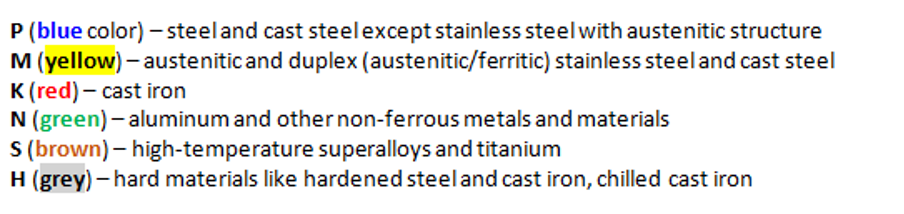
\includegraphics[width=4.166667in, keepaspectratio=true]{./ZimFiles_files/Verslagen/Activiteiten_rapport/Activities/Masterproef_Tool_Wear_Inspection_-_Meeting3_TJ/Types_sterkte_plaatjes.png}
	
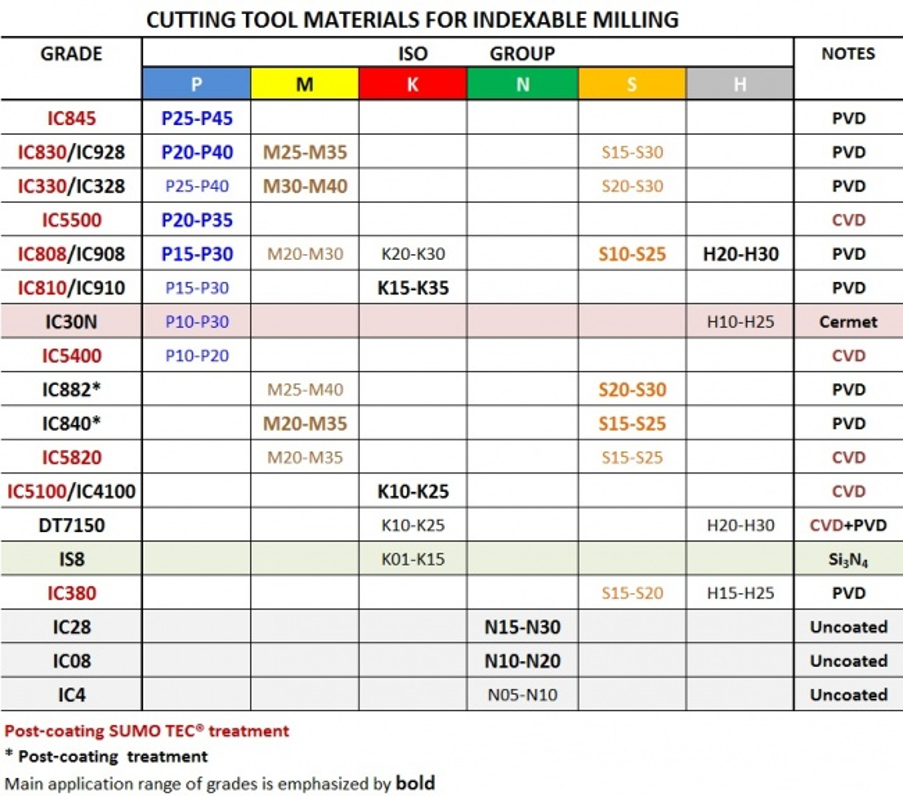
\includegraphics[width=4.166667in, keepaspectratio=true]{./ZimFiles_files/Verslagen/Activiteiten_rapport/Activities/Masterproef_Tool_Wear_Inspection_-_Meeting3_TJ/plaatjes_nummers.png}



Wat slijt er af?

	Is het afgesleten wanneer de coating weg is
	
		Coating slijt eerst af, daarna wordt het materiaal binnenin afgesleten
		
	Of wordt er gewoon een stukje van de coating afgesleten
	


De nauwkeurigheid van de frees -\textgreater{} om te vergelijken met de stappenmotor die op 0,106° nauwkeurig zal bewegen 

	Niet indexeerbaar of te draaien, desnoods uit frees nemen en in houder zetten om de foto te nemen, dus zelf ook niet te nauwkeurig werken.
	
	





Heeft u enkele voorbeelden van de verschillende slijtage types van de plaatjes?

	4 hoofd klassen, moeilijk om van allemaal een voorbeeld te vinden
	




Hoe ver moet gekeken worden op de kop en op de zijkant?

	Op de hoek zal steeds de slijtage zichtbaar zijn.
	
	

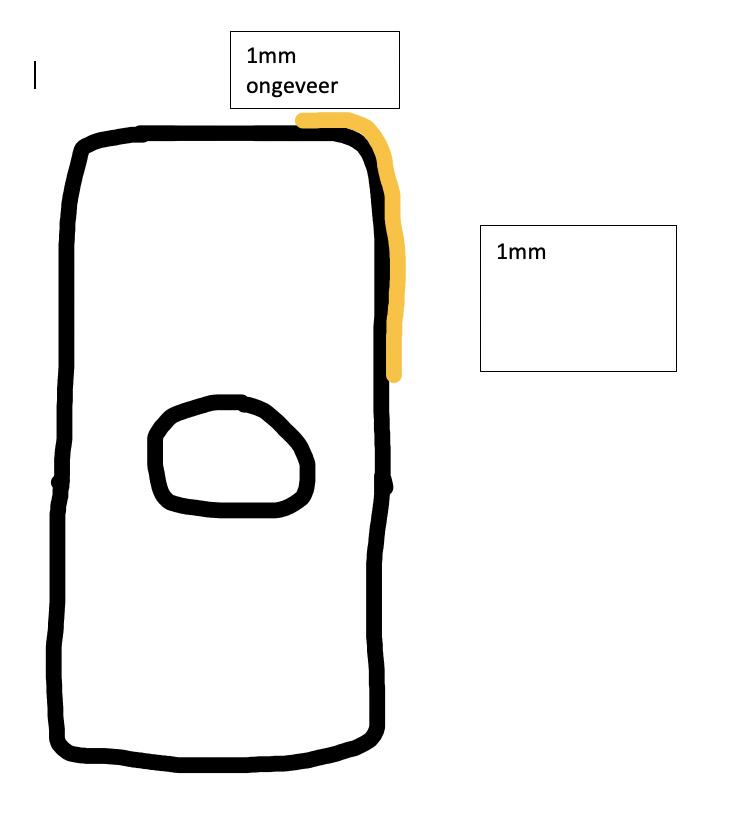
\includegraphics[width=4.166667in, keepaspectratio=true]{./ZimFiles_files/Verslagen/Activiteiten_rapport/Activities/Masterproef_Tool_Wear_Inspection_-_Meeting3_TJ/Screenshot 2020-11-20 at 15.20.56.png}



Extra metric toevoegen die de oppervlakte geeft van de fout, niet enkel de afstand die gegeven is voor test set. 

Gewoon lichte pixels berekenen






		\section{Masterproef Tool Wear Inspection - Update 1 DH}

Created vrijdag 20 november 2020





\subsection{Mail:}

Beste meneer Hulens,

 

Ik ben vorige week langsgegaan bij Tom Jacobs van Sirris om de eerste testplaatjes te gaan halen en heb afgesproken dat hij de volgende 200 gelabelde plaatjes kan klaarleggen tegen het einde van de maand.

Aansluitend ben ik ook gaan kijken naar de visie opstelling van Robbert bij het staalverwerkingsbedrijf Aperam waar fouten worden gedetecteerd op grote staalplaten die daar geproduceerd worden.

 

Nu ben ik bezig met het formuleren van de beschrijving van het probleem en het verleden te beschrijven. Ik vind het hier lastig om gestart te geraken en mijn weg te vinden in de hoop papers en boeken. Stilaan begin ik wel een methode te vinden om de bronnen gestructureerd te kunnen overlopen en documenteren.

 

Aan de implementatie heb ik niet meer zo heel veel gedaan. Ik heb een regressie model proberen opzetten met de Keras library, maar dat had weinig resultaat gezien Keras eigenlijk geen ondersteuning bied voor regressie problemen. Mijn volgende stap hierbij is PyTorch gebruiken en testen of dit hier wel makkelijker gaat. Keras liet ook niet toe mijn labels correct door te geven voor het classificatie model met meer dan twee klassen. Ik hoop dit ook verder uit te kunnen werken gezien Tom aangaf dat er wel degelijk een drempelwaarde van slijtage is waarbij de plaatjes moeten vervangen worden. Zo zal ik drie klassen maken: {“goed”, “bijna te vervangen”, “te vervangen”}.

Hij vertelde ook dat de plaatjes die nu gegeven worden niet door een machine gesleten worden, maar gewoon met een vijl. Hierdoor zijn de verschillende soorten slijtage niet zichtbaar. Ik het tweede semester zag hij het wel zitten om een aantal plaatjes te voorzien die wel door de machines gesleten zijn om daarop de slijtage types te herkennen.

 

Mijn planning schrijft voor om op 29/10 te starten met de uitwerking van een testopstelling, kan u tegen dan een microscoop camera voorzien en/of moet ik hiervoor verder zelf nog iets in orde brengen?

 

Ter info geef ik hier mijn notities nog mee die ik heb opgeschreven tijdens de afspraak met Tom Jacobs:

Tegen eind oktober 200 extra plaatjes

Na nieuwjaar kijken hoeveel “echte” plaatjes nodig zijn om de soorten slijtage op te kunnen bepalen

Nauwkeurigheid die gehaald zou moeten worden is 20 micrometer

Plaatje is slecht vanaf het een slijtage heeft van meer dan 200 micrometer (best iets vroeger kunnen zeggen dat het plaatje de grens van 200 micron zal overschrijden)

Hoe de inspectie nu gebeurt:

Uithalen en bekijken met blote oog of lens

Elke vaste tijdspan verwisselen

Maandelijkse update om vooruitgang te bespreken

Verschillende coatings moeten ook onderzocht worden

Kostprijs mee bekeken voor de hele setup

 

Met vriendelijke groeten,

 

Lars De Pauw



\subsection{Reply}

Beste Lars,



Zeer goed dat je de plaatjes hebt. Ik bestelde zojuist ook een nieuwe microscoopcamera waarmee je aan de slag kan.



Heeft het bezoek aan Aperam geholpen om ideeen op te doen voor jou toepassing? Misschien gebruiken ze speciale belichting ofzo om de fouten te accentueren?



Bij het beschrijven van je probleem zou ik zoeken naar technieken om abnormaliteiten te detecteren. Als je er een aantal gevonden hebt die voor voor jou interessant zijn is dat oke. Je moet er nu geen 10tallen opsommen. Wat ook interessant is zijn belichtingstechnieken om de fout duidelijker in beeld te brengen, maar ik weet niet of je daar veel over gaat vinden.



 Kan je toevallig volgende woensdag om 13u naar de campus komen? Dan ben ik daar ook en kan ik je de camera geven + even bespreken?



Mvg,



Dries Hulens



\subsection{Mail:}

Beste meneer Hulens,



Bij Aperam is de schaal wat anders en wordt een bewegende plaat gefotografeerd, dat geeft een heel verschil. Daar worden de camera en belichting op 45graden opgesteld tenopzichte van de plaat. Door de hoge fps van de camera (1000Hz) wordt een ander type belichting gebruikt om de 50Hz belichting te verbergen. Dit zal ook niet meteen van toepassing zijn bij dit onderzoek lijkt me. Ik ben wel een aantal papers tegengekomen waar men gebruikmaakt van fluorescentie lampen voor de belichtingen. Dat moet ik nog onderzoeken wat daar de voordelen van zouden zijn.



De technieken die ik tot nu toe vond zijn vooral gebaseerd op het zelf beschrijven van een model in plaats van deep learning te gebruiken. Wel was er een interessante studie die een 3D laser gebruikte in plaats van een camera waarbij zeer goede resultaten bereikt werden. 

De belichting ga ik zeker eens opzoeken wat daarvoor nodig is en wat de beste resultaten zou geven op die schaal. 



Volgende week woensdag 21/10 om 13 uur is in orde. Ik hoop tegen dan een nieuwe implementatie te kunnen tonen van het regressie model.



Met vriendelijke groeten,



Lars De Pauw


		\section{Masterproef Tool Wear Inspection - Update 2 DH}

Created vrijdag 20 november 2020



\subsection{Mail}

Beste meneer Hulens,

 

Een nieuwe update over mijn masterproef over Tool Wear Inspection.

Hieronder een overzicht van wat ik heb gedaan, wat ik zal doen en een korte samenvatting van wat we vorige keer hebben besproken.

 

Wat ik afgelopen week heb gedaan:

Opstelling maken

Een simpele setup bepalen om snel te zien wat de plaatjes doen met het invallende licht en hoe dit op de camera overkomt. Hierbij kwam ik al op vrij goede resultaten voor de belichting door een bureaulamp horizontaal te laten schijnen op het plaatje. Hier is een foto van te vinden in de bijlage. Hier staat ook het licht van de camera nog aan, wanneer dit wordt uitgeschakeld is de fout mooi in het oranje te zien en is de achtergrond vrij donker (te zien in bijlage).






\includegraphics[width=4.166667in, keepaspectratio=true]{./ZimFiles_files/Verslagen/Activiteiten_rapport/Activities/Masterproef_Tool_Wear_Inspection_-_Update_2_DH/eerste-opstelling_donkere_achtergrond3.jpg}




Begin van een setup met een rad waar 20 plaatjes op gemonteerd kunnen worden. Hiervoor heb ik al een 3D model geprint en ben ik gestart aan de aansturing van de motor. Voor de motor heb ik ook berekend dat ik nog een stapreductie zal moeten doen van ongeveer 4:1 gezien een stap van de motor die ik heb (NEMA17) momenteel 1,7mm bedraagt op de rand van het rad. Dit wil ik hiermee terugbrengen tot 0,4mm zodat de plaatjes nauwkeurig voor de camera geplaatst kunnen worden. Ik dacht hiervoor een set van tandwielen zelf te 3D printen. Een foto van de opstelling is te zien in de bijlage.

A close up of a device



\includegraphics[width=4.166667in, keepaspectratio=true]{./ZimFiles_files/Verslagen/Activiteiten_rapport/Activities/Masterproef_Tool_Wear_Inspection_-_Update_2_DH/radhouder_horizontal.jpeg}

Bekijken welke lichten beschikbaar zijn.

Lange stevige led strips wit licht van ongeveer 30cm. Deze kunnen worden aangestuurd met een relais vanaf de raspberry pi, maar met mijn Solid State relais gaf dit een zeer vreemd gedrag. Bij het uitschakelen bleven de leds gewoon branden en was er een weerstand te meten van enkele mega Ohm. Daarom heb ik geprobeerd met een gewone aanstuurbare relais en dit werkte wel, maar hier heb ik er slechts één van. Ik heb nog een andere opstelling voor deze ledstrips getest door transistoren te gebruiken als switch, maar hier denk ik de foute transistoren gebruikt te hebben. Daar heb ik geen verdere berekeningen rond gedaan gezien dat niet het doel is van het onderzoek. Daarom mijn vraag: zijn er enkele (3) relais beschikbaar op de campus die ik zou kunnen gebruiken of kunnen er eventueel besteld worden? Ik heb er indien nodig zelf 3, maar dan moet ik die uit andere projecten halen.

De adresseerbare led strip heb ik nog niet kunnen testen.

Documenteren van alle afgelopen tests en opstellingen in zim (uitgezonderd software). Dit is allemaal geschreven in het engels om mezelf te verplichten om wat meer na te denken over de woorden en zinnen in het engels om later vlotter te kunnen schrijven aan de thesis tekst.

De Zim bestanden staan publiek op github: \href{https://github.com/dplars/TWI_zim.git}{https://github.com/dplars/TWI\_zim.git}

Is het voor u handig om de zim notebook zelf te openen of stuur ik hier best een samenvatting van?

 

Wat ik komende week zou willen doen:

Langsgaan bij Tom Jacobs voor de extra 300 plaatjes en enkele vragen.

De opstelling met het rad afronden voor de camera en de plaatjes zonder belichting.

De invloed van de lichtkleur op de plaatjes onderzoeken als ik weet uit welke materialen de plaatjes bestaan en of de plaatjes allemaal uit hetzelfde materiaal bestaan.

 

Wat we vorige keer hadden besproken:

Opstelling

3D printen

Verschillende kanten belichten en in channels van de foto zetten

Wanneer de fouten die voorkomen in de plaatjes gekend zijn beoordelen of de resolutie van de camera hoog genoeg is.

Licht

Onderzoeken of er bepaalde reacties zijn van de materialen op golflengtes

Hiervoor en voor de verschillende belichtingshoeken gebruikmaken van adresseerbare led strip

Andere punten

Vooral veel testen en goed documenteren, het echte schrijven komt later pas

Een binair classificatie model gebruiken om de verschillende camera setups snel te kunnen testen.

Eventueel de grootste reflectie blob uitsnijden om de achtergrond weg te kunnen werken.

 

Herhaling van de vragen:

Zijn er 3 relais beschikbaar om de lichten mee te kunnen aansturen?

Zim delen via github of een samenvatting geven?

 

 

Met vriendelijke groeten,

 

Lars De Pauw



\subsection{Reply}

Beste Lars,



Dat ziet er al zeer goed uit! Als we met bepaalde kleuren gaan werken kunnen we de slijtage ook nog beter afzonderen van de rest van de foto.



Als je wil kan ik je relais opsturen maar ik zou eerder opteren om de ledstrips met mosfets te schakelen om dat klikgeluid niet altijd te hebben. Die kan ik ook bij jou laten leveren als je wil? Laat maar weten wat voor jou het beste lijkt.



Het rad ziet er ook zeer goed uit! In fusion360 heb je plugins voor tandwielen te genereren, welk tekenprogramma gebruik je juist?



Ik ben benieuwd als je de plaatjes op het rad zet en ze voorbij de camera laat draaien of de hoek van het licht dan perfect is voor elk plaatje, of dat je onder verschillende hoeken moet belichten. Maar dat kunnen we dan zien als die setup up and running is.



Goed bezig en succes!



\subsection{Mail}

Beste meneer Hulens,

 

Ik heb intussen nog mosfets gevonden thuis en kan de leds hiermee aansturen.

 Fusion 360 is inderdaad gebruikt geweest om de 3D modellen te tekenen. Echter heb ik na het testen gemerkt dat ik de motordriver driver kan instellen om tot 1/16 van een stap te bewegen, waardoor de tandwielen niet meer nodig zijn.

 

De testopstelling is bijna klaar nu, enkel nog de camera monteren en dan kan ik beginnen kijken naar het effect van het licht op de beelden.

 

Woensdag heb ik afgesproken met Tom Jacobs, hij kan nog 90 gelabelde plaatjes (180 snijkanten) voorzien.

 

Met vriendelijke groeten,

 

Lars De Pauw


		\section{Masterproef Tool Wear Inspection - Update 3 DH}

Created vrijdag 20 november 2020



\subsection{Mail}

Beste meneer Hulens,

 

Ik heb mijn eerste beeldjes kunnen maken met het geautomatiseerd systeem.

Een foto van de opstelling die ik nu gebruik zit in bijlage, hierbij zijn er twee bogen waarop een enkel adresseerbare ledstrip is geplaatst. De ene boog kan nog vrij draaien om de hoek tussen de twee ledstrips aan te passen.



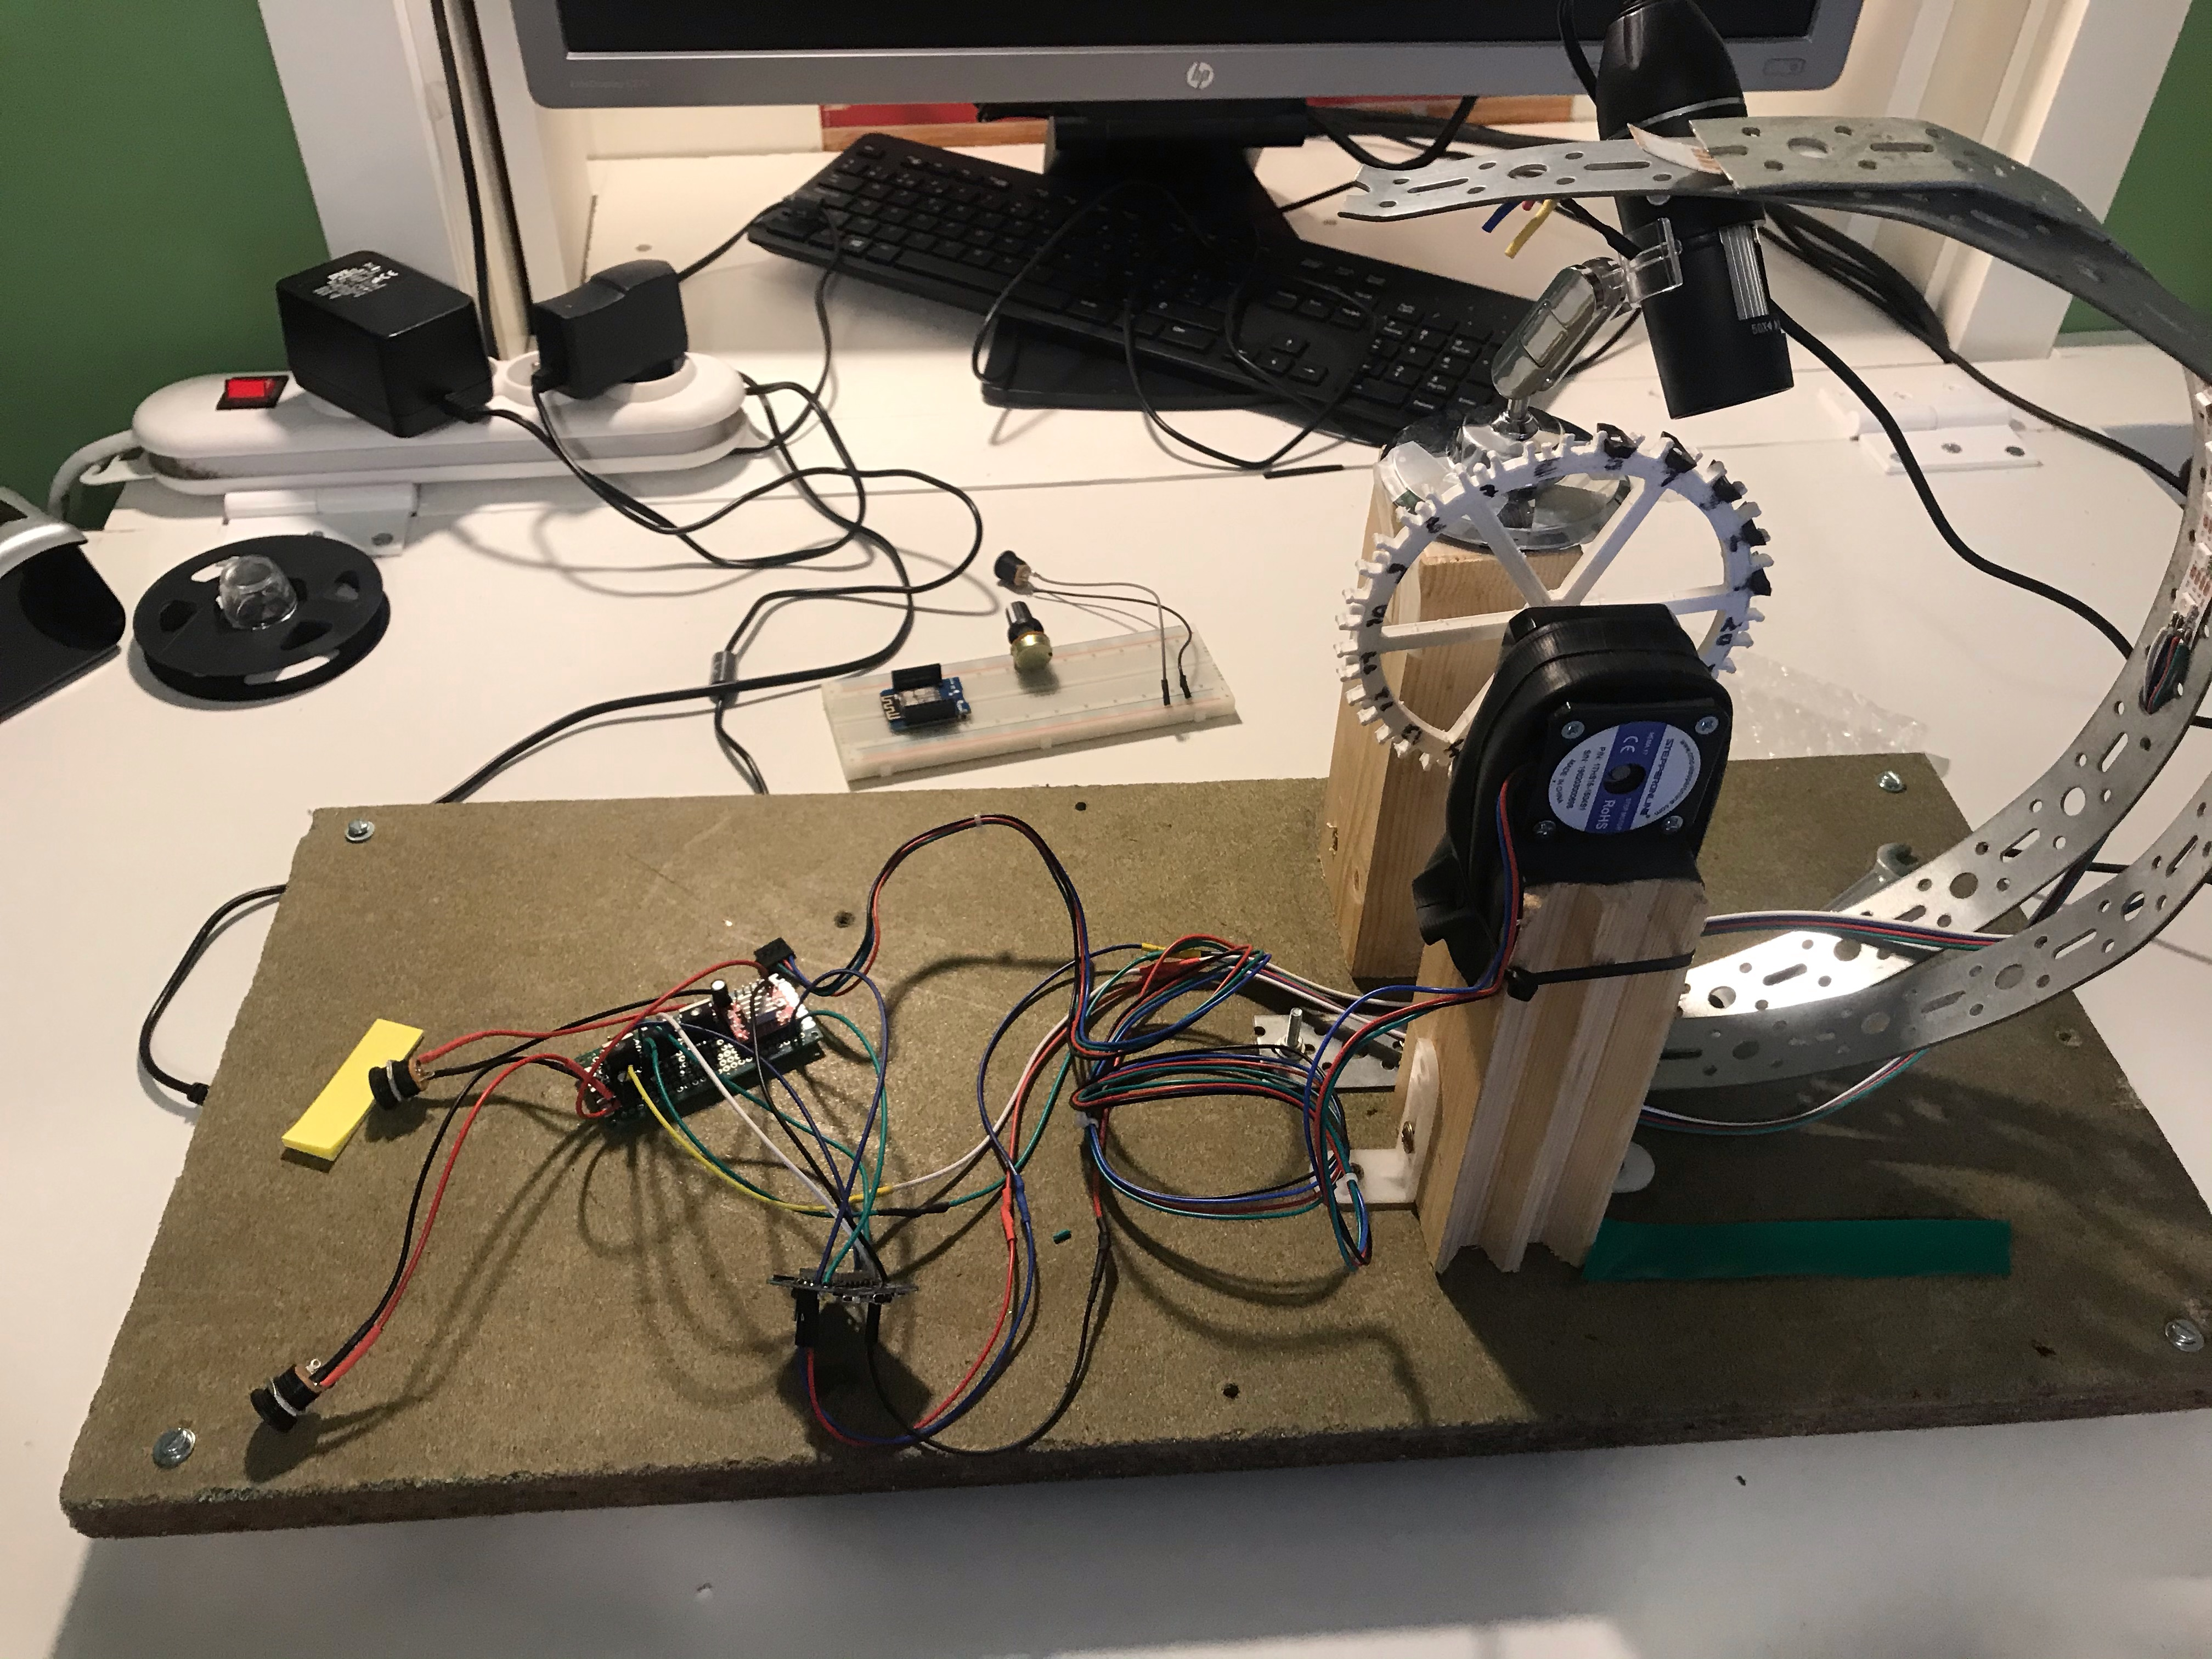
\includegraphics[width=4.166667in, keepaspectratio=true]{./ZimFiles_files/Verslagen/Activiteiten_rapport/Activities/Masterproef_Tool_Wear_Inspection_-_Update_3_DH/rechts_kabels.jpeg}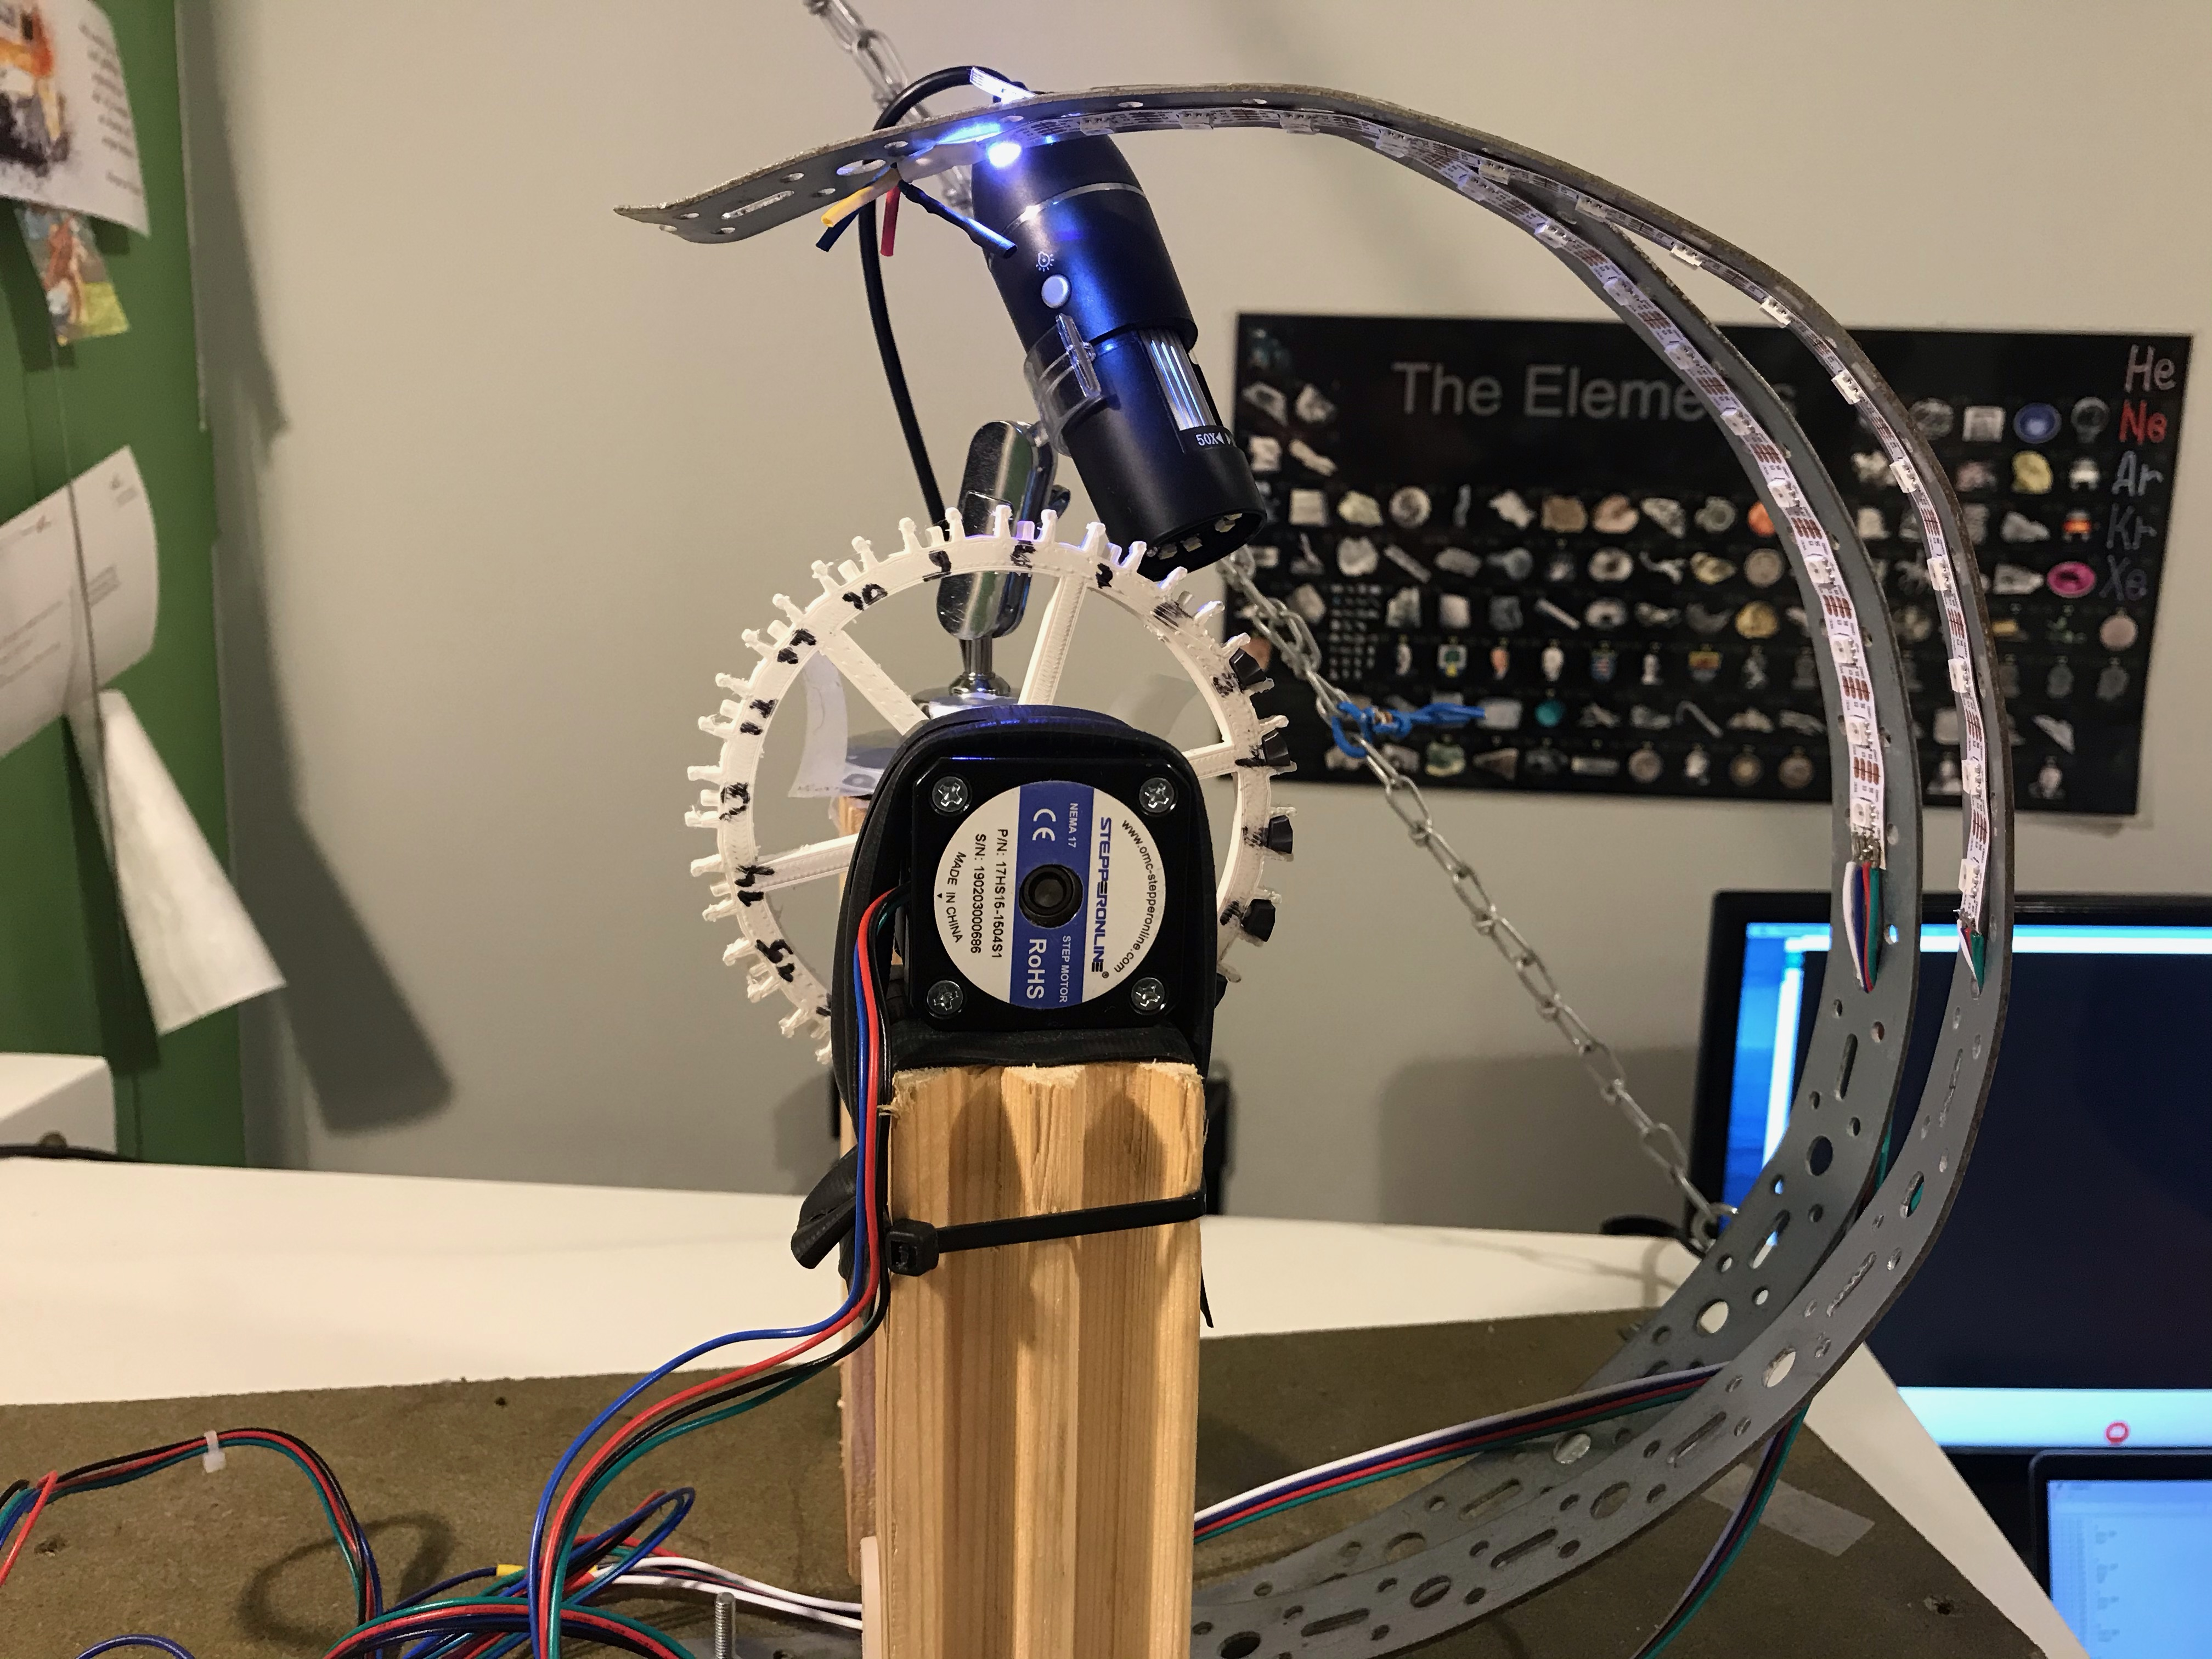
\includegraphics[width=4.166667in, keepaspectratio=true]{./ZimFiles_files/Verslagen/Activiteiten_rapport/Activities/Masterproef_Tool_Wear_Inspection_-_Update_3_DH/rechts.jpeg}

 

Enkele genomen foto’s zitten in bijlage, ik heb hier telkens een foto genomen wanneer twee overeenkomstige leds van de ledstrips branden en al de rest uit om te zien welke leds overeenkomen met welke weerkaatsing in de camera. Op de foto’s is mooi te zien hoe elke led een ander deel van de slijtage belicht.

A picture containing dark, sitting, looking, lit



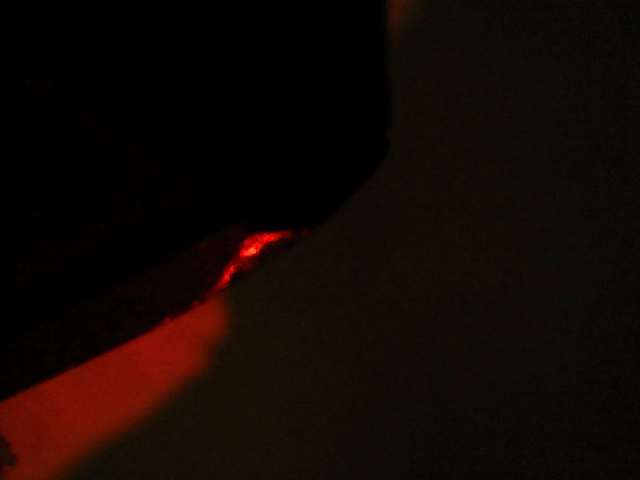
\includegraphics[width=4.166667in, keepaspectratio=true]{./ZimFiles_files/Verslagen/Activiteiten_rapport/Activities/Masterproef_Tool_Wear_Inspection_-_Update_3_DH/p4_l10.png}\includegraphics[width=4.166667in, keepaspectratio=true]{./ZimFiles_files/Verslagen/Activiteiten_rapport/Activities/Masterproef_Tool_Wear_Inspection_-_Update_3_DH/p4_l9.png}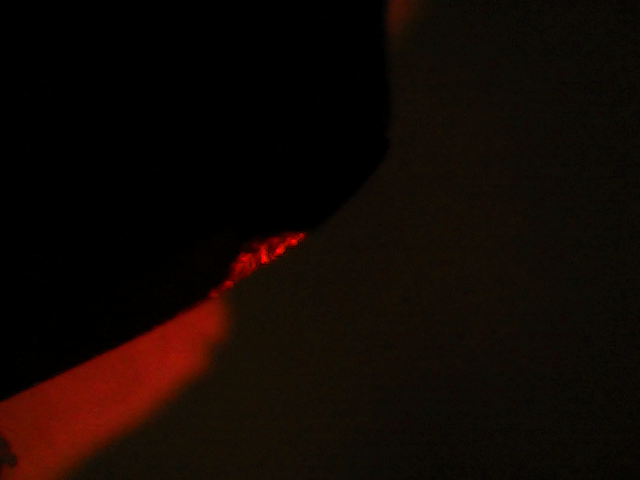
\includegraphics[width=4.166667in, keepaspectratio=true]{./ZimFiles_files/Verslagen/Activiteiten_rapport/Activities/Masterproef_Tool_Wear_Inspection_-_Update_3_DH/p4_l8.png}\includegraphics[width=4.166667in, keepaspectratio=true]{./ZimFiles_files/Verslagen/Activiteiten_rapport/Activities/Masterproef_Tool_Wear_Inspection_-_Update_3_DH/p4.png}

 

Hier lijkt de belichting dus wel goed te zitten, maar is er nog licht weerkaatsing van de witte houder waarin de plaatjes zitten. Om dit weg te werken dacht ik er aan om ofwel het rad met zwart filament te printen of het witte rad zwart te verven, ik hoop dat dat de problemen zou oplossen. De andere optie is om er voor te zorgen dat de houder in de schaduw ligt. Dat is echter wat moeilijker gezien de twee ledstrips van een andere hoek belichten.

 

Om de leds en de motor aan te sturen werk ik met een python programma dat via pyserial gegevens doorstuurt naar een Wemos D1 mini, die met de software van arduino werkt, door op zijn poort te schrijven. Dit ging echter heel traag waardoor ik na elk commando 1,5 seconden moest wachten eer ik het volgende commando kon sturen of er iets anders kon gebeuren. Dat zorgde ervoor dat elke foto ongeveer 5 seconden duurde. Dit met 15 verschillende licht settings was niet ideaal dus ik ga de communicatie snelheid nog proberen verhogen en anders een echte arduino gebruiken in de hoop dat dat sneller werkt.

 

De reden dat ik het via deze omslachtige manier doe (via seriele poort naar een arduino) is omdat ik heb geprobeerd om met een raspberry pi alles uit te voeren, aansturing van de leds en de beeld opname, maar dat ging ook vrij traag.

En er is een raspberry pi stuk gegaan door een kortsluiting in het pcb dat ik had gesoldeerd. Om niet nog een raspberry pi kapot te maken ben ik overgeschakeld naar de Wemos D1 mini chips die veel minder duur zijn, wat de gevolgen van een kortsluiting een heel stuk beperkt.

 

Ik heb ook opgezocht of het wolfram carbide waaruit de plaatjes zijn gemaakt bepaalde reflectieve eigenschappen heeft, maar dit was zonder succes. Er waren wel een aantal studies die de licht absorbtie besproken om fouten te herkennen en die lagen vooral in het infrarode spectrum. De echte reflectiviteit zal ik misschien eens proef ondervindelijk moeten uitzoeken.

 

Met vriendelijke groeten,

 

Lars De Pauw



\subsection{Reply}

Hallo Lars,



Dat ziet er al heel goed uit!​ Op de foto's kan je inderdaad duidelijk de slijtage zien. Misschien kunnen we zelf die 4 foto's combineren tot 1 foto, of als je de bijhorende 4 led's gelijktijdig laat branden, krijg je dan het zelfde resultaat? 



De weerkaatsing van de draaischijf kan je inderdaad oplossen met verf of zwart filament. 



Zeker de info bijhouden over lichtabsorbtie in het IR spectrum, dit kan je bij in u literatuurstudie zetten.



Super goed bezig! Dit gaat zeker het resultaat verbeteren, dat je al vertrekt met goede foto's!



Mvg,





\subsection{Mail}

Beste meneer Hulens,

 

Die vier foto’s zelf combineren tot één foto lijkt me de meest stabiele methode gezien de leds niet steeds hetzelfde resultaat geven voor een verschillend plaatje. In bijlage zitten twee foto’s van verschillende plaatjes die met dezelfde leds belicht zijn.



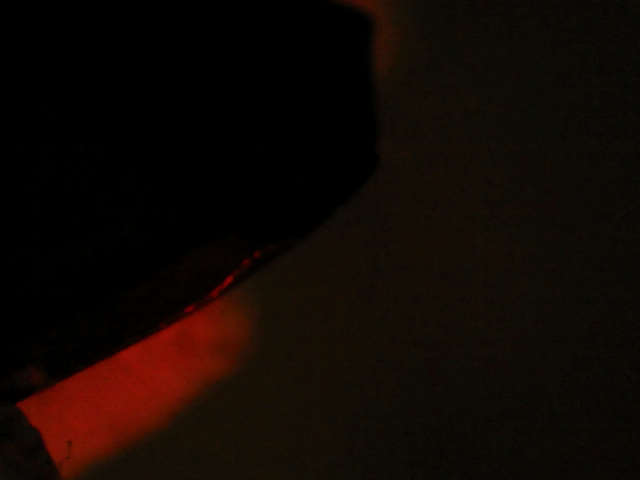
\includegraphics[width=4.166667in, keepaspectratio=true]{./ZimFiles_files/Verslagen/Activiteiten_rapport/Activities/Masterproef_Tool_Wear_Inspection_-_Update_3_DH/p3_l9.png}\includegraphics[width=4.166667in, keepaspectratio=true]{./ZimFiles_files/Verslagen/Activiteiten_rapport/Activities/Masterproef_Tool_Wear_Inspection_-_Update_3_DH/p4_l9.png}

 

Dit verschil komt doordat de plaatjes niet allemaal perfect in hun houder zitten en sommige dus een beetje schuin hangen. Dat zou kunnen opgelost worden met een verbetering van de houder en dan kan er in theorie per plaatje gewoon steeds dezelfde leds oplichten. Met de huidige plaatjes die zijn afgesleten met de hand zal dit nog niet tot perfecte resultaten komen gezien de hoek waarin het materiaal is afgesleten niet constant is. -\textgreater{} ik weet nog niet over hoeveel verschil dit gaat, het kan zijn dat dit verschil slecht 5 graden is waardoor het wel zou lukken om 4 leds tegelijk aan te zetten.

De echte plaatjes die met de machine zijn afgesleten zullen normaal gezien wel steeds dezelfde slijtage hoek hebben waardoor dat wel zou werken.

 

Met vriendelijke groeten,

 

Lars De Pauw






		\section{Masterproef Tool Wear Inspection - Update 3 TJ}

Created vrijdag 20 november 2020



\subsection{Mail}



Best Tom,

 

Zoals aan het begin van de maand besproken zou ik graag afspreken om 200 nieuwe gelabelde plaatjes te komen ophalen.

Hierbij geef ik ook graag een update over mijn masterproef, waar ik sta en hoe de planning er op korte termijn uitziet.

 

Ik had even geleden nog een mail gestuurd met de vraag hoe de labels voor de plaatjes te onderscheiden zijn, wat is de A kant en wat is de B kant? Zou u hier kort op willen antwoorden gezien dit belangrijk is wanneer ik mijn foto’s ga testen.

 

Om de extra plaatjes te komen ophalen ben ik beschikbaar op volgende dagen steeds tussen 10:00 uur en 18:00 uur:

Maandag 02/11

Woensdag 04/11

Vrijdag 05/11

Woensdag 11/11

Vrijdag 13/11

 

Wanneer zou dit voor u passen?

 

Momenteel ben ik volop aan het werken aan een testopstelling die op een relatief snelle manier veel verschillende datasets kan genereren. Hierbij zijn een aantal belichtingsmogelijkheden en verschillen in camera posities die moeten kunnen getest worden op een heel aantal plaatjes om een resultaat te kunnen zien.

Om geautomatiseerd foto’s te kunnen nemen heb ik een rad ge-3D-print waarop de plaatjes kunnen worden vastgeklikt. Dit wordt dan aangestuurd met een stapmotor om 20 plaatjes in één batch te kunnen fotograferen. Zo kan de belichting en de camera vast blijven staan en zijn het de plaatjes die bewegen wat de hele opstelling vergemakkelijkt.

 

Vorige week heb ik ook een microscoopcamera ter beschikking gekregen en daar al wat beelden mee gemaakt. Hieronder/in bijlage zijn hiervan foto’s te zien. Op de eerste foto is een plaatje te zien met een grote slijtage, te tweede van een met zeer weinig slijtage. Hier is te zien dat met een juiste belichting de fout heel mooi naar voor komt. De resultaten van de software zullen nog even uitblijven gezien ik nu de eerste week wil focussen op de opstelling.



\includegraphics[width=4.166667in, keepaspectratio=true]{./ZimFiles_files/Verslagen/Activiteiten_rapport/Activities/Masterproef_Tool_Wear_Inspection_-_Update_3_TJ/eerste-opstelling_donkere_achtergrond3.jpg}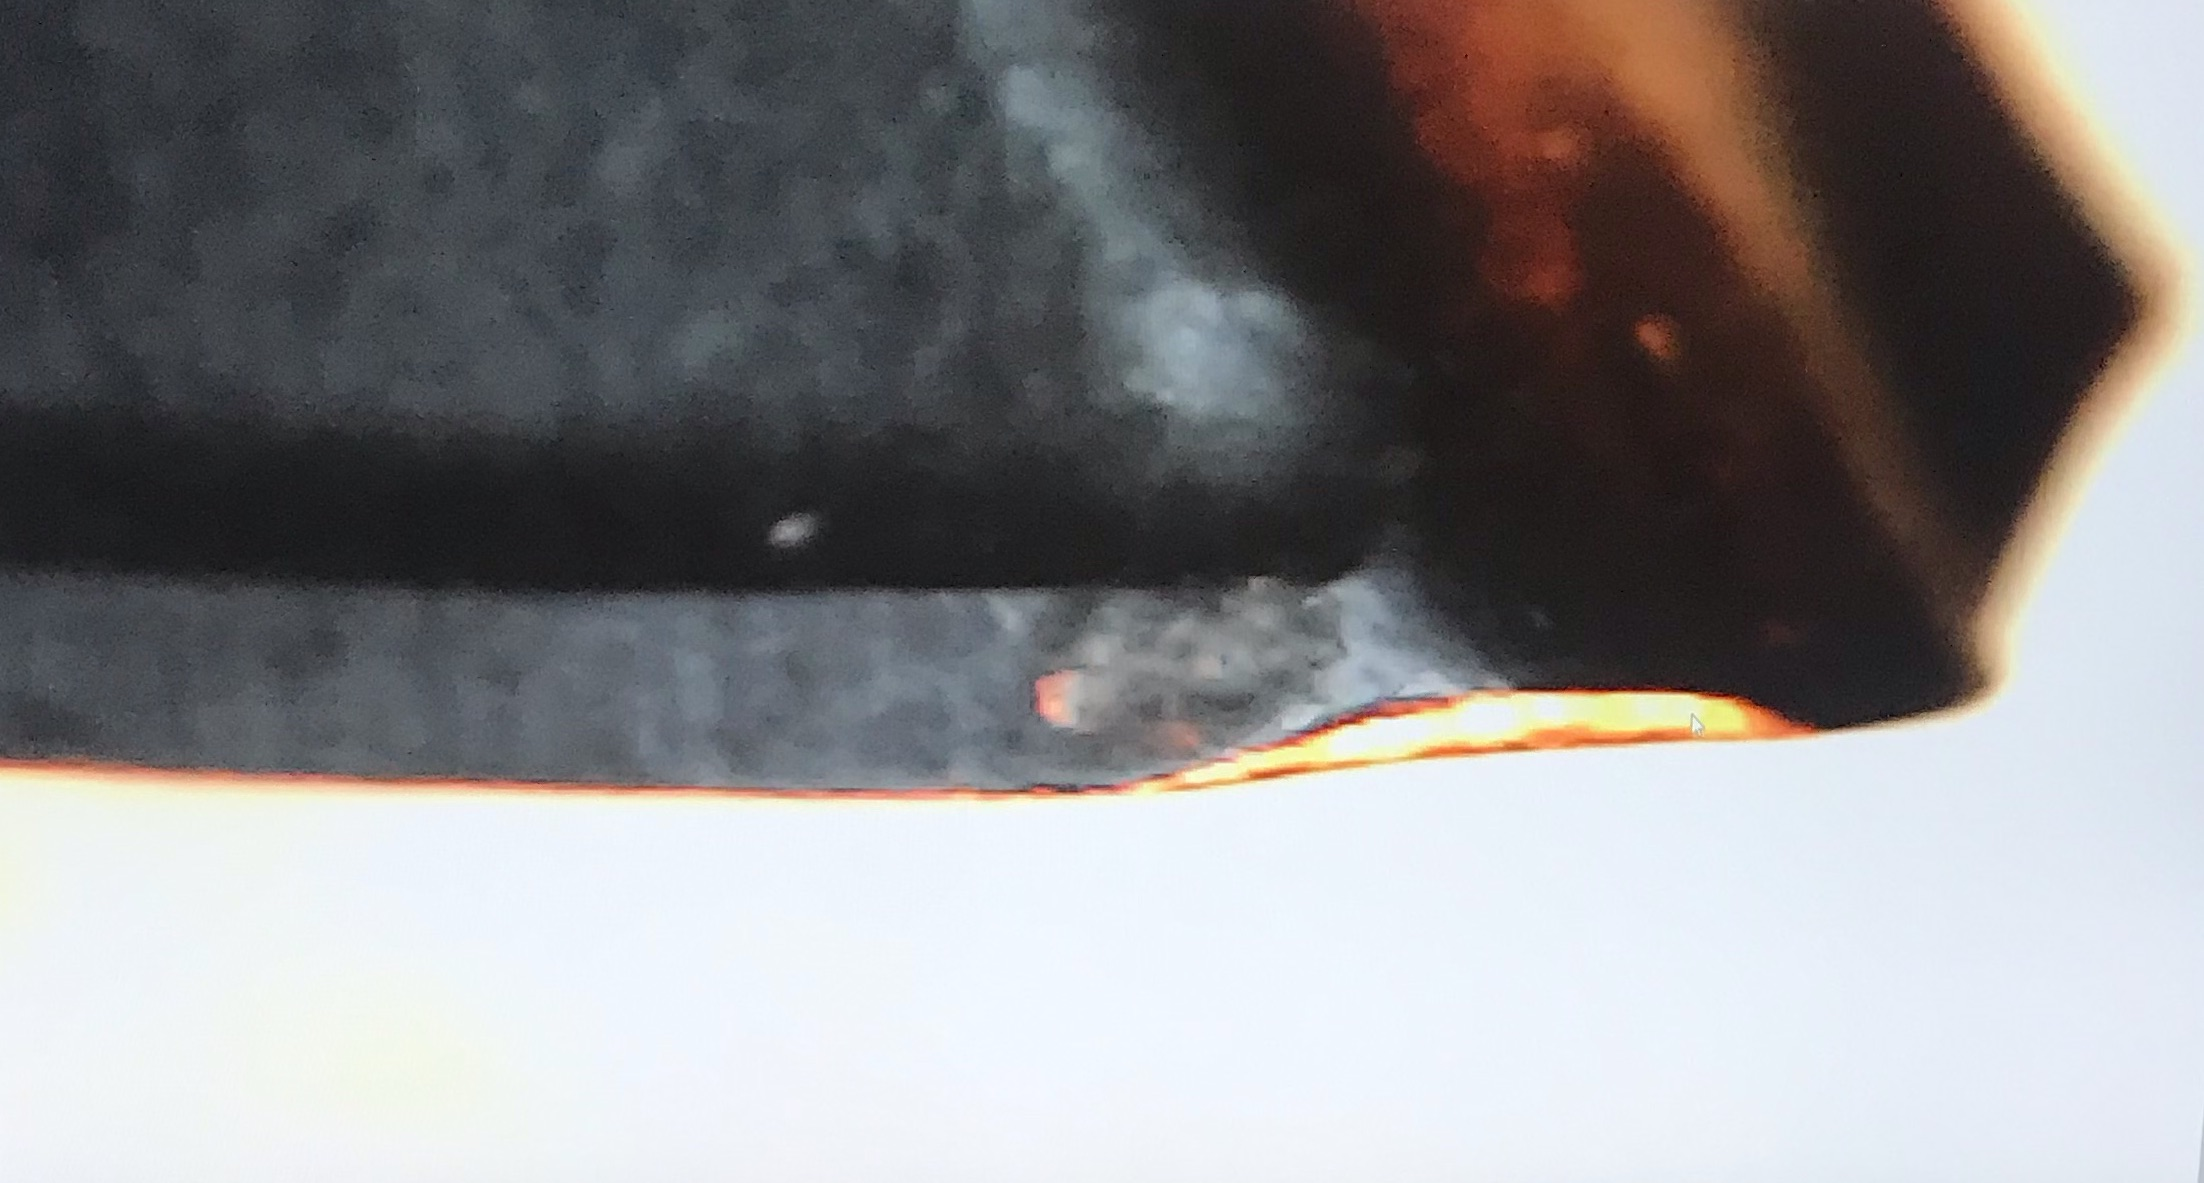
\includegraphics[width=4.166667in, keepaspectratio=true]{./ZimFiles_files/Verslagen/Activiteiten_rapport/Activities/Masterproef_Tool_Wear_Inspection_-_Update_3_TJ/eerste_setup_andere_richting_beeld2_screen image.jpeg}

 

Na de opstelling (binnen een goede week) begin ik aan een simpel algoritme dat zal bepalen of een plaatje goed of slecht is om met weinig foto’s te kunnen beslissen of een camera-opstelling goed is. Hierna kan ik met die opstelling de dataset verder uitbreiden en een algoritme maken en trainen om de effectieve fout te voorspellen in micron.

 

Met vriendelijke groeten,

 

Lars De Pauw


		\section{Masterproef Tool Wear Inspection - Update 4 DH}

Created vrijdag 20 november 2020



\subsection{Mail}

Beste meneer Hulens,

 

Ik heb intussen de problemen kunnen oplossen met de trage communicatie tussen de Arduino en de computer: de Arduino bleef 1 seconde wachten op een serial input signaal waardoor er heel veel vertraging optrad. De vertraging is nu teruggebracht tot +-1 miliseconde.

 

Echter heb ik een ander probleem, de houder die bij de camera was geleverd is onvoldoende. Deze kan niet goed genoeg vast gezet worden waardoor deze beweegt bij elke aanpassing van de setup of bij het scherpstellen van de lens. En het is hier niet makkelijk om een positie in te stellen en daar de positie van op te slaan om nadien een zelfde camera opstelling terug te kunnen maken. Liefst zou ik iets hebben waarbij de hoeken en de hoogte van de camera afleesbaar zijn of toch op een manier kwantiseerbaar.

 

Zijn er houders voorhanden op de campus? Ik denk hierbij bijvoorbeeld aan een houder van de proefbuizen van chemie?

 

Met vriendelijke groeten,

 

Lars De Pauw



\subsection{Mail}

Beste meneer Hulens,

 

Ik heb een nieuwe draaischijf geprint die de plaatjes wat beter kan vastzetten waardoor deze niet meer verschuiven en het iets makkelijker aanpasbaar is zonder het hele rad opnieuw te hoeven printen. Dit door de plaatjes vast te zetten met een clipje dat apart kan geprint worden (te zien op de foto in bijlage). Echter merk ik hier dat deze snel afbreken. Ik denk dat als ik dezelfde clipjes kan 3D printen met ABS in plaats van PLA het een stuk steviger zou worden. Dan kunnen de clipjes ook meteen in zwarte ABS geprint worden om geen licht weerkaatsing te hebben.

Ikzelf heb enkel witte PLA, moet ik dan zelf ABS bestellen of kan dat via u besteld worden? Het gaat maar over ongeveer 50 gram dus een overschot van ergens zal misschien ook al voldoende zijn.

 

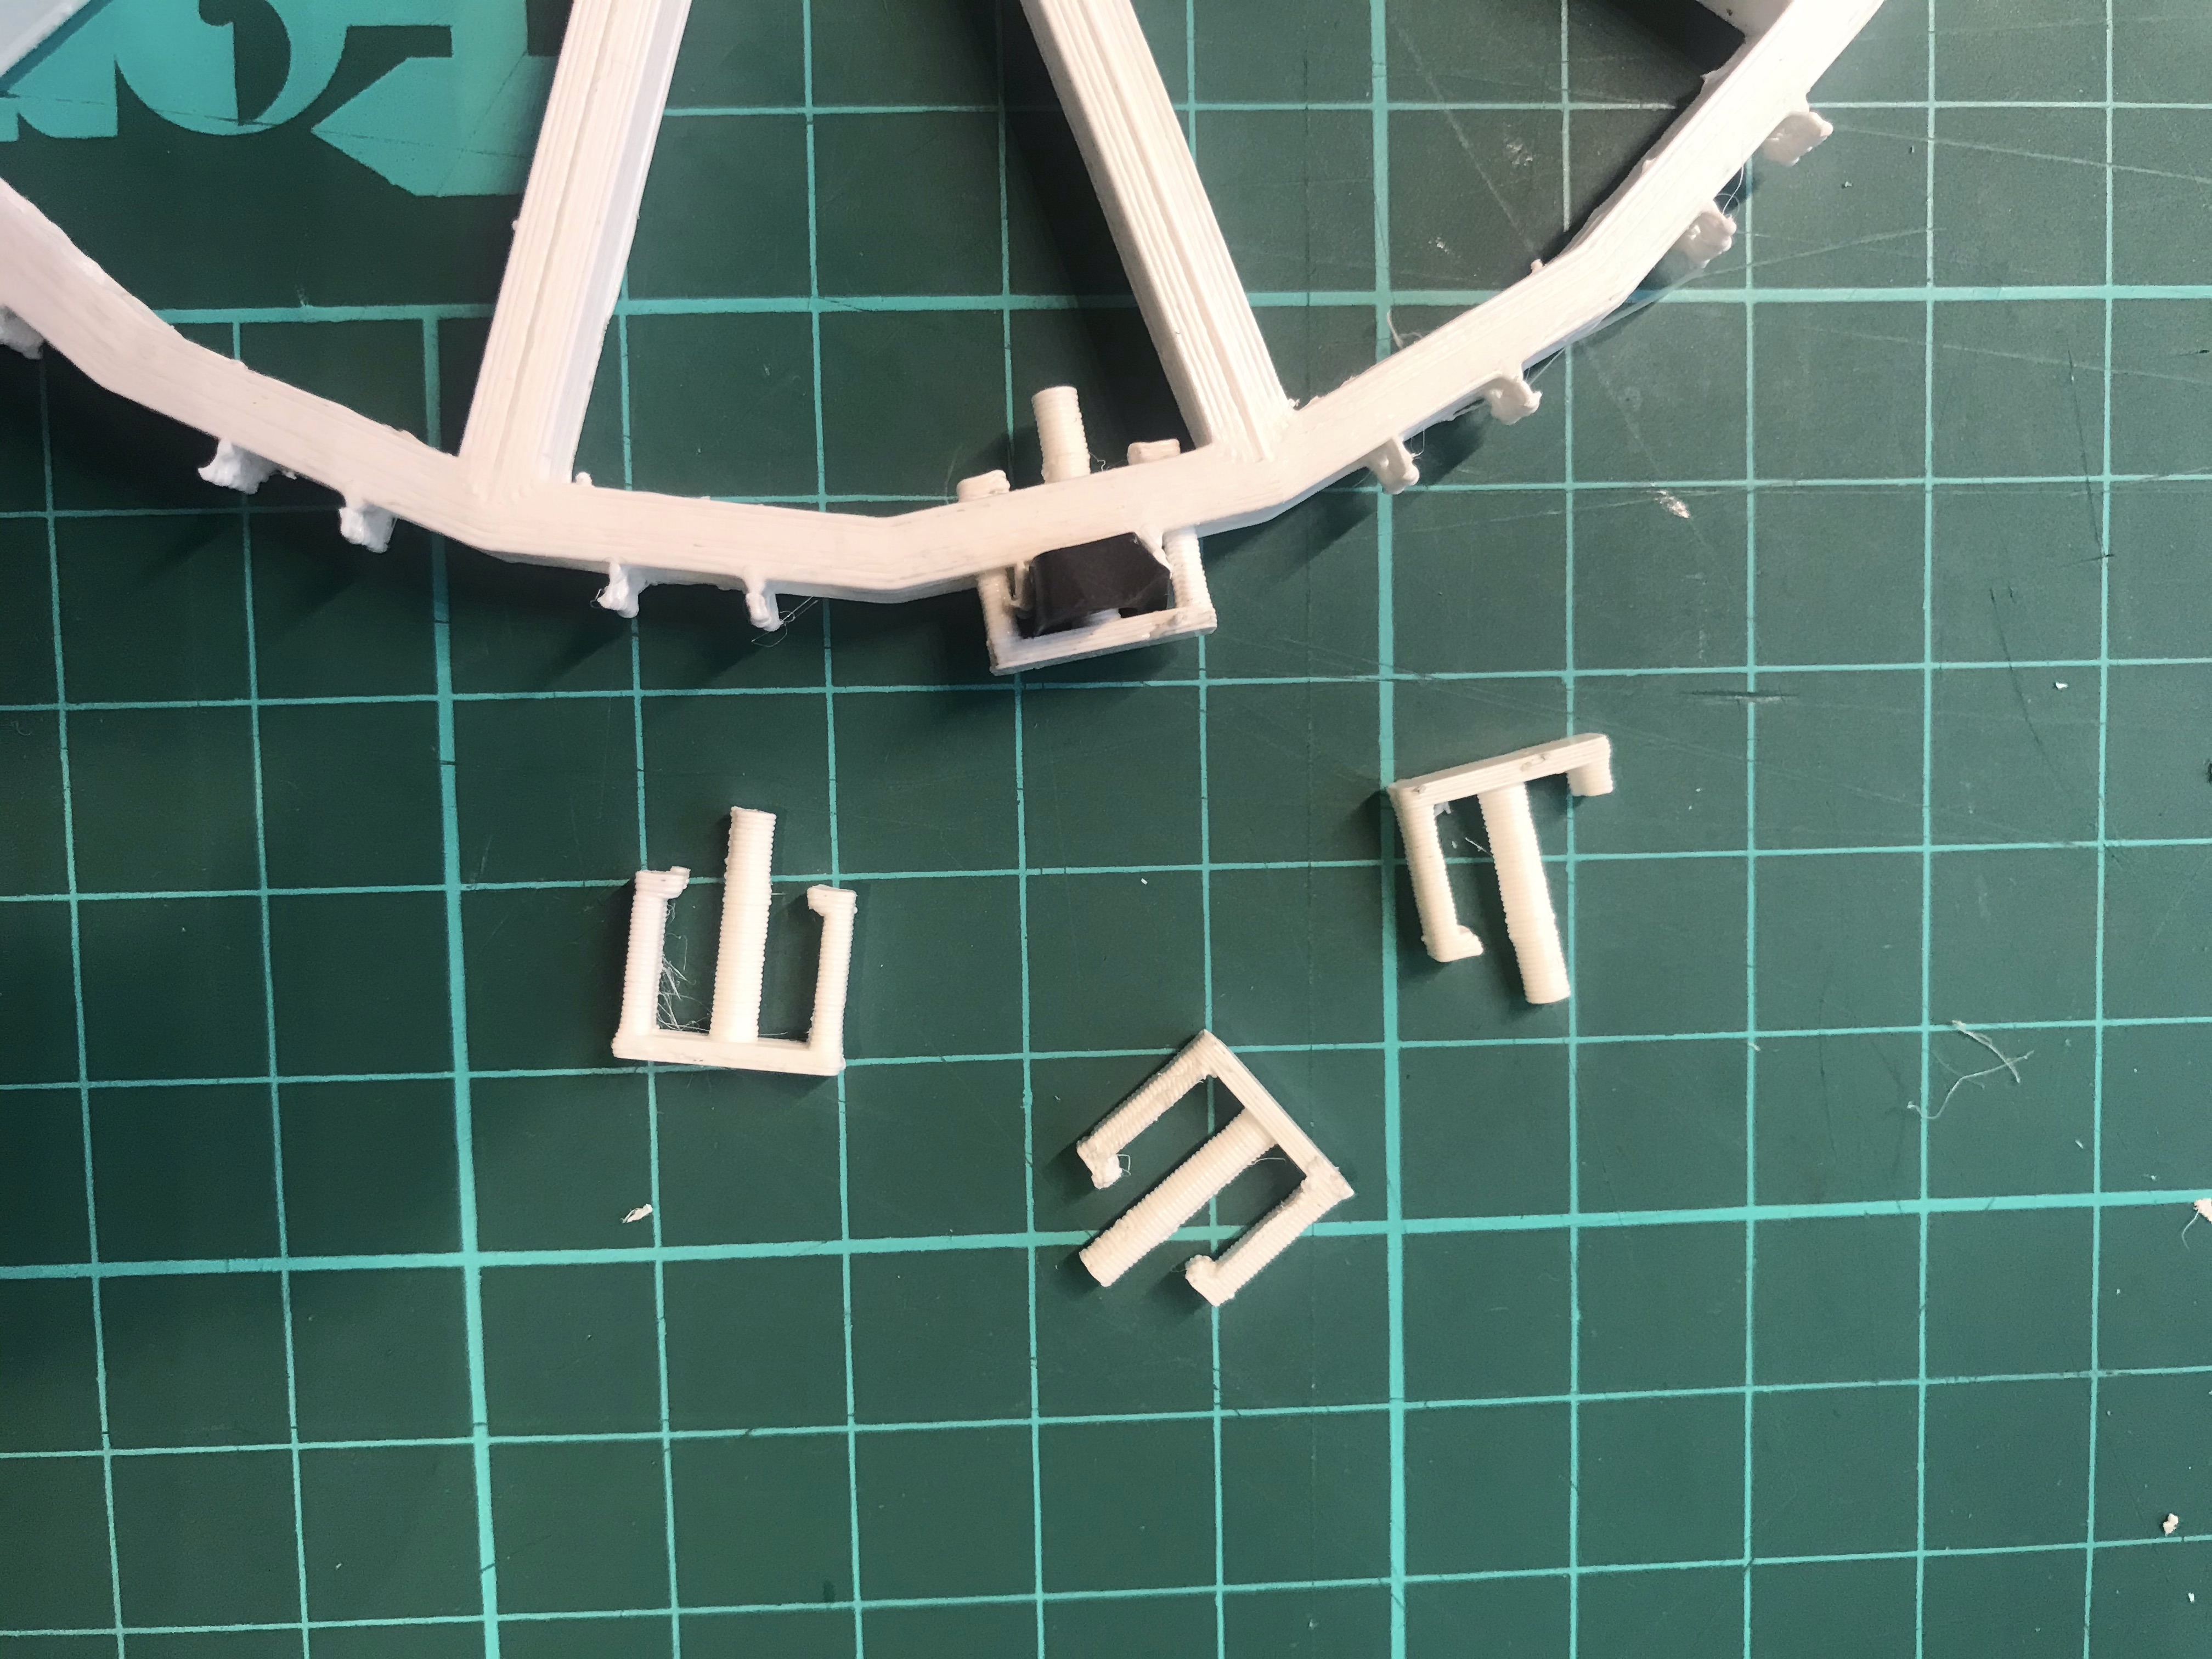
\includegraphics[width=4.166667in, keepaspectratio=true]{./ZimFiles_files/Verslagen/Activiteiten_rapport/Activities/Masterproef_Tool_Wear_Inspection_-_Update_4_DH/voorbeelden van clips op 1cm mat.jpeg}

 

Met vriendelijke groeten,

 

Lars De Pauw



\subsection{Reply}

Hallo Lars,



Ziet er zeer goed uit. Het kan ook helpen om de clips te printen zoals ze nu liggen ipv rechtopstaand. Als je wil bestel ik printmateriaal voor u. Zou het beter zijn om PETG te gebruiken voor de sterkte? Ik zal ook een aantal aluminium profielen bestellen waarmee je gemakkelijk een constructie kan maken om de camera aan te bevestigen.



Stuur me anders je adres door dan laat ik het meteen bij jou leveren.



Mvg,



\subsection{Mail}

Beste meneer Hulens,

 

De clips liggend printen zou zeker helpen voor de sterkte, maar dat zorgde er voor dat de vorm van de middelste pin niet volledig rond was. Gezien deze pin door het gat in de plaatjes moet is het hier wel belangrijk dat deze mooi rond is.

 

PETG lijkt hier inderdaad een betere optie dan ABS, die mag u zeker bestellen en laten leveren net als de aluminium profielen.

 

Het leveradres is dan:



 

Alvast bedankt!

Met vriendelijke groeten,

 

Lars De Pauw


		\section{Masterproef Tool Wear Inspection - Update 4 TG}

Created vrijdag 20 november 2020



\subsection{Mail}

Beste meneer Goedemé,

 

Ik voer de masterproef over Tool Wear Inspection uit bij Eavise in samenwerking met Sirris waarbij de slijtage van freeskop snijplaatjes gemeten moet worden.

Gezien we ongeveer in de helft van de periode tot het tussentijds verslag zitten wilde ik u als promotor graag een korte update geven over de vorderingen die reeds gemaakt zijn en wat er nog staat te gebeuren. Indien u wenst kunnen we ook eens een korte vergadering inplannen of typ ik een verslagje uit zodat ik u volledig op de hoogte kan stellen.

 

In het heel kort heb ik mij tot nu vooral bezig gehouden met het maken van een (semi geautomatiseerde) camera opstelling die per 20 snijplaatjes de nodige beelden kan maken met verschillende belichtingshoeken en verschillende kleuren belichting.

Van de plaatjes zit een foto in bijlage. Deze zijn ongeveer 0,5cm op 1cm en hebben een slijtage die met het oog nauwelijks zichtbaar is. A picture containing building, floor, sitting, table



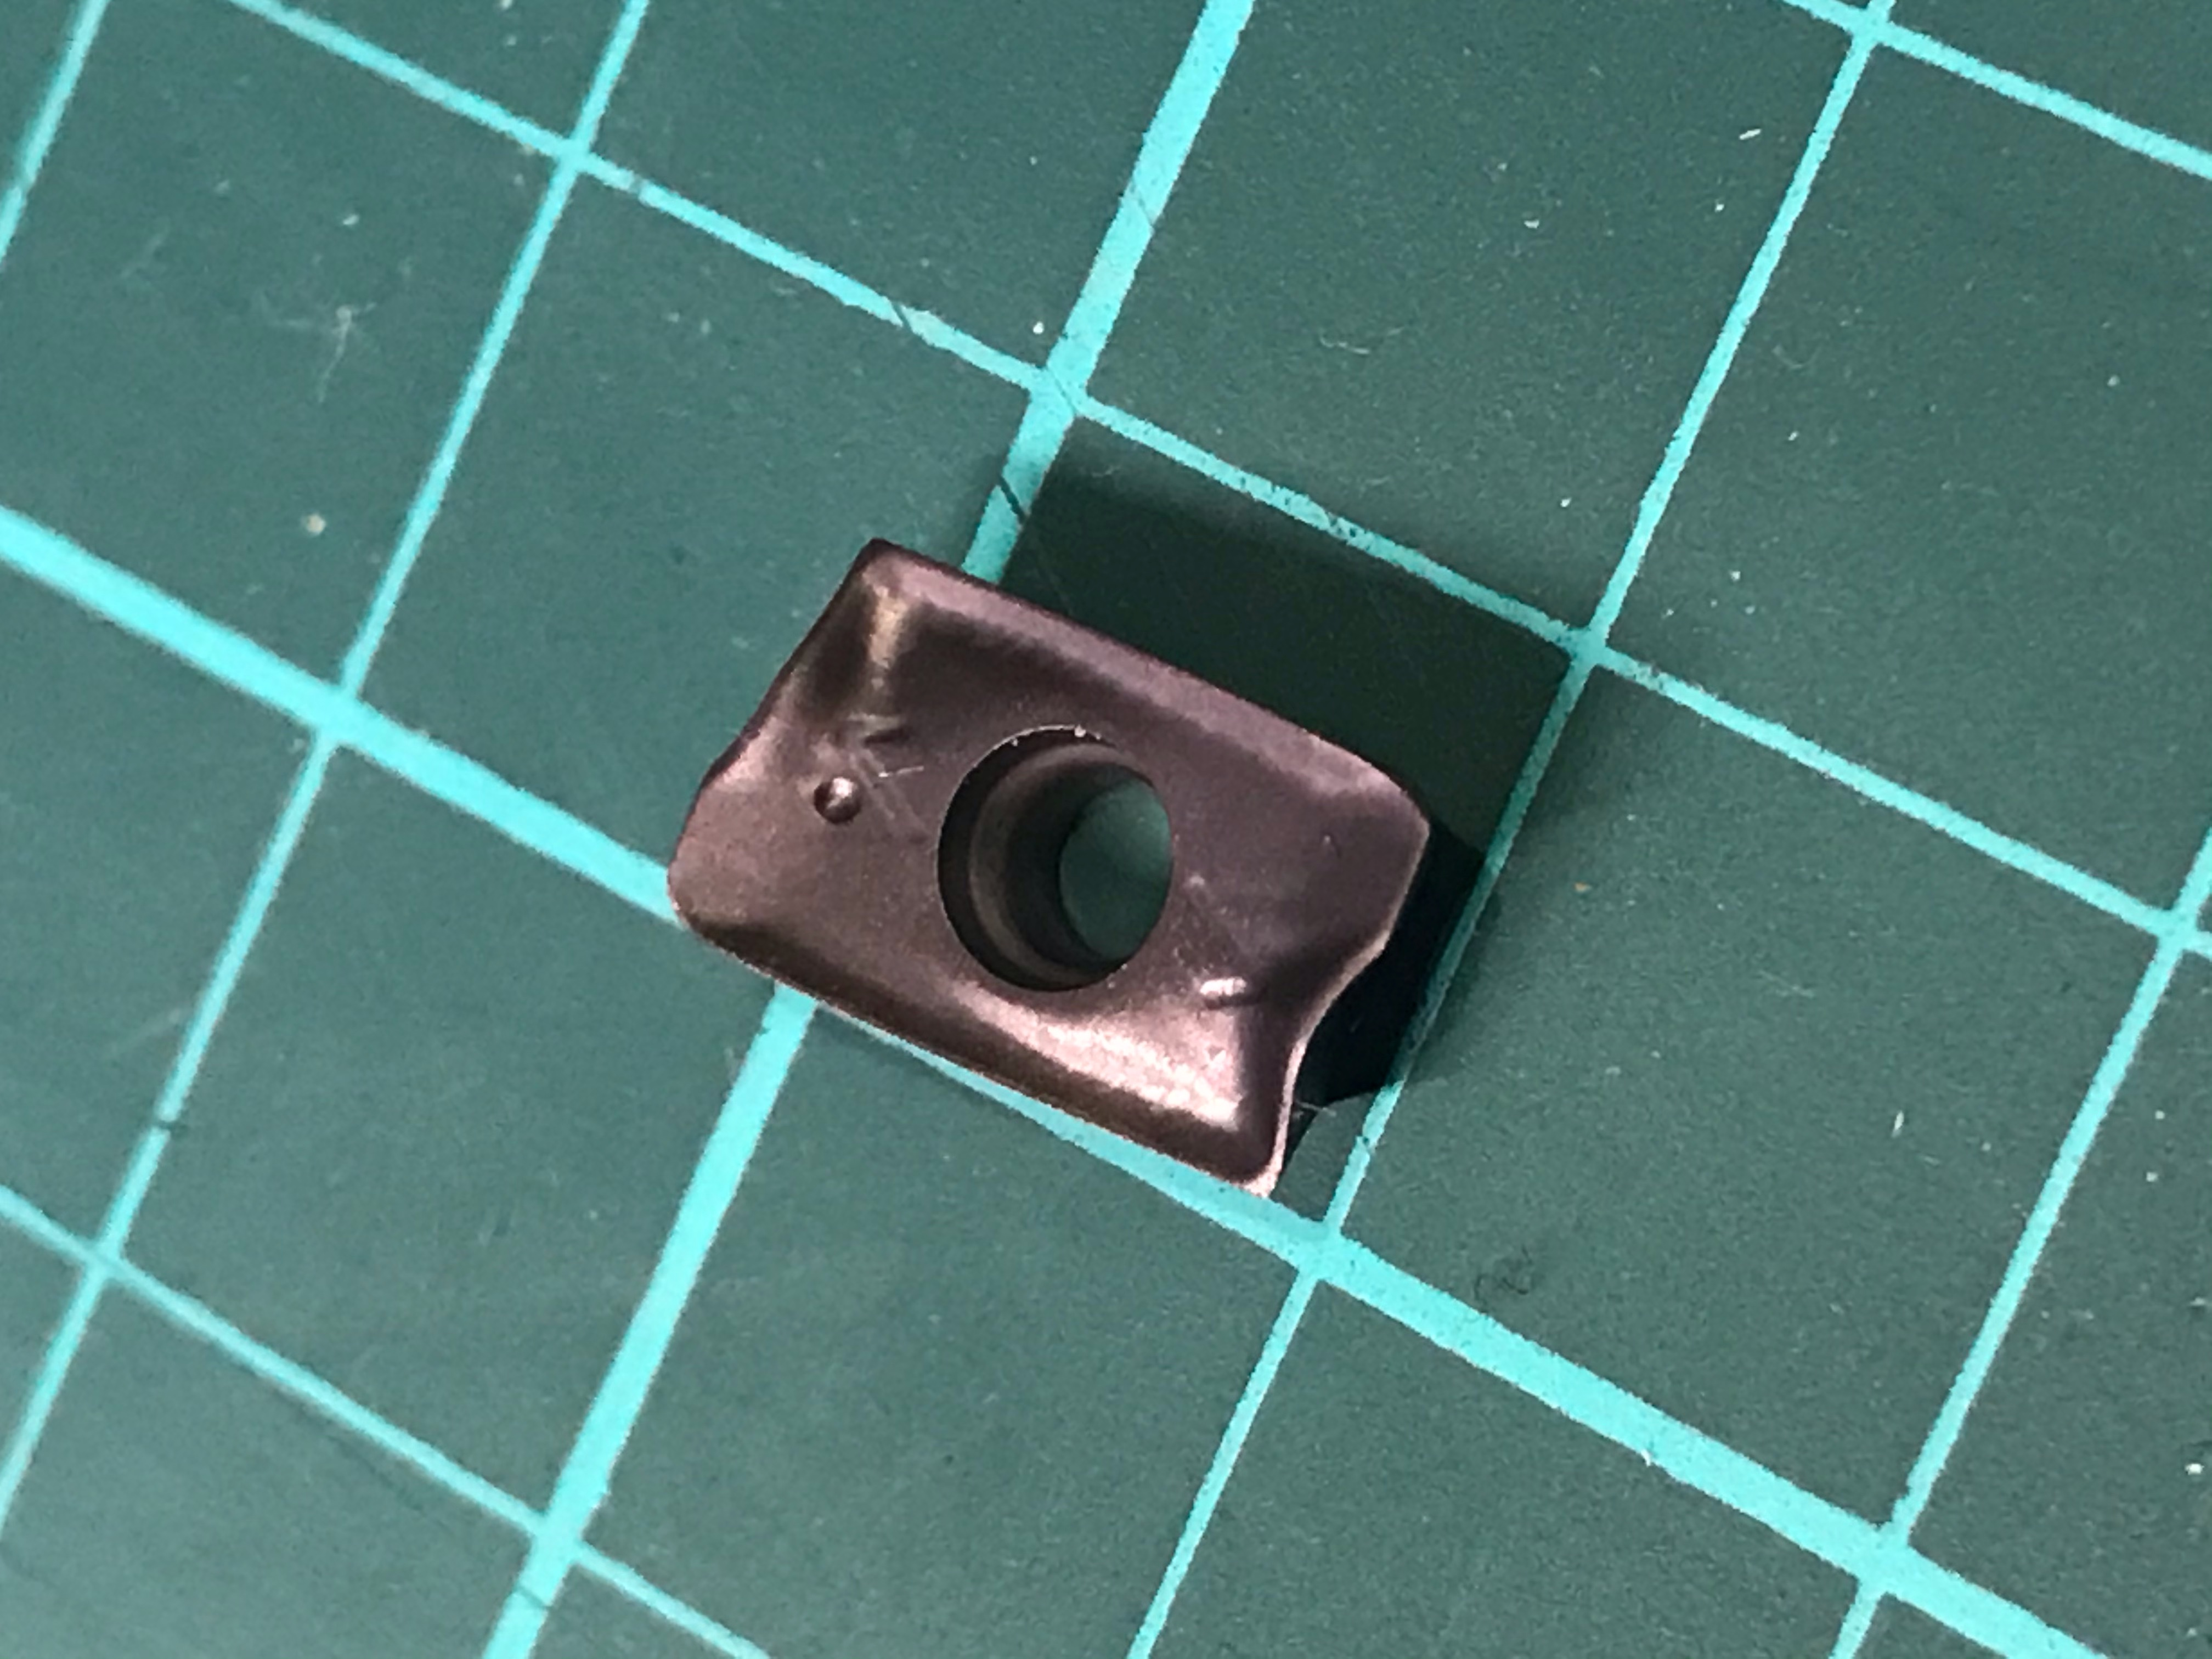
\includegraphics[width=4.166667in, keepaspectratio=true]{./ZimFiles_files/Verslagen/Activiteiten_rapport/Activities/Masterproef_Tool_Wear_Inspection_-_Update_4_TG/plaatje_1cm.jpeg}



Ik heb al een aantal beelden kunnen maken (in bijlage te vinden), maar er is nog wat finetuning nodig om de camera positie en hoek beter te kunnen regelen om ook de invloed daarvan te kunnen meten.

De komende weken zal ik deze opstelling nog afwerken en zoeken naar een ideale camera hoek door wat beelden door een simpel netwerk laten gaan en de resultaten te vergelijken voor verschillende camera posities waarbij de licht condities niet wijzigen.

 

Met vriendelijke groeten,

 

Lars De Pauw



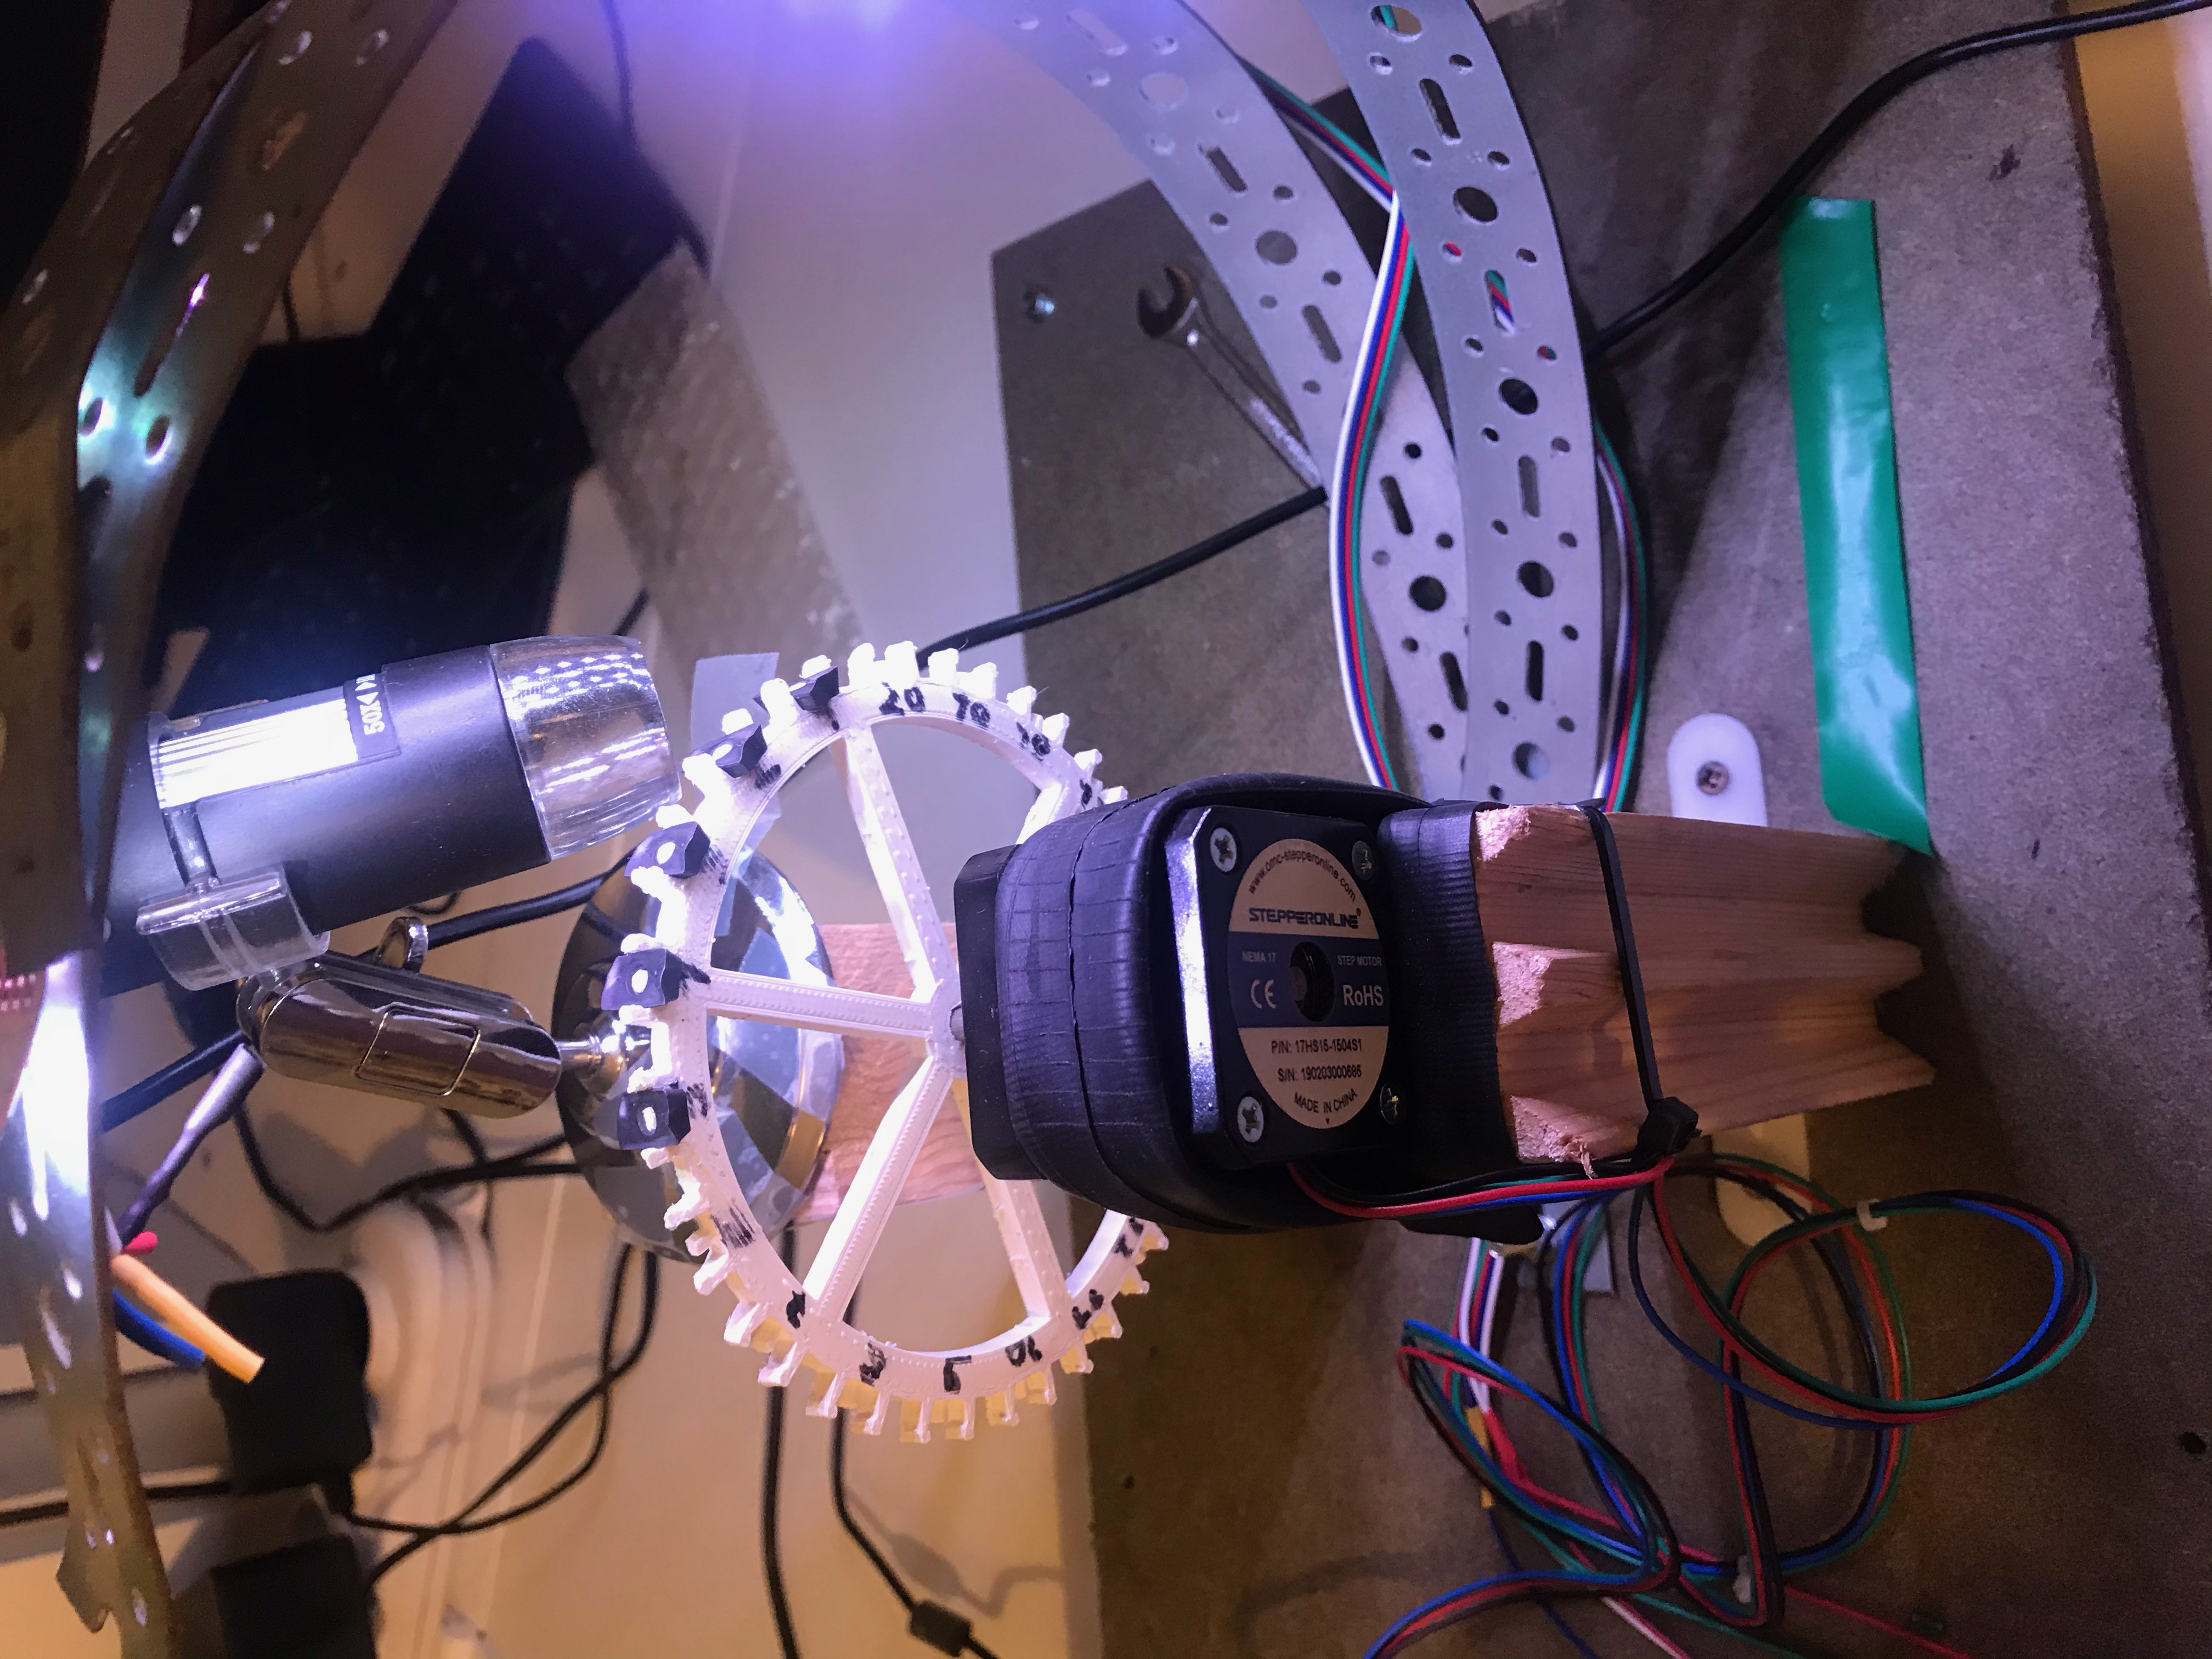
\includegraphics[width=4.166667in, keepaspectratio=true]{./ZimFiles_files/Verslagen/Activiteiten_rapport/Activities/Masterproef_Tool_Wear_Inspection_-_Update_4_TG/rechts_licht.jpeg}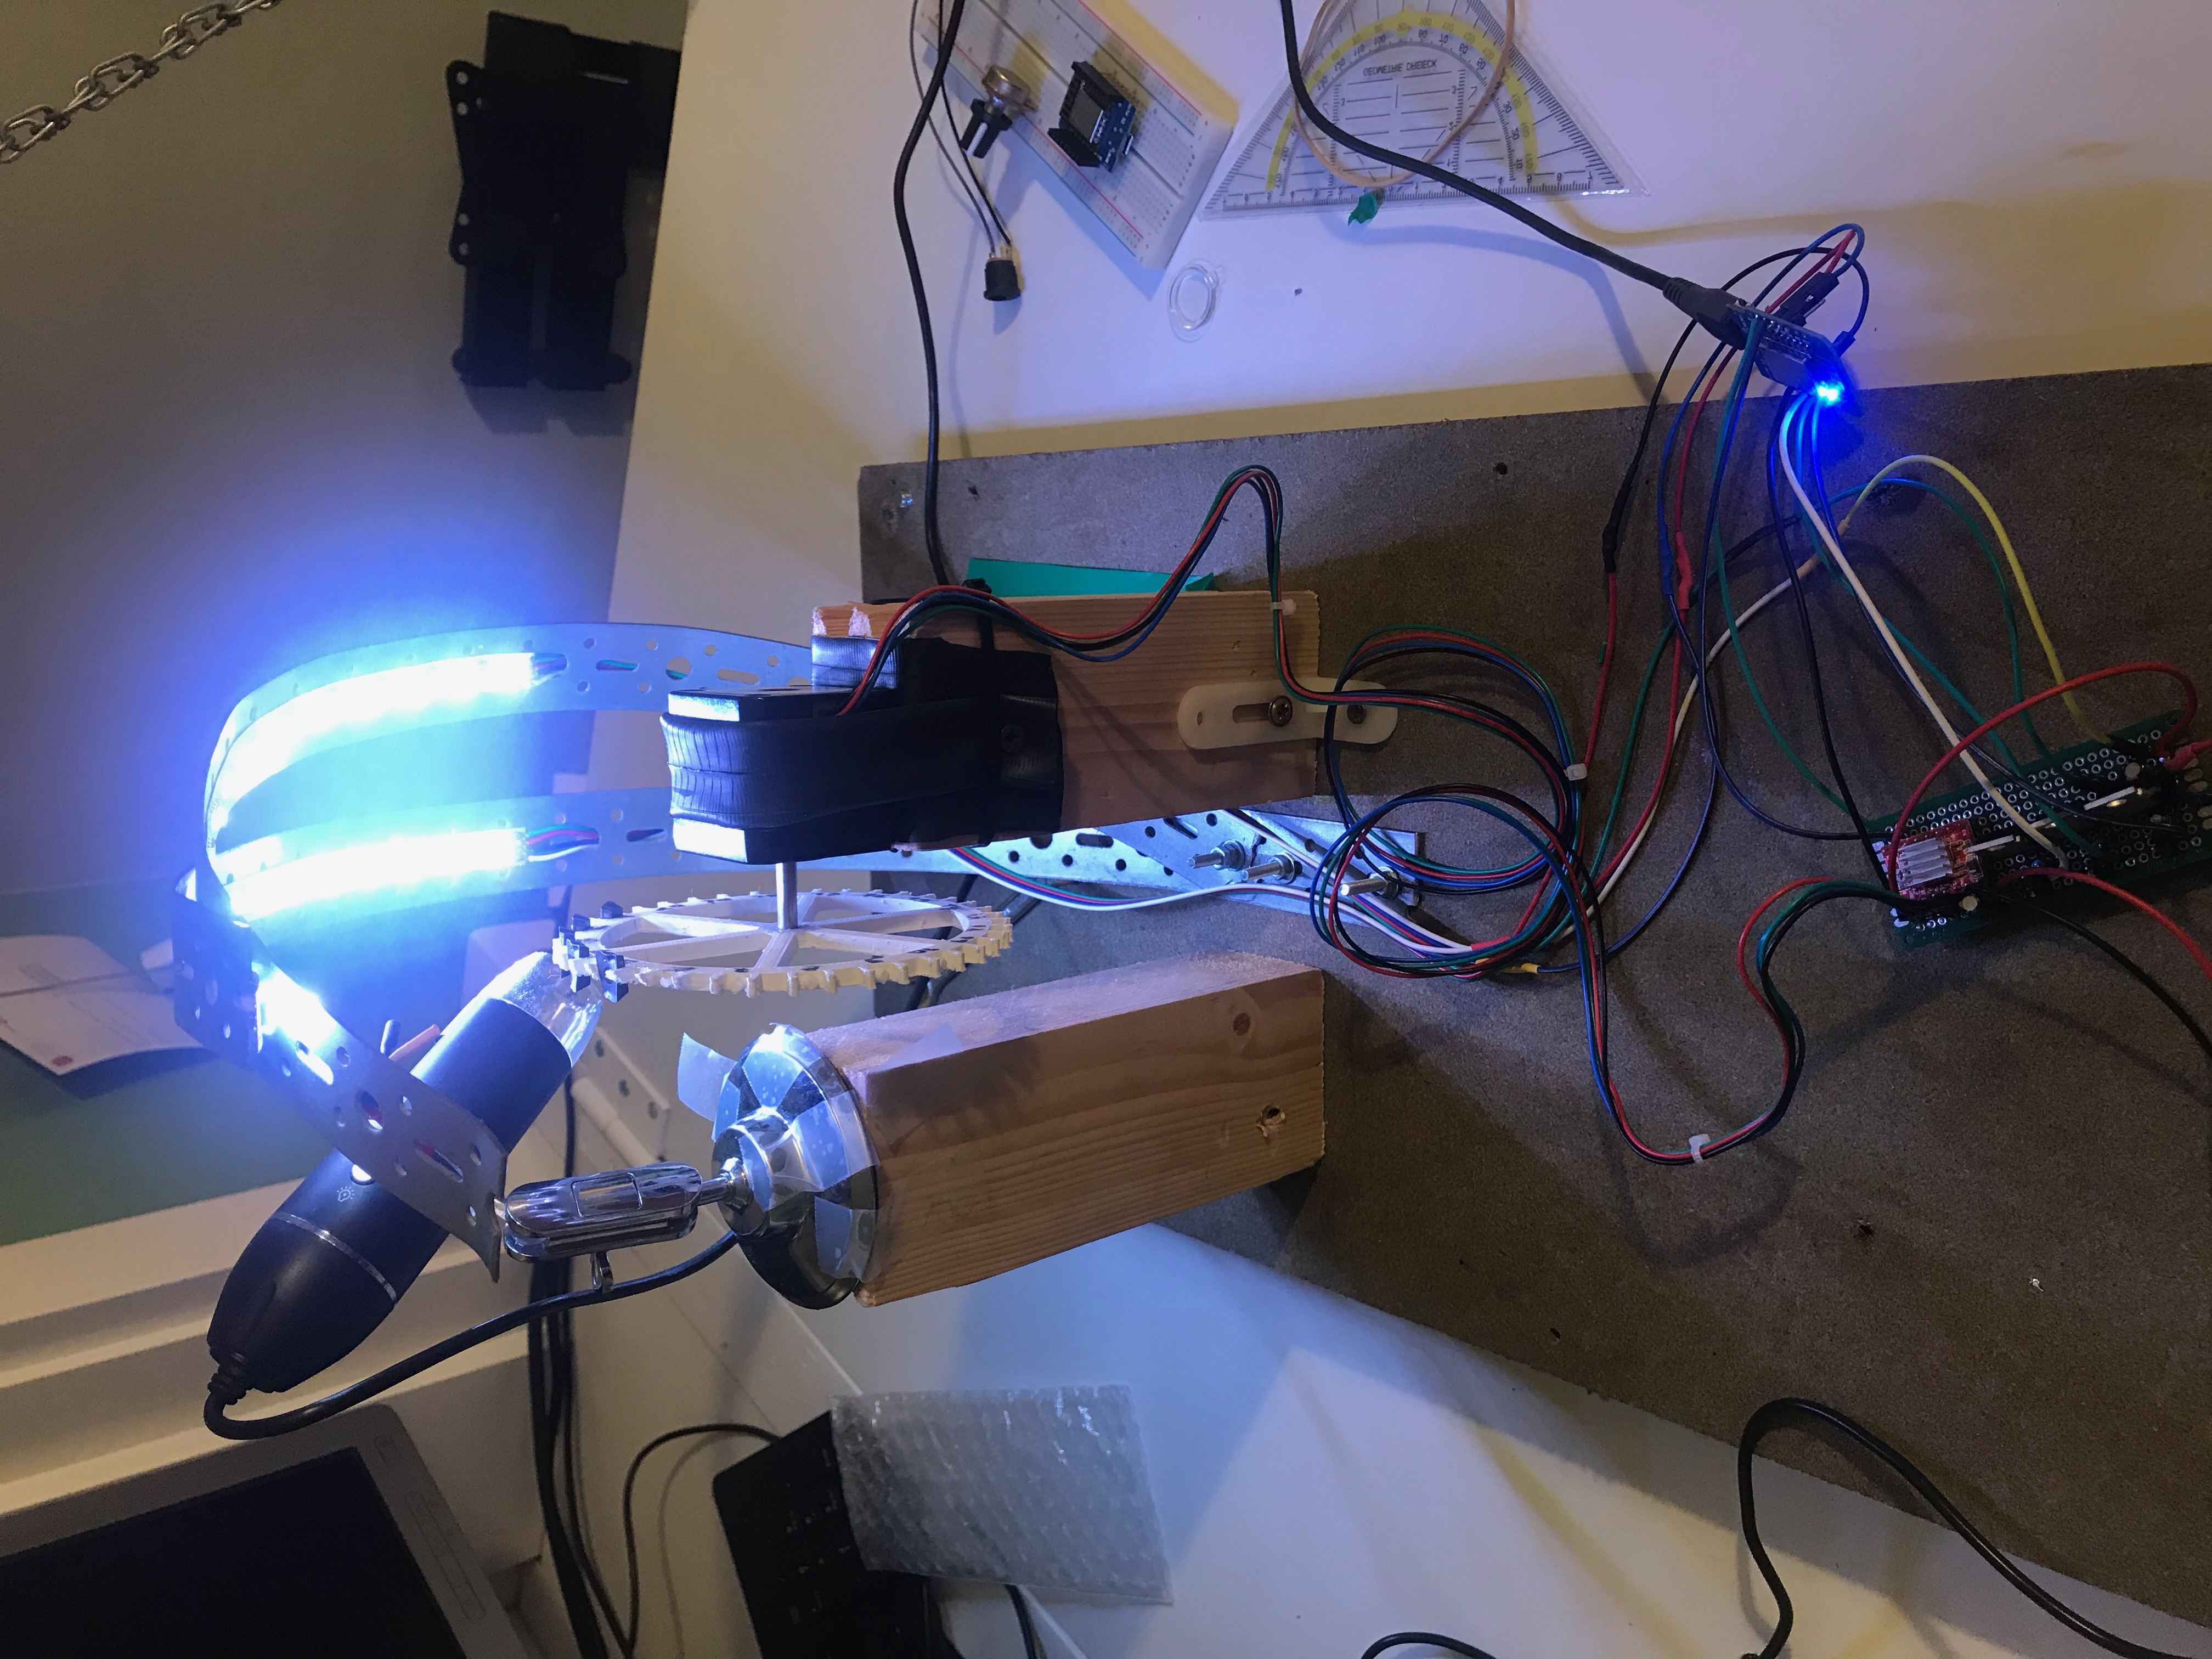
\includegraphics[width=4.166667in, keepaspectratio=true]{./ZimFiles_files/Verslagen/Activiteiten_rapport/Activities/Masterproef_Tool_Wear_Inspection_-_Update_4_TG/achter_licht.jpeg}



\includegraphics[width=4.166667in, keepaspectratio=true]{./ZimFiles_files/Verslagen/Activiteiten_rapport/Activities/Masterproef_Tool_Wear_Inspection_-_Update_4_TG/p4_l9.png}\includegraphics[width=4.166667in, keepaspectratio=true]{./ZimFiles_files/Verslagen/Activiteiten_rapport/Activities/Masterproef_Tool_Wear_Inspection_-_Update_4_TG/p4.png}


		\section{Masterproef Tool Wear Inspection - Update 5 DH}

Created woensdag 25 november 2020



Meeting 25/11/2020

Dries Hulens



Te bespreken:



Wat is al gedaan?

\begin{itemize}
\item Setup bijna klaar, geen gebruik maken van de lange ledtrips, enkel de adresseerbare leds. 
\item Enkele tests met het maken van foto’s
\item Model aangemaakt Resnet18 met transfer learning om de setup mee te testen.
	\begin{itemize}
	\item Is het hier belangrijk dat er een hoog percentage gehaald wordt? 
	\item Eventueel met 60 plaatjes ook mogelijk?
	\item 3 wielen geprint waarop plaatjes geklikt kunnen worden zodat ze kunnen blijven zitten terwijl andere worden gefotografeerd.
	\item Beperkt documenteren van de keuze van de architecturen
	\item Beperkt documenteren van licht reflecties
	\end{itemize}
\end{itemize}


Wat nog gedaan moet worden dit semester:

	\begin{itemize}
	\item Heel veel schrijven aan tussentijds verslag
		\begin{itemize}
		\item Valt wel mee, goed documenteren
		\end{itemize}
	\item Setup vervolledigen met camera standaard en eventueel extra ledstrip
		\begin{itemize}
		\item Gewoon de setup nog maken en een dataset aanleggen, die dataset eens door het huidige model laten gaan mits gegevens van Tom Jacobs er zijn.
		\end{itemize}
	\item Zelf eerst foto’s filteren.
		\begin{itemize}
		\item Kijken waar een grote blob lichte pixels te zien is, die foto’s door het model laten gaan en de andere niet?
			\begin{itemize}
			\item Misschien beter dat netwerk beslist, een foto kan goed lijken voor een mens, maar het netwerk kan op andere dingen letten.
			\end{itemize}
		\end{itemize}
	\item Grotere dataset aanmaken met alle tot nu toe beschikbare plaatjes
	\end{itemize}




Vragen

	\begin{itemize}
	\item 3D printen pet PETG? 
		\begin{itemize}
		\item T hoger
		\item Bed 80°
		\item Plooibaar bed nemen
		\end{itemize}
	\item Goed als ik slechts een paar modellen implementeer en geen diepgaand onderzoek doe?
		\begin{itemize}
		\item Standaard notebook nemen waarin de verschillende naast elkaar worden getest. 
		\item Zien met suggestie van Floris De Feyter: Weights and biases -\textgreater{} is voor model optimalisatie, hoeft hier niet meteen, moet gewoon zien of iets beter is of niet
		\end{itemize}
	\item Richtlijn voor aantal pagina’s voor de related work sectie
		\begin{itemize}
		\item Afhankelijk
		\end{itemize}
	\end{itemize}


	\begin{itemize}
	\item Richtlijnen voor de gehele paper, dingen die moeten worden besproken met promotor:
		\begin{itemize}
		\item Mag we gebruikt worden in het onderzoek, aan te raden of niet?
		\item We mag zeker
		\end{itemize}
	\item Mogen de bronnen in Harvard systeem weergegeven worden?
		\begin{itemize}
		\item Harvard systeem hanteren
		\end{itemize}
	\item Wanneer moet de masterproef tekst nagelezen worden? 1 week op voorhand?
		\begin{itemize}
		\item 1 week zeker goed
		\end{itemize}
	\item Pytorch lightning?
		\begin{itemize}
		\item Mr Ophoff of de feyter eens vragen, zij gebruiken het regelmatig.
		\end{itemize}
	\end{itemize}


Cross validation

	\uline{Opzoeken} 
	
	Kan setting zijn bij dataloaders
	
	



Presentatie al eens op voorhand doorsturen naar promotor om na te laten kijken



Diepte van netwerken onderzoeken:

	Wat geeft een dieper netwerk op de verschillende aantallen foto's
	
	Darknet
	
	Resnet 
	


Beste netwerk plotten van verschillende architecturen

	om een weergave te hebben van welke netwerken het beste waren. 
	
	




		\section{Done}

Created vrijdag 20 november 2020



\subsection{Wat is er reeds gedaan deze periode tot 10 November?}



\subsection{Week 05/10/2020 - 11/10/2020}

opstellen en indienen van het tussentijds verslag in de eerste helft van de week.

Na 07/10/2020 was het verslag ingediend en werd gestart met het formuleren van een beschrijving van het probleem.

Het schrijven ging zeer moeizaam omdat ik weinig perspectief had over wat het doel van de masterproef was. Het is ook zeer moeilijk om een weg te banen tussen alle literatuur en de goede er tussenuit te vinden. Er werd heel wat tijd verspild met het lezen van bronnen die onvoldoende zijn of net niet goed genoeg waren. Hier moest een systeem in gevonden worden om de bronnen snel te kunnen inschatten. 



\begin{enumerate}[1]
\item bezoek gebracht aan Tom Jacobs van Sirris om de eerste plaatjes op te halen. 
	\begin{itemize}
	\item frees getoond en 
	\item uitleg gegeven over het bredere kader van het onderzoek. 
	\item Een verslag is hier te vinden. 
	\end{itemize}
\item Bedrijfs bezoek bij Aperam waar een vriend een visie inspectie systeem heeft geïnstalleerd dat fouten detecteerd in grote stalen platen. 
	\begin{itemize}
	\item Hier was het zeer nuttig om eens te zien hoe een systeem wordt geïmplementeerd in een productielijn. 
	\item De schaal was hier wel een stuk verschillend waardoor er niet echt dingen kunnen overgenomen worden.
	\end{itemize}
\item Start aan een beschrijving van het verleden van dit onderwerp.
	\begin{itemize}
	\item ging zeer moeizaam om dezelfde redenen als het zoeken van de probleem beschrijving.
	\end{itemize}
\item Implementatie maken voor een binair transfer learning model dat bepaald of een tool versleten is of niet. te vinden in \href{https://colab.research.google.com/drive/1N2r6nplmx88pUOKkLN0Hmy42D7YRUypC}{TWI 5} Dit bouwde verder op \href{https://colab.research.google.com/drive/1Qsoj7WmGClsslivGGI4DGL10NNVdIHC2}{TWI 4} waar een zelfde model werd gemaakt zonder tranfer learning.  \href{https://colab.research.google.com/drive/1Qsoj7WmGClsslivGGI4DGL10NNVdIHC2}{TWI 4} is een volledig werkend prototype van een algoritme in Keras.
\item implementatie maken voor een classificatie model \href{https://colab.research.google.com/drive/1QN68qaE84fq9dBnZFNExsS5F8tZk-8Ow}{TWI 6} in Keras waarbij tranfer learning wordt gebruikt. Hierbij waren alle voorspellingen voor dezelfde klasse. Niet verklaard hoe dit kon, misschien omdat de data niet gelijk verdeeld was over de klassen. De beste learning rates waren reeds bepaald voor dit probleem en lagen rond 3e-5 
\end{enumerate}


Voor alle bovenstaande tests werden de labels van labels3.csv gebruikt op de first handmade dataset





\subsection{Week 12/10/2020 - 18/10/2020}



\begin{enumerate}[1]
\item Verder schrijven aan het verleden van het onderwerp. 
	\begin{enumerate}[a]
	\item Ging zeer moeizaam en vergde veel tijd voor zeer weinig resultaat. 
	\item Gekomen tot een aantal bronnen. 
	\item opzetten mendeley om bronnen in bij te kunnen houden.
	\end{enumerate}
\item Aanmaken van Engelse latex file op overleaf
\item implementatie maken in keras waarbij een regressie model wordt getraind op de eerste honderd foto's die verkregen zijn
	\begin{enumerate}[a]
	\item fotos te vinden als first handmade dataset
	\item Een regressie model wordt niet ondersteund door Keras waardoor het zeer omslachtig was om de labels en de foto's met elkaar te kunnen verbinden. Dit zorgde voor heel wat problemen.
		\begin{enumerate}[1]
		\item classificatie model met transfer learning maken met Keras dat de gegevens opdeeld in 3 klassen waarbij ook een verschillende batch size werd getest. Te zien in \href{https://colab.research.google.com/drive/1QN68qaE84fq9dBnZFNExsS5F8tZk-8Ow}{TWI 6} en  \href{https://colab.research.google.com/drive/1zeKin3shLk_ogrFCwHrzpnjJmaWaoCq0#scrollTo=CDnGBD0NGkbM}{TWI 7}
		\item proberen de labels toch gelinkt te krijgen via de data loader functies van Keras. Dit werkte echter niet dus werd een andere methode geprobeerd
		\item Het regressie probleem omzetten in een classificatie model wat betreft de data. Hiervoor werd een map aangemaakt per waarde en dus per foto om zo de gegevens in te lezen. Dan werd de model architectuur aangepast zodat deze een output gaf van een getal waarde in dezelfde grootte orde als de waarden van de metingen. 
		\end{enumerate}
	\end{enumerate}
\end{enumerate}
			Dit werkte echter ook niet en er werden geen resultaten bekomen.
			
			De uitwerking is te vinden op Google Colab onder de naam \href{https://colab.research.google.com/drive/1qR4reWAIvIs59eZKWSmZHboZ1gjGA4jS}{TWI 8} waarbij ook transfer learning werd toegepast om de weinige data toch te kunnen omzetten in een werkend model
			
\begin{enumerate}[1]
\setcounter{enumi}{3}
\item Er werd gekeken welke andere frameworks er nog zijn en wat het verschil is tussen deze. Hier is ook beslist om verder te gaan met Pytorch gezien dit het meest open framework is. 
\end{enumerate}


\subsection{Week 19/10/2020 - 25/10/2020}



\begin{enumerate}[1]
\item Een nieuwe implementatie \href{https://colab.research.google.com/drive/1f-Rfei8QrHotvgktp8hzviR8dv1XJJjz}{TWI 9} waarin een eerste model werd gemaakt met pytorch. 
	\begin{enumerate}[a]
	\item er werden wat problemen gevonden bij het tonen van de foto's eens ze genormaliseerd waren waardoor het moeilijk was om de data voor te stellen die gebruikt werd. 
	\item Een model van het internet werd geïmplementeerd en er werden resultaten bekomen ± 60\% accuracy op de train en validation data. Dat lijkt niet zo correct. op een test set van slechts enkele beelden werd 25\% accuracy gehaald. Er leek ergens iets mis te zijn met de transformaties van de foto's naar pil voorstelling. 
	\end{enumerate}
\item Een binaire classificatie implementatie \href{https://colab.research.google.com/drive/1t4Yvzj1rqNy24pj4dDtyBH2CStDePXMw}{TWI 10} werd gemaakt waarin een zelfde model architectuur werd geprobeerd te maken als bij het model van Keras. 
	\begin{enumerate}[a]
	\item Echter was dit zeer lastig zonder voorkennis van hoe architecturen er uit zien. Door het sterk verschil in benamingen tussen functies is dit niet geslaagd. 
	\item De foto's in juiste mappen plaatsen via een programma werd ook gerealiseerd na heel wat problemen met de google colab mappen structuur. 
	\item In het model waren de data augmentation regels te hard. Hierdoor werden de foto's zeer sterk bewerkt wat zorgde voor heel wat meer foto's, maar tegelijk deed het afbreuk aan het model gezien de foto's in het echt makkelijker te interpreteren vallen. 
	\item De training en validation loss ging niet naar beneden tijdens de training.
	\end{enumerate}
\item Meeting met Dries Hulens waarin werd overlopen hoe de opstelling zou gemaakt worden en waar op te letten.
	\begin{enumerate}[a]
	\item hierbij werd aangehaald dat het schrijven nog niet belangrijk zou zijn, en dat dit nog even kon wachten tot december eventueel.
	\item licht reflecties onderzoeken hoe het materiaal reageerd op bepaalde licht frequenties.
	\item eventueel kijken of een stuk uit de fotos kan gesneden worden (felste blob) om enkel daar het model mee te voeden.
	\item adresseerbare ledstrip mee gekregen
	\item camera mee gekregen.
	\end{enumerate}
\item Een eerste testopstelling maken om de camera te leren gebruiken.
	\begin{enumerate}[a]
	\item De camera moest zeer goed ingesteld worden om een scherp beeld te krijgen van de slijtage
	\item Setup is besproken in: first camera mount
		\begin{enumerate}[1]
		\item hiervoor is een houder ge 3D print.
		\item De belichting besproken in desk lamp test
		\item de camera werd met de normale houder op de bureau gezet. 
		\end{enumerate}
	\item De beelden hiervan waren zeer indrukwekkend en gaven een mooi resultaat zonder veel werk te hoeven steken in een setup.
	\end{enumerate}
\end{enumerate}


\subsection{Week 26/10/2020 - 1/11/2020}



\begin{enumerate}[1]
\item 3D model gemaakt van het eerste rad dat gebruikt zal worden voor een automatisch systeem dat de plaatjes voor de camera beweegt.
	\begin{enumerate}[a]
	\item Creatie van een 3D model
	\item 3D printen 
	\item berekening welke nauwkeurigheid nodig is om de stappen motor aan te sturen
	\end{enumerate}
\item Een programma aangemaakt om de stepper motor aan te sturen met de motor drivers. 
\item documenteren van de afgelopen tests
\item Test met vaste led strips om ze te kunnen aansturen vanaf een raspberry pi
	\begin{enumerate}[a]
	\item Ging niet goed met zeer kleine transistors. 
	\item overgeschakeld naar relais. Gaf zeer veel problemen met solid state relais die ook in gesloten toestand nog een stroom doorlieten.
	\item Gewone analoge stuurbare relais werkten wel, maar maken een klik geluid. 
	\item Volgende stap is om mosfets te gebruiken voor deze sturing.
	\item Test met verschillende voltages met een potentiometer voor de strips.
	\end{enumerate}
\item PCB maken om de aansturing mogelijk te maken gezien het breadboard de hoge stroom niet aan kan. 
\end{enumerate}


\subsection{Week 02/11/2020 - 08/11/2020}



\begin{enumerate}[1]
\item Ophalen van een volgende batch plaatjes
	\begin{enumerate}[a]
	\item bekijken hoe de plaatjes worden gelabeld. 
	\item opzoeken en documenteren of de plaatjes reageren op een bepaalde golflengte zonder goede resultaten, dit moet nog verder onderzocht worden.
	\item materialen van de plaatjes opzoeken
	\item Afslijting komt recht op de hoek van het plaatje
	\item Frees kan niet zelf nauwkeurig draaien, een mogelijke oplossing is de voledige snijplaat houder uit de frees halen en fotograferen.
	\item Er zijn ongeveer 4 hoofdklassen van slijtages, maar deze zijn moeilijk zelf na te maken
	\item Een extra metric toevoegen die de oppervlakte van de slijtage weergeeft. 
	\end{enumerate}
\item Een testopstelling gemaakt met het rad met de stepper motor en enkele bandijzers om de leds aan te bevestigen.
\item Arduino finetunen zodat deze volledig werkt met de adressable led en de motor makkelijk kan aangestuurd worden met commandos via de seriele input.
\item Eerste beelden maken met een geautomatiseerde setup
	\begin{enumerate}[a]
	\item zie first automated dataset
	\item werkte niet, de communicatie tussen de computer en arduino was te traag. Dit wordt (tijdelijk) opgelost door delays te plaatsen die de trage communicatie opvangen. 
	\item Eerste beelden konden gemaakt worden en het python script is gemaakt.
	\end{enumerate}
\item PCB finetunen 
	\begin{enumerate}[a]
	\item nieuwe weerstand die de spanning begrensd voor de ledstrip
		\begin{enumerate}[1]
		\item is doorgebrand en terug vervangen door een grotere weerstand
		\end{enumerate}
	\end{enumerate}
\end{enumerate}


\subsection{Week 09/11/2020 - 15/11/2020}

\begin{enumerate}[1]
\item Oplossen van het probleem van de trage communicatie tussen de computer en arduino. 
	\begin{enumerate}[a]
	\item Dit lag aan een time delay die gezet was voor het inlezen van een nieuwe lijn van de seriele input. 
		\begin{enumerate}[1]
		\item door de tijd te verlagen van de delay was het probleem al grotendeels verholpen. (van 1 seconde naar 10 miliseconden)
		\item Door een nieuw line end karakter te kiezen was het probleem volledig weg. Dit stond op '$\backslash$0', wijzigen naar / was voldoende om het einde van de lijn aan te geven
		\end{enumerate}
	\end{enumerate}
\item Nieuwe foto's nemen met de aangepaste code. Te zien in second dataset
\item Een nieuw rad ontwerpen dat toelaat om de plaatjes makkelijker te monteren en demonteren door clips te gebruiken waardoor de plaatjes niet met hun snijkant moeten glijden over plastiek. Dit zorgt er ook voor dat de clips makkelijk kunnen aangepast worden om met toekomstige veranderingen mee te kunnen.
	\begin{enumerate}[a]
	\item Het 3D model van de plaatjes online gevonden waardoor de juiste afmetingen bekend waren.
	\item Het 3D model printen zorgde er voor dat de afmetingen van de modellen niet werden gerespecteerd. Hierdoor pasten de eerste tests niet. Door Steeds 0.4 mm extra te rekenen voor elke maat paste het wel. 
	\item De clips werden geprint met een langere midelste pin om deze makkelijk van het rad te kunnen verwijderen. 
	\end{enumerate}
\item Bijwonen van de presentaties van twee studenten die in januari hun masterproef zullen indienen om een beeld te krijgen van hoe de presentaties in elkaar zitten.
\item Alle bestanden die tot hiertoe gemaakt zijn reorganiseren en opslaan in GITHUB.
	\begin{enumerate}[a]
	\item werken met meerdere branches. 
	\item Master branch 
	\item develop branch
	\item feature/\textless{}featurename\textgreater{} branch
	\end{enumerate}
\item Belichten van de fotos verliep zeer goed, alleen was het zeer moeilijk om de camera te positioneren en scherp te stellen met de huidige standaard. Hiervoor werd gevraagd of nieuwe materialen konden besteld worden om deze standaard te vervangen.
\item Vraag om ander print materiaal te kunnen gebruiken voor de print van de clips. Nu werd witte PLA gebruikt wat nogal snel afbreekt, met PETG hopen we de problemen niet meer te hebben.
\item Aanmaken van een nieuwe dataset met de eerste batch van plaatjes gezien niet duidelijk was welke kant de a kant was en welke de b-kant.
	\begin{enumerate}[a]
	\item Dit werd gedaan met een simpele setup waarbij de camera op de bureau stond en handmatig werden van alle plaatjes foto's genomen en vergeleken met de gekregen foto's van Sirris.
	\item Blijkt dat de B kant de kant is met de streep
	\end{enumerate}
\end{enumerate}


\subsection{Week 16/11/2020 - 22/11/2020}



\begin{enumerate}[1]
\item verder bouwen op de netwerken die reeds gemaakt waren om een model te verkrijgen dat de camera setups zal kunnen beoordelen met zo min mogelijk afbeeldingen. netwerk wordt getraind met de beelden van de tweede hand made dataset
	\begin{enumerate}[a]
	\item dit werkte niet zo goed. daarom terug van nul begonnen met het opbouwen van de modellen. 
	\item Duurde zeer lang om de foto's juist ingelezen te krijgen.
	\item Een klassificatie netwerk kunnen opbouwen met transfer learning met een Resnet18 architectuur
	\item \href{https://colab.research.google.com/drive/1iUkA7DjNarxSnYvV8T397PHwNeK0OGI1}{TSU\_Resnet18\_1} proberen van een tutorial een model op te bouwen from scratch, heeft niet gewerkt doordat er te veel aanpassignen waren die niet nodig waren. bijvoorbeeld zelf een dataset klasse aanmaken
	\item \href{https://colab.research.google.com/drive/1uh-lWXxS50Y3o4Fly4Wq9ZXmDzeXVAKN}{TSU\_Resnet18\_2} is een bestand waarin het veel makkelijker wordt gedaan en waar de code werkt. Komt uit op een test accuracy van 88\% Dit zal nog hoger moeten worden met betere foto's, maar is een zeer goed begin met slechts 100 foto's
	\item Het tweede gevonden netwerk is incept
	\end{enumerate}
\item Onderzoeken welke netwerk architecturen goed zijn voor projecten met zeer weinig data
	\begin{enumerate}[a]
	\item alles met weinig parameters is makkelijk te trainen. 
	\item steeds met transfer learning werken om goede resultaten te bekomen
	\item 20 beelden om een setup te beoordelen zal te weinig zijn. eventueel meerdere wielen printen om alle plaatjes op een wiel te kunnen monteren om zo zeer snel alle plaatjes te kunnen fotograferen met steeds een verschillende camera positie
	\end{enumerate}
\item Masterproef opgave lezen om te weten wat de literatuur studie/ tussentijds verslag inhoud.
	\begin{enumerate}[a]
	\item Tegengekomen dat een activiteiten verslag moet ingediend worden 
	\end{enumerate}
\item activiteiten verslag aanmaken waarin alles wordt besproken wat per week gebeurt is en wat er te doen is voor de komende weken.
\end{enumerate}


\subsection{Week 23/11/2020 - 29/11/2020}

Dinsdag 24/11/2020

\begin{enumerate}[1]
\item Verschillende architecturen testen met en zonder transfer learning
\item opzoeken over Weights and biases en implementeren
\end{enumerate}


Woensdag 25/11/2020

\begin{enumerate}[1]
\item \href{https://wandb.ai/dplars/pytorch-twi_second_handmade_sweep?workspace=user-dplars}{Weights and biases sweep} implementeren en eerste 500 sweeps uitvoeren, tijdens de nacht nog 2500 laten uitvoeren.
\item Afwerken van de camera setup, verschillende dingen 3D printen om camera te kunnen monteren. Veel moeite met de PETG degelijk te laten printen, na veel werk lukte het. Het probleem was dat de PETG niet genoeg plakte aan het bed met de toen ingestelde settings. Uiteindelijk geprint met 240 nozzle temperatuur en 60 bed temperatuur met steeds een ondervlak onder de print zodat deze zeker niet zou bewegen.
\item Meeting met Dries Hulens, bespreken wat er dit semester nog zal gebeuren en hoe het tussentijds verslag en de presentatie er uit zien. 
\end{enumerate}


\subsection{Week 30/11/2020 - 06/12/2020}

Maandag, dinsdag

3D printen van de nodige wielen en clips. Met zeer veel problemen met 3D printer waarbij printer ook stuk is gegaan, terug gerepareerd en verder gewerkt. Alle tandwielen uiteindelijk woensdag geprint gekregen. 

Meeste plaatjes op de wielen gestoken en die van het eerste wiel voor batch 1 en 2 omgedraaid zodat deze ook met de 'bullet' naar dezelfde kant wijzen als de ander wielen. Echter zit hier nog een probleem dat deze rechtsdraaiend genummerd zijn in plaats van linksdraaiend zoals op de andere wielen. Dit moet nog opgelost worden of ze moeten nog op een zwart wiel.



Woensdag

Overige clips en rad geprint en plaatjes op de raden gestoken. 

Een deel gedocumenteerd over de aangelegde datasets:

\begin{itemize}
\item Vision:Dataset:automated datasets:1 check camera position:1 camera position side aangevuld
\item Vision:Dataset:automated datasets:1 check camera position:2 camera position top aangevuld
\item Vision:Dataset aangevuld
\end{itemize}




Afwerken van de setup door toevoeging van nieuwe staander voor motor

aanmaken van een nieuwe dataset genaamd spaghetti met vier foto's per plaatje



foto's van spaghetti door algoritme laten gaan en sweep laten uitvoeren. Eerste resultaten zien er zeer slecht uit. Slechtere accuracy dan bij de vorige dataset die met de hand was gemaakt. (second handmade dataset)

Wel meer data om te testen en valideren. Test resultaten zien er wel beter uit.



wandb proberen instellen om te runnen vanaf mijn eigen computer tot hiertoe zonder succes



Vrijdag

Documenteren van de verschillende tests die uitgevoerd werden op de verkregen datasets.

zie:

\begin{itemize}
\item All networks 1
\item All networks 2
\item All networks 4 Spaghetti
\item All networks 4 Spaghetti first 5 batches
\end{itemize}


Aanmaken pagina met foto's van nieuw rad v2



Datasets documenteren:

Spaghetti dataset


		\section{ToDo}

Created vrijdag 20 november 2020



\subsection{Week 09/11/2020 - 15/11/2020}



\subsubsection{short term}

\begin{enumerate}[1]
\item netwerk maken om camera setup mee te beoordelen
\end{enumerate}


\subsubsection{Long term}

\begin{enumerate}[1]
\item Tekst schrijven
\end{enumerate}


\subsection{Week 16/11/2020 - 22/11/2020}



\subsubsection{short term}

\begin{enumerate}[1]
\item inception v3 implementeren, nieuwe foto's door het netwerk laten gaan
\item foto's nemen onder verschillende camera hoeken
\item nieuw rad printen 
\item extra clips printen in PETG
\item nieuwe camera standaard maken waarop posities te veranderen zijn.
\item Extra ledstrip toevoegen aan setup
\item Documenteren over PCB
\item Documenteren over netwerken in vloeiende tekst
\item Labels verkrijgen van extra plaatjes bij Tom Jacobs
\end{enumerate}


\subsubsection{Long term}

Grote lijnen schrijven over literatuurstudie

Mooi overzicht



\subsection{Week 23/11/2020 - 29/11/2020}

short term

\begin{enumerate}[1]
\item setup volledig afwerken 
\item dataset maken met alle plaatjes en verschillende belichtingen
\item Tussentijds verslag schrijven
\item Mail sturen Tom Jacobs
\end{enumerate}


\subsection{Week 30/11/2020 - 06/12/2020}

Verder documenteren datasets en beginnen aan documentatie van de resultaten en opschrijven wat er in het tussentijds verslag komt.



\begin{itemize}
\item[\CheckedBox] second wheel holder Camera setup:Tool Holder:Wheel Holder:Second Wheel Holder
\item[\CheckedBox] second initial dataset description
\item[\CheckedBox] AllNetworks 1
\item[\CheckedBox] allnetworks 2
\item[\CheckedBox] allnetworks 3
\item[\CheckedBox] all networks 4
\item[\CheckedBox] Spaghetti dataset
\item[\Square] create overview of different dataset and compare them with results
\end{itemize}

		\section{Inloopperiode verslag}

Created vrijdag 20 november 2020



Het ingediende inloopperiode verslag is hier terug te vinden




		\section{Vision}

Created vrijdag 13 november 2020



Devided in two parts:



\subsection{Dataset}

Here will be discussed how and which datasets are produced with the provided tool inserts. 



\subsection{GoogleColab}

Here will the google colabs be discussed which processed the data from the datasets with their results.


		\section{Dataset}

Created vrijdag 13 november 2020



A separation is made between hand made datasets and automated datasets because they take a very different approach and produce very differing pictures.



\subsection{Handmade datasets}

The following datasets where produced using a microscopic camera to take pictures of single inserts all placed under the camera by hand.



\subsubsection{initial dataset}

	The initial dataset where the images made by a microscopic camera at Sirris. These pictures were taken for the measurement of the toolwear. This dataset provided the labels for the first 5 batches labeled with 00x.
	


\subsubsection{Second handmade dataset}

	A second dataset was made to compare the pictures with the previous dataset. This is done to verify the images and the results and to determine 	what the marker meant. This dataset also handles the first 5 batches labeled with 00x
	


\subsubsection{second initial dataset}

	The second initial dataset was made with the inserts from batches 11 to 19 labeled with 01x. Here the images where taken with the same microscope as the first initial dataset but instead of phtotographing only the one insert at a time; two inserts are photographed per shot.
	


\subsection{Automated datasets}

First the camera position is discussed and than the datasets are all listed.



\subsubsection{Camera position}

	This discussed two setups where on the one the camerea is more pointed to the side of the insert and the other one is pointed more to the top of the insert.
	
	\begin{enumerate}[1]
	\item 1 camera position side dataset
	\item 2 camera position top dataset
	\end{enumerate}


\subsubsection{created datasets}

	All created datasets which conduct a few images that are worth processing are discussed here. 
	


	\begin{enumerate}[1]
	\item birthday dataset
		\begin{enumerate}[a]
		\item conducted tests
		\end{enumerate}
	\item Spaghetti dataset
		\begin{enumerate}[a]
		\item conducted tests
		\end{enumerate}
	\end{enumerate}

		\section{automated datasets}

Created vrijdag 04 december 2020



Divided in a few topics:



\begin{itemize}
\item check camera position which will discuss different camera position angles
\item created datasets where all fully created datasets will be discussed
\end{itemize}

		\section{1 check camera position}

Created vrijdag 04 december 2020



\subsection{1 \$ 2}

In this set there will be defined what the best camera position is for the creation of the dataset. Top view as well as side view will be checked.


		\section{1 camera position side}

Created woensdag 11 november 2020



\subsection{Camera position on the side}

Taken on the first 4 plates of batch 04 with red lighting only from the adressable led strips. 



1st light position is made with a setup with two led strips where one image is taken for every set of two led lights. 

output is bad. Reflection angle wasn't good. 

Results saved in next directory

/Users/larsdepauw/Documents/Lars.nosync/Documents/School/1Ma ing/Masterproef/Images/dataset/First\_automated/camera\_zijkant\_dual\_ledstrip



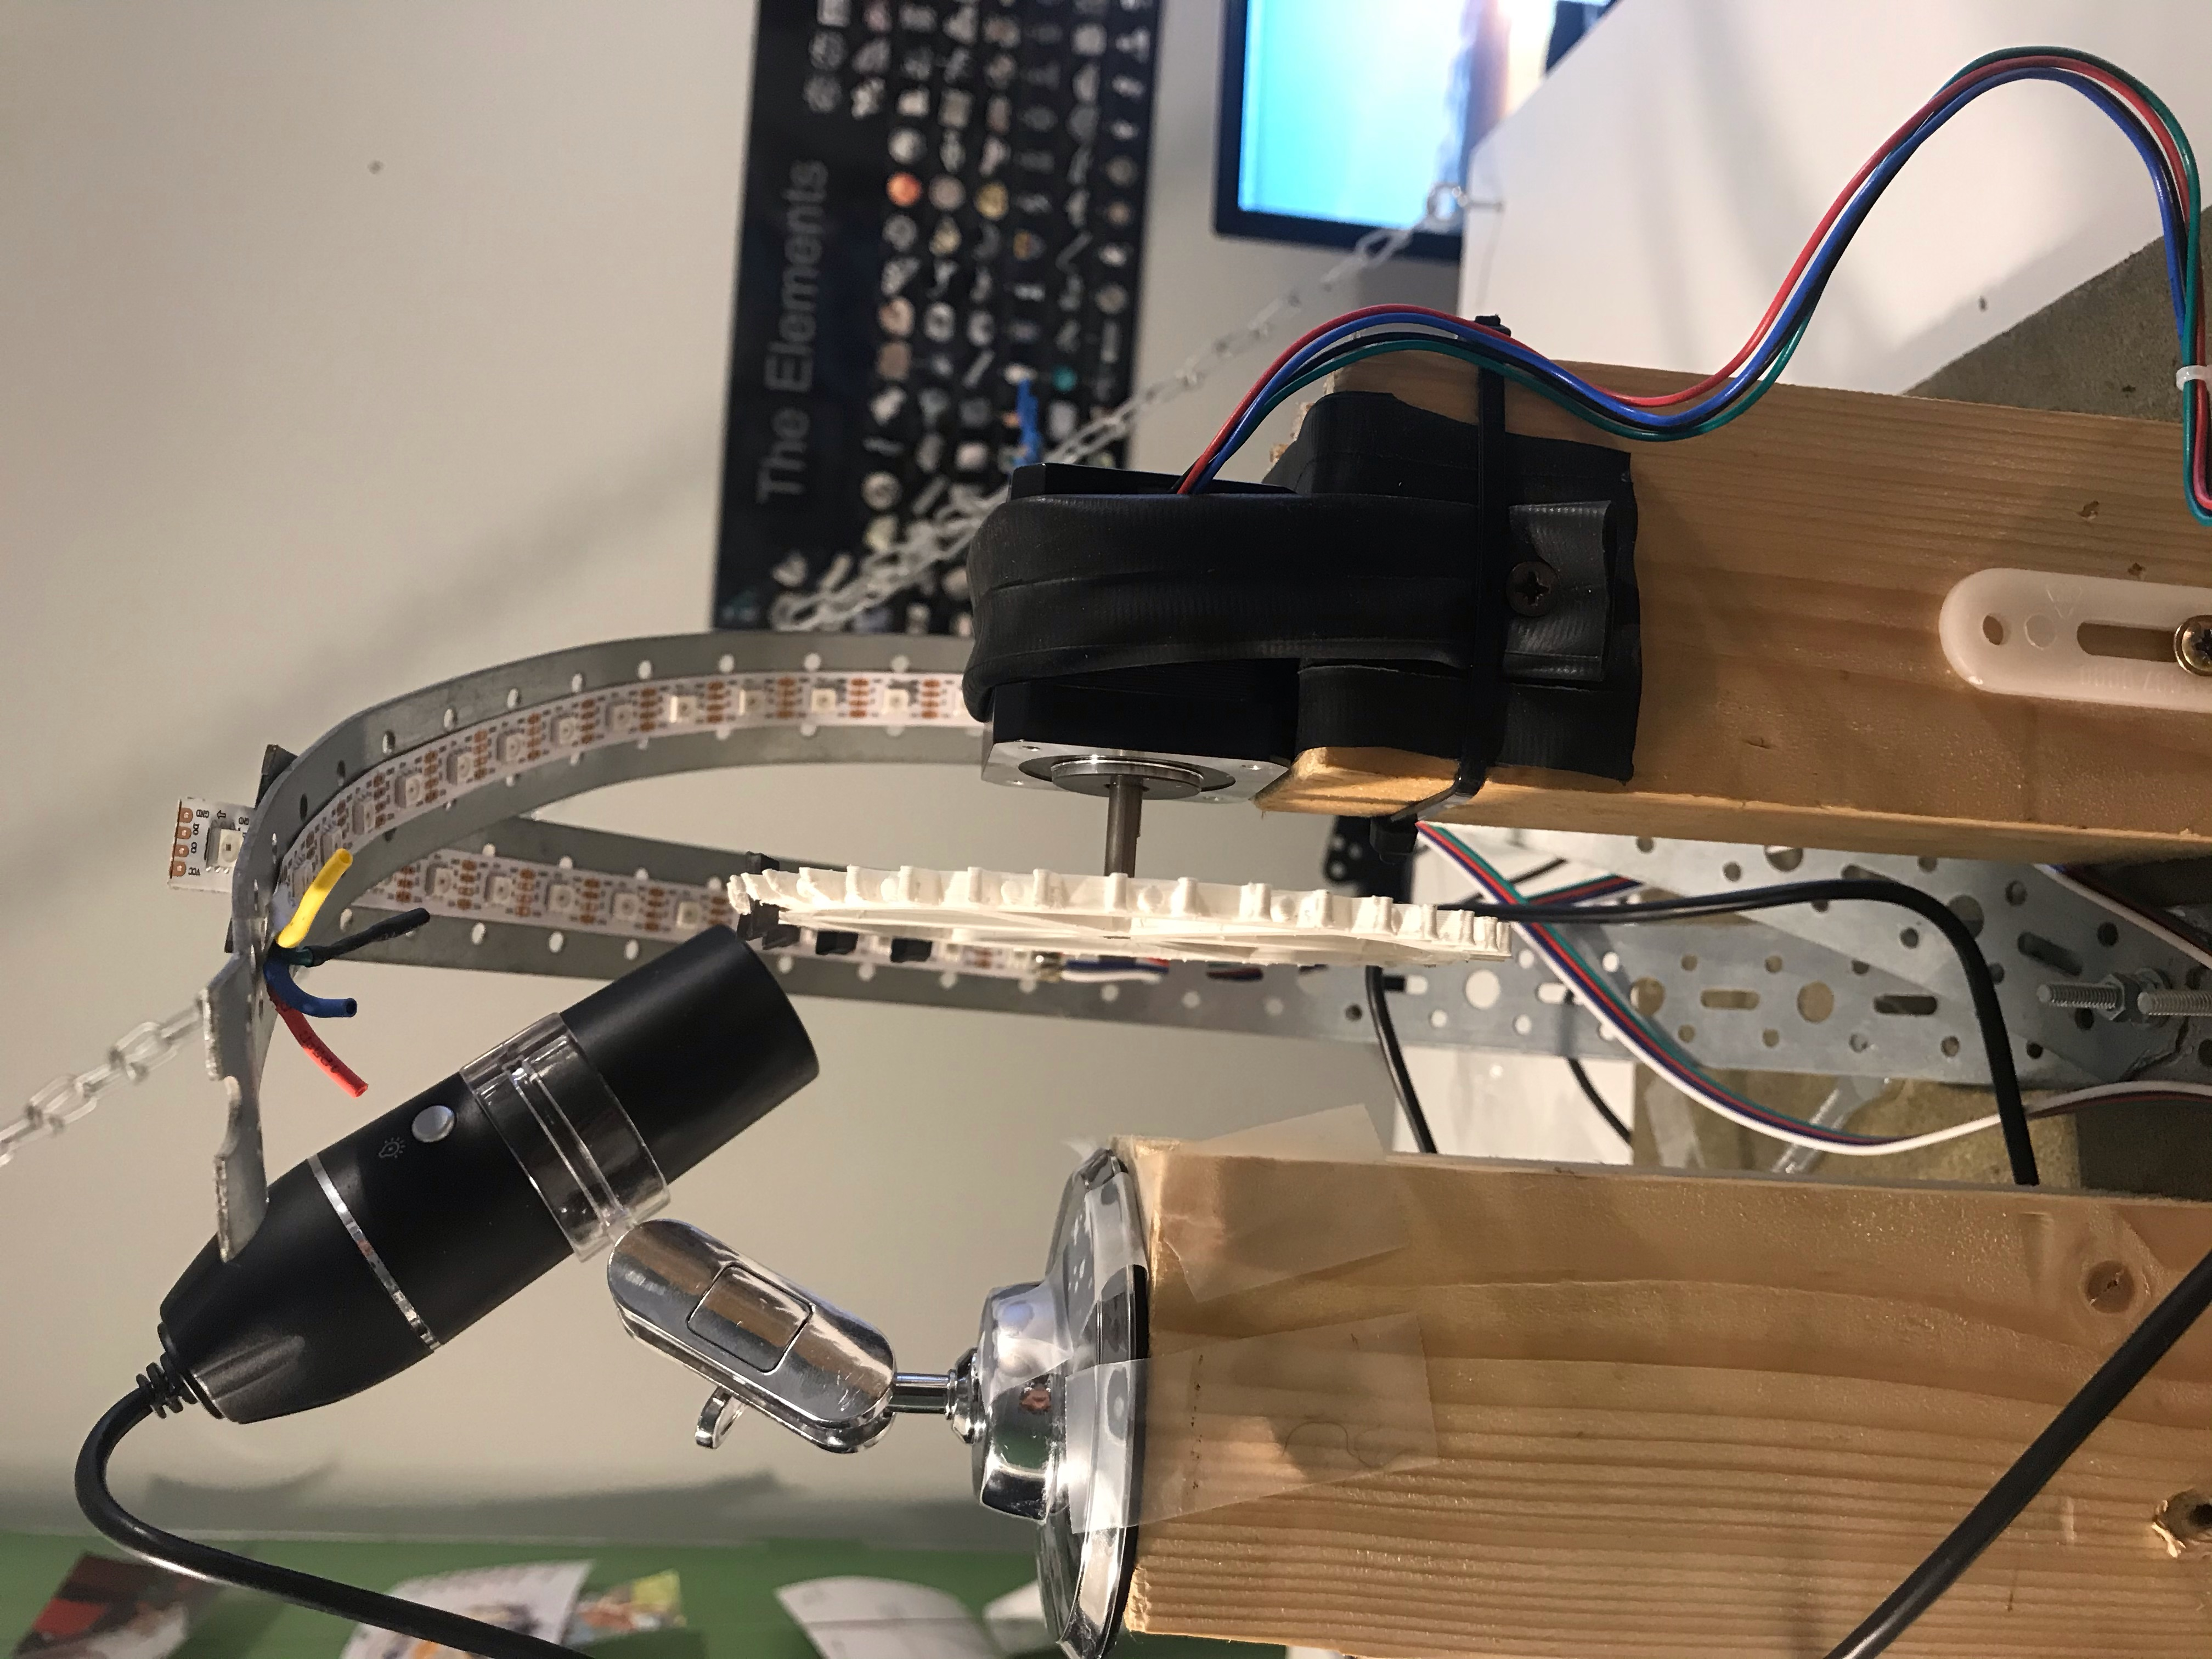
\includegraphics[width=4.166667in, keepaspectratio=true]{./ZimFiles_files/Vision/Dataset/automated_datasets/1_check_camera_position/1_camera_position_side/achter2.jpeg}



The images that where taken with this setup are found here:

Due to the problems with the arduino communications described here the first dataset wasn't successfull because the leds didn't turn on when the photo's where taken. So the results are all black pictures with al little shadow of the insert caused by the polluting light. 




\includegraphics[width=4.166667in, keepaspectratio=true]{./ZimFiles_files/Vision/Dataset/automated_datasets/1_check_camera_position/1_camera_position_side/p3_l6_black.png}



\subsection{Camera position on the side take two}



A delay was entered before sending a command to the arduino to provide the wanted lighting conditions. Although this was a very long process the results are way better than the ones from the first take on this camera setup. 



The same setup was used with the camera in the same position. For red led only the following image is the result.



The leds shown here leds 8 through 10. There is a nice lighting of every part of the wear

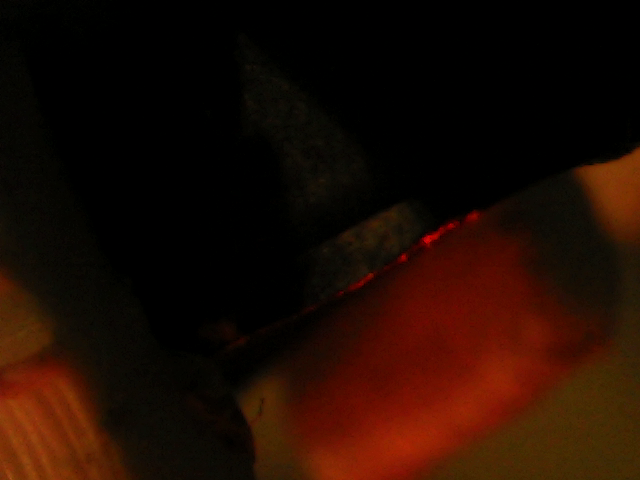
\includegraphics[width=3.125000in, keepaspectratio=true]{./ZimFiles_files/Vision/Dataset/automated_datasets/1_check_camera_position/1_camera_position_side/p3_l8.png}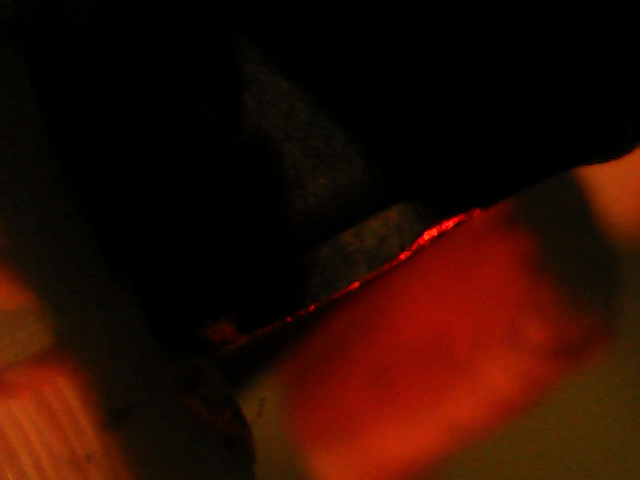
\includegraphics[width=3.125000in, keepaspectratio=true]{./ZimFiles_files/Vision/Dataset/automated_datasets/1_check_camera_position/1_camera_position_side/p3_l9.png}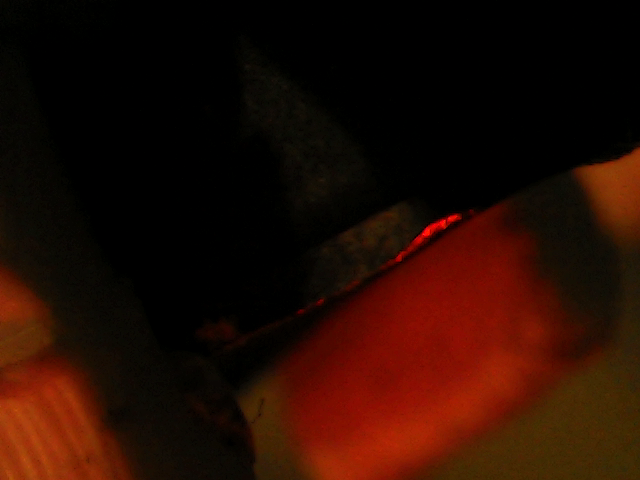
\includegraphics[width=3.125000in, keepaspectratio=true]{./ZimFiles_files/Vision/Dataset/automated_datasets/1_check_camera_position/1_camera_position_side/p3_l10.png}



This lightens the worn area very good. Although th ebackground is lighted as well and makes it harder to only see the worn area. On this we can build the first dataset. 

Next the top view was tested 


		\section{2 camera position top}

Created woensdag 11 november 2020



The same plates where used 04 -\textgreater{} 1until 5. 

Every pair of led is lighted separately to generate the photo's 



extra documents of the results in the folders images/dataset/.....



\subsection{Camera position to top}

The second test was conducted with the camera mounted a little more to the top of the inserts. This made the reflection from the worn area to the camera better. 

The first test results where also all black pictures caused by the same problem as on the first test of camera position side. On a second test this issue was resolved and the following pictures where the result. The issue was resolved by adding enormous amounts of delay for each command sent to the arduino. This made the process take very long (about 1 second per photo).



One picture was taken for every two leds of the strip with red light. for batch number 4 insert 3 with leds 5,6 and 7 turned on.



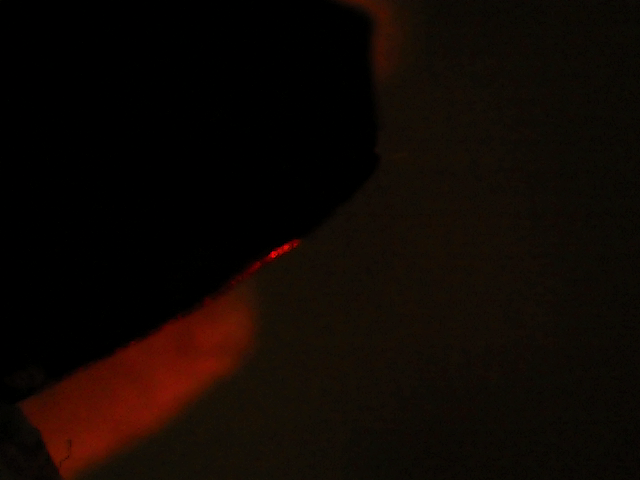
\includegraphics[width=3.125000in, keepaspectratio=true]{./ZimFiles_files/Vision/Dataset/automated_datasets/1_check_camera_position/2_camera_position_top/p3_l5.png}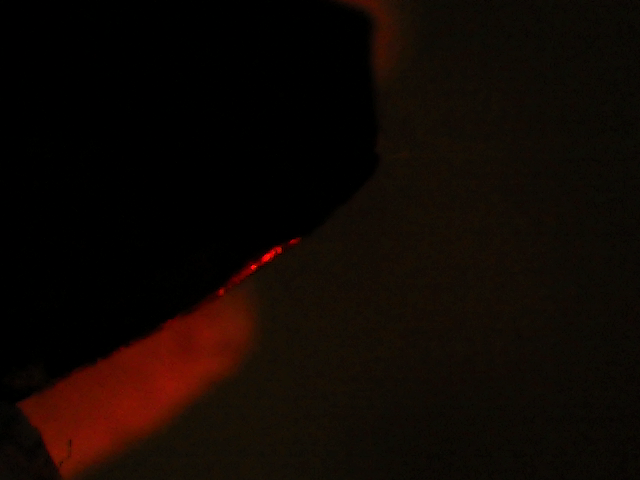
\includegraphics[width=3.125000in, keepaspectratio=true]{./ZimFiles_files/Vision/Dataset/automated_datasets/1_check_camera_position/2_camera_position_top/p3_l6.png}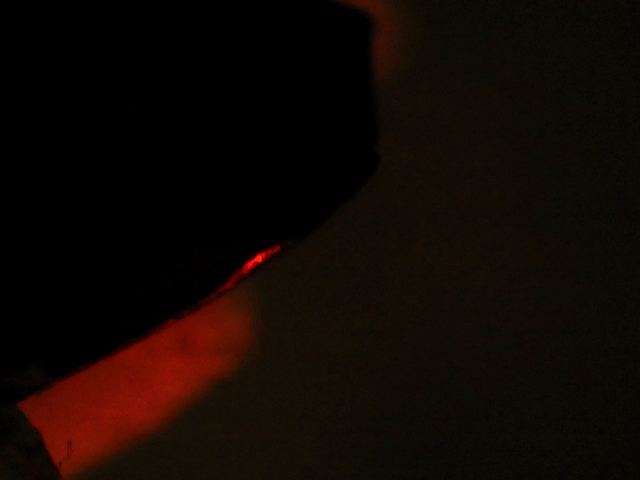
\includegraphics[width=3.125000in, keepaspectratio=true]{./ZimFiles_files/Vision/Dataset/automated_datasets/1_check_camera_position/2_camera_position_top/p3_l7.png}

On this data we can see the leds going up on the insert wear area. Which is what we tried to obtain. Now the leds are mapped to specific positions on the inserts and the amount of leds that need to be turned on for taking pictures can be reduced so no extra time is wasted. 




		\section{2 created datasets}

Created vrijdag 04 december 2020



The full datasets will be discussed in this page where firstly the dataset is documented and after that the tests that lead to this dataset are discussed.



\subsection{Birthday dataset}

Created a dataset on 27/11/2020 with a part of the given inserts for every possible color and led setting where pictures are taken from two separate led strips and every led one after another. This is done for white, red, green and blue colors. 

Done for batch 1 to 11





\subsection{spaghetti dataset}


		\section{1 Birthday dataset}

Created woensdag 02 december 2020





On November 27th a new dataset is created where for every plate 91 pictures are taken. 



The next pictures are available for the dataset:

\begin{itemize}
\item 1 picture with all leds on white
\item 30 pictures with red lighting; 15 of led strip A and 15 of led strip B
\item 30 pictures with blue lighting; 15 of led strip A and 15 of led strip B
\item 30 pictures with green lighting; 15 of led strip A and 15 of led strip B
\end{itemize}


The brightness is set to 80\% for all lights to make sure to not clip against the top values.



The dataset consists of 120*91 photos of 60 inserts with 120 worn sides. After 120 the quality was evaluated and the red, green and blue colors didn't seem to add more information to the pictures. 



In this dataset, there are some pictures unusable. As some worn areas are not even in the frame. Some to the left side and some to the right side. The placement of the wheel which holds the plates wasn't checkt thoroughly.

Picture 1: batch 3 insert 10 the side without bullet is off to the right side 

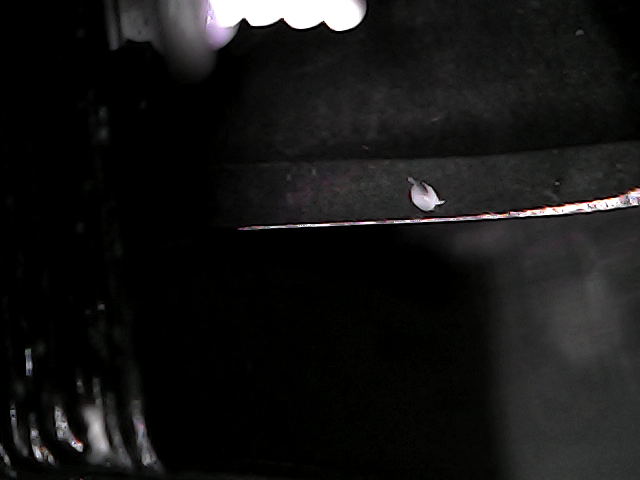
\includegraphics[width=4.166667in, keepaspectratio=true]{./ZimFiles_files/Vision/Dataset/automated_datasets/2_created_datasets/1_Birthday_dataset/b_003_p_010_l_000_nb.png}

picture 2: batch 3 insert 10 The side with bullet. Is far off to the left side.

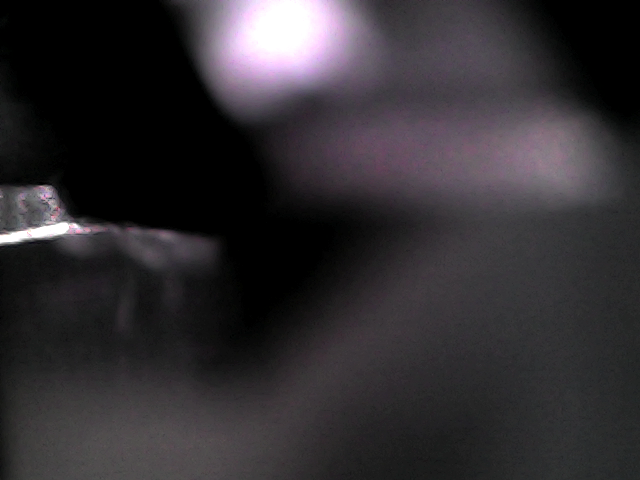
\includegraphics[width=4.166667in, keepaspectratio=true]{./ZimFiles_files/Vision/Dataset/automated_datasets/2_created_datasets/1_Birthday_dataset/b_003_p_010_l_000_b.png}



The setup for creating this dataset was as follows:

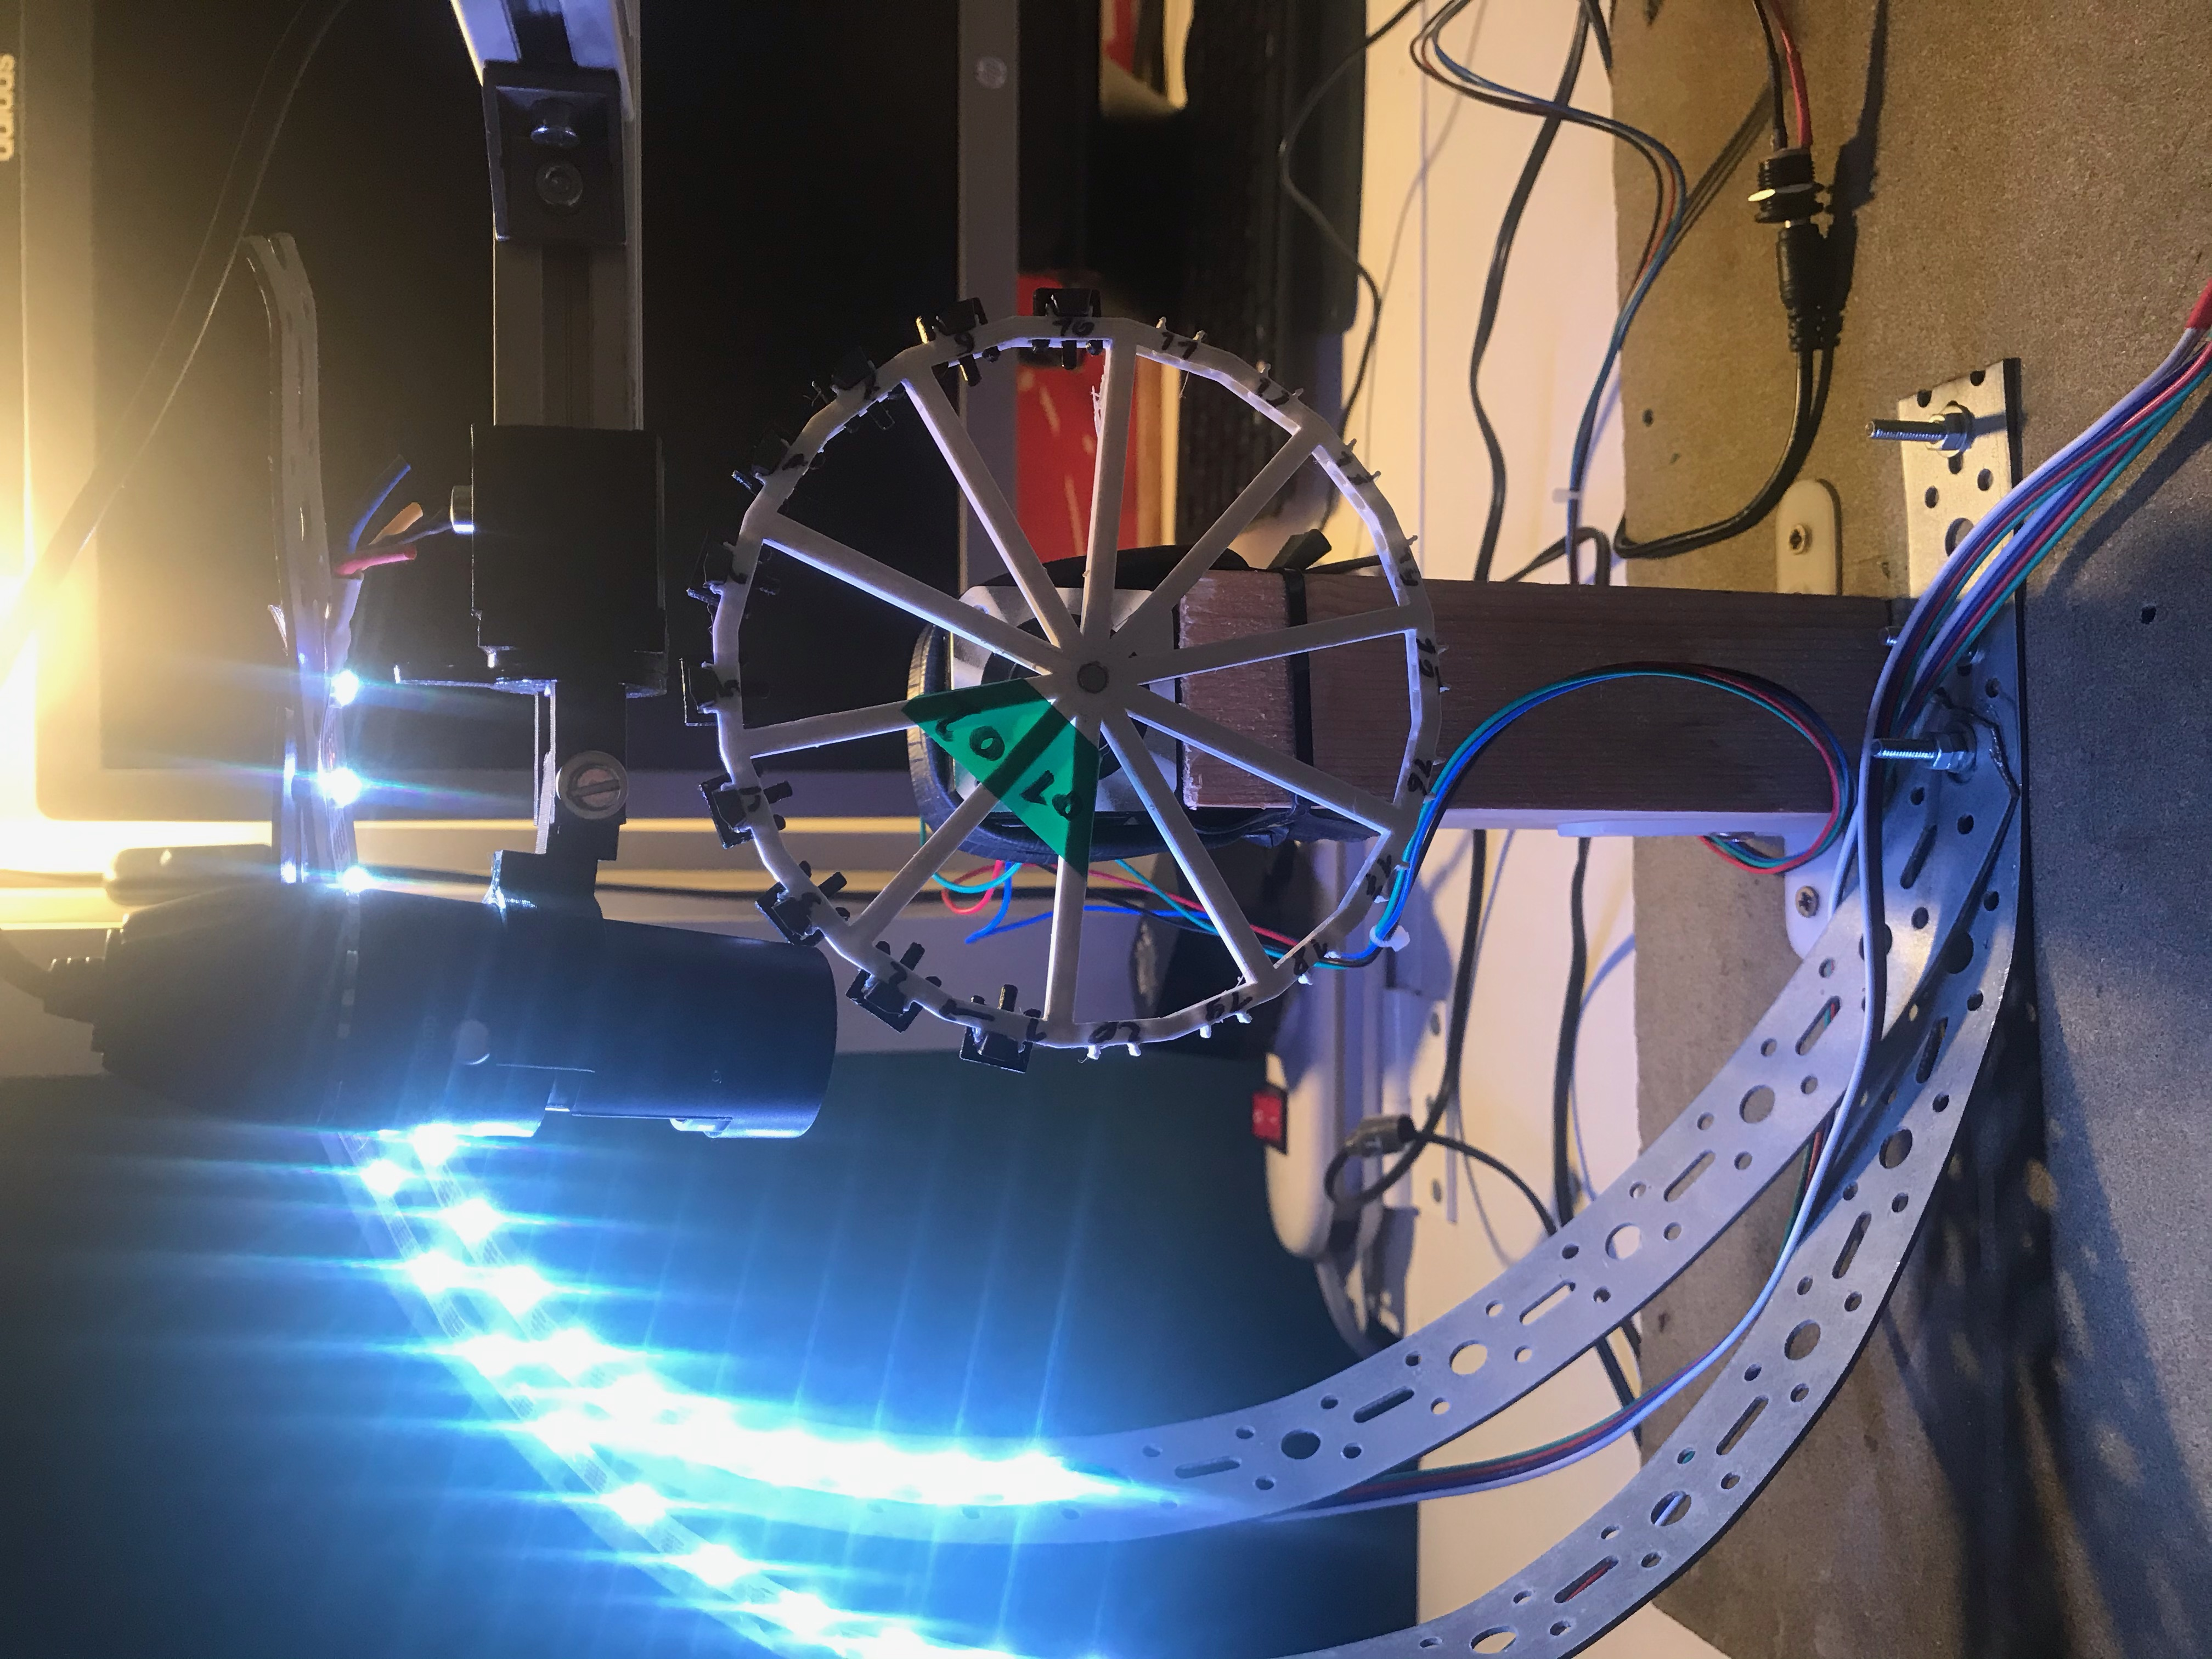
\includegraphics[width=4.166667in, keepaspectratio=true]{./ZimFiles_files/Vision/Dataset/automated_datasets/2_created_datasets/1_Birthday_dataset/IMG_9282.jpeg}

Here two ledstrips where mounted and pointed at the photographed insert. The inserts where attached to the wheel with black clips 3D printed with PETG. This was shosen above white clips to lower the light reflections into the camera lens. This was a problem in previous setups. 

Also a sturdy camera mount was fabricated out off metal profiles and 3D printed parts to get better notice of the placement of the camera opposed to the insert. 

The image taking process took about 1 minute per batch because of the amount of pictures taken. Since time was limited and the setup wasn't yet perfect we decided to only run 60 inserts through it. These where from batches 1 to 11. 

Sample pictures of this dataset can be found underneath. 

For every led one picture is taken. These images can be put together to create images on a full spectrum of leds and take out the best conditions. 

This can be done by inserting the images as different channels in the model.



The next pictures are from batch 3 insert 5 with led 6 turned on for both led strips and four colors.


\includegraphics[width=3.125000in, keepaspectratio=true]{./ZimFiles_files/Vision/Dataset/automated_datasets/2_created_datasets/1_Birthday_dataset/b_003_p_005_b_l_006_blue_A.png}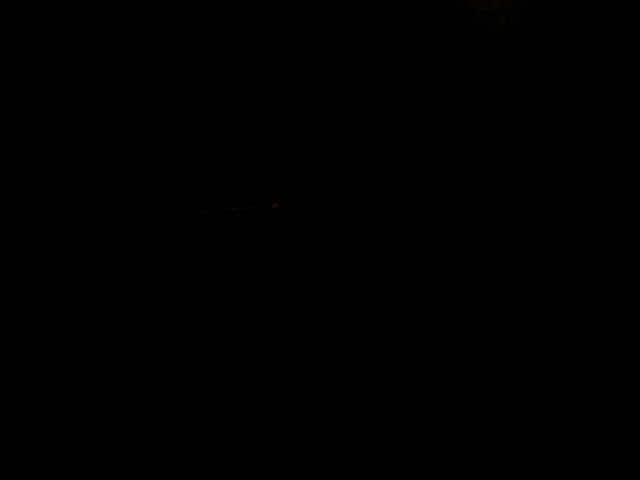
\includegraphics[width=3.125000in, keepaspectratio=true]{./ZimFiles_files/Vision/Dataset/automated_datasets/2_created_datasets/1_Birthday_dataset/b_003_p_005_b_l_006_red_A.png}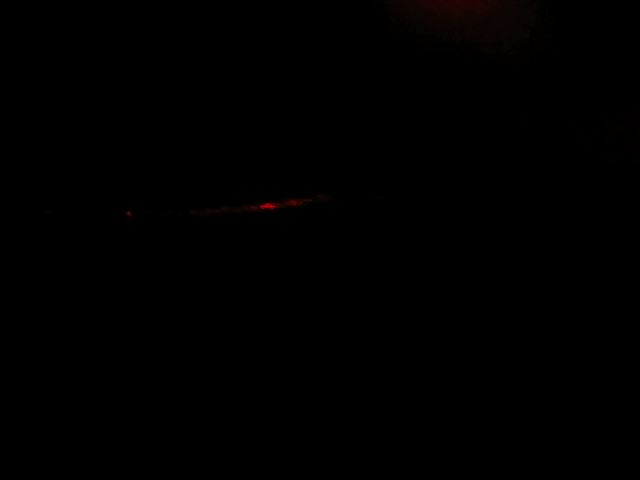
\includegraphics[width=3.125000in, keepaspectratio=true]{./ZimFiles_files/Vision/Dataset/automated_datasets/2_created_datasets/1_Birthday_dataset/b_003_p_005_b_l_006_red_B.png}
\includegraphics[width=3.125000in, keepaspectratio=true]{./ZimFiles_files/Vision/Dataset/automated_datasets/2_created_datasets/1_Birthday_dataset/b_003_p_005_b_l_006_green_A.png}
\includegraphics[width=3.125000in, keepaspectratio=true]{./ZimFiles_files/Vision/Dataset/automated_datasets/2_created_datasets/1_Birthday_dataset/b_003_p_005_b_l_006_green_B.png}\includegraphics[width=3.125000in, keepaspectratio=true]{./ZimFiles_files/Vision/Dataset/automated_datasets/2_created_datasets/1_Birthday_dataset/b_003_p_005_b_l_006_blue_B.png}\includegraphics[width=3.125000in, keepaspectratio=true]{./ZimFiles_files/Vision/Dataset/automated_datasets/2_created_datasets/1_Birthday_dataset/b_003_p_005_b_l_006_white_B.png}\includegraphics[width=3.125000in, keepaspectratio=true]{./ZimFiles_files/Vision/Dataset/automated_datasets/2_created_datasets/1_Birthday_dataset/b_003_p_005_b_l_006_white_A.png}\includegraphics[width=3.125000in, keepaspectratio=true]{./ZimFiles_files/Vision/Dataset/automated_datasets/2_created_datasets/1_Birthday_dataset/b_003_p_005_l_000_b.png}

On these pictures we can see only red and white are visible and the B led strip wasn't visible. For this purpose the color of the wheel is changed to Black for less reflections. In the next dataset only white and red will be used for lighting. 



\subsection{Code}

The code used to process this data can be found in 


		\section{conducted tests before creation}

Created vrijdag 27 november 2020



Getting first full dataset with images of all plates



\subsection{First test}

first pictures formatted with 

b\_xxx\_p\_xxx\_l\_xxx.png

	-\textgreater{} these images where from last time checking some setups
	
	



\subsection{Second test}

formatting 

next pictures without changing for different led strips

b\_xxx\_p\_xxx\_color\_l\_xxx.png



\subsection{Third test}

formatting

pictures with full experiments on lid lighting

b\_xxx\_p\_xxx\_color\_strip\_l\_xxx\_bullet.png

a video is taken here 

Here we can see a difference with or without light in the room



reformatted last images to be able to see difference between different leds, bet setup and runs are the same

b\_xxx\_p\_xxx\_bullet\_l\_xxx\_color\_strip.png





possibly 3 and 4 no bullet wrong 

rest went okay just check the batches 3 and 4



\subsection{Birthday dataset}

batch 3 plate 7 no bullet:  had restants of 3D print plastic on worn area

batch 3 plate 8 no bullet:  is a bit off picture

from here in batch 3 plates go out of sight for no bullet side. 



bullet side is going the other way out of sight for batch 3 

batch four starts of with bad pictures (also b on the left out of sight and nb on the right side out of sight



from batch 4 plate 7 it is okay again



batch 5 plate 6 no bullet lighting not good

batch 5 plate 6 bullet has string from 3D printing on wear area



batch 11 plate 5 bullet had hair on wear area


		\section{2 Spaghetti dataset}

Created vrijdag 04 december 2020



After the Birthday dataset a new dataset was created using the things learned from that. Now the amount of leds driven is reduced to 5 leds. Where led 6 to 11 is used to lighten the inserts. 

only the colors white and red are used for this dataset. This was discussed thad the red color could have an influence on the reflection of the carbide of which the inserts are made see light reflection.



\subsection{Dataset explanation}

For every insert, two pictures are taken. One with leds 6 to 11 on red and one with these leds white. This was experimentally found to be the best setting for reflecting the light off the worn area and into the camera. 

Turning on a led to much on the upper bounary will lighten the side of the insert which isn't of much use in this paper. Turining on a led to much on the bottom boundary makes the background very bright which supports unnessesary information.



The images are separated in a folder for every insert named with batch number and insert number:

batch\_aaa\_plate\_bbb where aaa is the batch number and bbb is the insert number.

Images are named with their settings, batch number and insert number:

b\_aaa\_p\_bbb\_l\_006-011\_color\_bullet.png 

where 

\begin{itemize}
\item aaa is the batch number; 
\item bbb is the plate number, 
\item 006-011 are the leds that turned on at the same time; 
\item color is the color: red or white
\item bullet is the appearance of a bullet on the side of the inset and has values of b for bullet or nb for no bullet.
\end{itemize}


The dataset inserts consisted of a few different types and coatings. 



\subsection{Setup}

The setup used is exactly the same as on the Birthday dataset where the camera is positioned as much to the top as possible. This can be seen on the picture:

Here we can see the led strips are a little bit twisted and are positioned very close to each other. This made the reflection better and should result in beter outcome of the algorithm.



\includegraphics[width=4.166667in, keepaspectratio=true]{./ZimFiles_files/Vision/Dataset/automated_datasets/2_created_datasets/2_Spaghetti_dataset/IMG_9295.jpeg}



The camera angle is kept the same a little to the top and very close to the inserts as seen on the next picture:

\includegraphics[width=4.166667in, keepaspectratio=true]{./ZimFiles_files/Vision/Dataset/automated_datasets/2_created_datasets/2_Spaghetti_dataset/IMG_9296.jpeg}



Through the whole dataset the direct light coming from other sources eg. the light of the room was blocked to have full control of the lighting conditions.



\subsection{Results}

Underneath are some pictures of good examples in the dataset.



Underneath are two pictures of batch 3 insert 6. These where lid with red light on the left and white light on the right. Here is a nice wear shown and lighted. However if we zoom in to the picture the top part of the wear is not lighted that well. We can also see a white piece of the insert holder on the image which is providing som extra difficulties. The discussion of these difficulties will be bespoken in vision algorithm.

\includegraphics[width=3.125000in, keepaspectratio=true]{./ZimFiles_files/Vision/Dataset/automated_datasets/2_created_datasets/2_Spaghetti_dataset/b_003_p_006_l_006-011_red_nb.png}\includegraphics[width=3.125000in, keepaspectratio=true]{./ZimFiles_files/Vision/Dataset/automated_datasets/2_created_datasets/2_Spaghetti_dataset/b_003_p_006_l_006-011_white_nb.png}



Some pictures aren't sharp like the one shown next.

like batch 5 insert 5 withoud bullet.

\includegraphics[width=3.125000in, keepaspectratio=true]{./ZimFiles_files/Vision/Dataset/automated_datasets/2_created_datasets/2_Spaghetti_dataset/b_005_p_005_l_006-011_white_nb.png}



\paragraph{Different insert types}

First type are the grey inserts with very visible wear. These are seen in batches 1 to 5 consistently. This type will be called grey inserts.

\includegraphics[width=3.125000in, keepaspectratio=true]{./ZimFiles_files/Vision/Dataset/automated_datasets/2_created_datasets/2_Spaghetti_dataset/gray_b_003_p_004_l_006-011_white_nb.png}



Than there are other inserts in batch 11 which are also grey but have a different shape on the cutting part. These will be called rounded grey inserts.

\includegraphics[width=3.125000in, keepaspectratio=true]{./ZimFiles_files/Vision/Dataset/automated_datasets/2_created_datasets/2_Spaghetti_dataset/rounded_grey_b_011_p_008_l_006-011_white_nb.png}

In batch 12 and 13 there are the same shape of inserts but with a black coating which results in way darker pictures as seen here on batch 13 insert 2 no bullet. These inserts are the rounded black inserts.

\includegraphics[width=3.125000in, keepaspectratio=true]{./ZimFiles_files/Vision/Dataset/automated_datasets/2_created_datasets/2_Spaghetti_dataset/rounded_black_b_013_p_002_l_006-011_white_nb.png}



The next type are copper colored inserts with the rounded shape. Seen in batch 14 insert 5 no bullet.

\includegraphics[width=3.125000in, keepaspectratio=true]{./ZimFiles_files/Vision/Dataset/automated_datasets/2_created_datasets/2_Spaghetti_dataset/rounded_copper_b_014_p_005_l_006-011_white_nb.png}



Than we have inserts with a gold coating and hooked shape. For batch 15 insert 6 no bullet that gives the next picture:

\includegraphics[width=3.125000in, keepaspectratio=true]{./ZimFiles_files/Vision/Dataset/automated_datasets/2_created_datasets/2_Spaghetti_dataset/rounded_gold_b_015_p_006_l_006-011_white_nb.png}




































		\section{camera position}

Created woensdag 11 november 2020



1st test was with a camera position more to the side of the cutting plates. This resulted in a bad reflection angle since the light came from the wrong side. Documentation of this set is in automated datasets:1 check camera position:1 camera position side


		\section{handmade datasets}

Created vrijdag 04 december 2020




		\section{initial dataset}

Created vrijdag 13 november 2020



\subsection{Form}

The dataset given where taken with a microscopic camera at Sirris. These images were in good lighting conditions for the measurement, but had a lot of extra "unwanted" features on it. The background was very like the wear and the rest of the tool insert. 

Every insert that was measured had a little mark on one side to mark the a and b. Sadly the information about what the marker meant is lost. To find the corresponding values, the inserts where once again put through a microscopic camera and the new pictures where compared against the old ones. 



While again checking the inserts out, a new dataset is created since this didn't ask much more time. During this proces there is also a new way of separating the sides of the inserts. There is a bullet at one side on every insert. This is an easy way to recognise a side and wont dissapear like the marker line. 







\includegraphics[width=3.125000in, keepaspectratio=true]{./ZimFiles_files/Vision/Dataset/handmade_datasets/initial_dataset/initial dataset pictuer.PNG}




		\section{Second handmade dataset}

Created vrijdag 13 november 2020



A second handmade dataset is made to compare with the first dataset and get to know what the stripes mean on the first dataset which was used to measure the wear.



The next setup is used:

The light came primarely from the camera itself which was set in the first brightness setting. 

The camera was located at a distance of 2cm between the housing and the measured point on the insert. The housing starts at the black part; not the plexi glass protector. 

During the making of this dataset the inserts where labeled with bullet or no bullet. This was not setup this way in the first place; instead there was a marker line on the insert. This marker line is also noted in the labels of the dataset.

An "s" means it is with a marker line. A

\begin{tabular}{ |l|l| }
\hline
 symbol & explanation \tabularnewline
\hline
\hline
 s & side with marker line \tabularnewline
\hline
 n & side without marker line \tabularnewline
\hline
 batch number & number specified on the box in which the inserts are kept \tabularnewline
\hline
 plate number & number specified inside the box; this goes from 1 to 10 per batch \tabularnewline
\hline
\end{tabular}


The naming of the dataset is the following

b\_\textless{}batch number\textgreater{}\_p\_\textless{}plate number\textgreater{}\_\textless{}identifier of side\textgreater{}

After looking at the pictures of the datasets it can be confirmed that the 'b' side of the inserts is the side with the mark on. 



This can be seen on the folowing two pictures whis correspond. The first one is from the first dataset, the second from the second dataset.

\includegraphics[height=2.083333in, keepaspectratio=true]{./ZimFiles_files/Vision/Dataset/handmade_datasets/Second_handmade_dataset/t50b-img.PNG}\includegraphics[height=2.083333in, keepaspectratio=true]{./ZimFiles_files/Vision/Dataset/handmade_datasets/Second_handmade_dataset/b_005_p_010_s.jpg}


		\section{second initial dataset}

Created vrijdag 04 december 2020



With the second number of inserts (batch 11 to 19) another dataset was created for measurement.

Since the photo's where labeled with two inserts at a time; the images taken where not relevant for the data processing and were not saved



The distance for these inserts is measured between the line connecting the two highest points visible on the insert and the outer most point of the wear area.






		\section{GoogleColab}

Created woensdag 04 november 2020




		\section{Test Camera Setup}

Created woensdag 04 november 2020



To test the camera setup, a binary classification model is made. This model will tell with a treshold of 150 (200 the real treshold but 150 to warn before tool is worn out) wether a tool is good to work with or must be removed from the machine. 

This model should be trainable with as less images as possible, preferably 20 because that is the amount of pictures taken in one batch.





\subsection{Resnet18}

First we will try to implement SDD-Resnet18 to classify the few images in good or bad. 



\subsection{nception v3}

Than we will implement SDD-inception v3 



These described models should perform rather good without any transfer learning. 

After the first tests these results can be compared with a transfer learning model.





\subsection{All Networks}

For this all networks test, some networks where tested and an algorithm is created to make it possible to add more networks along the way


		\section{All Networks}

Created woensdag 02 december 2020




		\section{All Networks 1}

Created woensdag 02 december 2020



All networks 1 can be found \href{https://colab.research.google.com/drive/1bWt0DgypiYoOOgnSGjlmSdDo7elvJnH4}{here.}



\subsection{Network architectures}

This model is used to test different model architectures namely:

\begin{itemize}
\item Resnet18
\item Alexnet
\item VGG11\_bn
\item Squeezenet
\item Densenet
\end{itemize}


inception v3 didn't seem to work



These models are all relatively small and should provide quite good results for a small dataset. 

More on why the models should work can be found here



\subsection{Dataset}



This algorithm had the input of images from the Second handmade dataset which was devided into 3 classes based on their measured wear value. 

\begin{tabular}{ |l|l|l| }
\hline
 class & min value (micron) & max value (micron) \tabularnewline
\hline
\hline
 good & 0 & 130 \tabularnewline
\hline
 medium & 130 & 230 \tabularnewline
\hline
 bad & 230 & ∞ \tabularnewline
\hline
\end{tabular}










\subsection{Results}

Results of this notebook are available on wandb as \href{https://wandb.ai/dplars/pytorch-TWI_second_handmade?workspace=user-dplars}{pytorch-TWI\_second\_handmade}



Interesting results will be bespoken here;

Tests for different models: 

\begin{tabular}{ |l|l|l|l| }
\hline
 model name & test accuracy \% & validation accuracy\% & transfer learning \tabularnewline
\hline
\hline
 Alexnet & 100 & 90 & yes \tabularnewline
\hline
 VGG11\_bn & 89 & 85 & yes \tabularnewline
\hline
 Densenet & 89 & 85 & yes \tabularnewline
\hline
 Squeezenet & 89 & 85 & yes \tabularnewline
\hline
 Resnet18 & 89 & 90 & no \tabularnewline
\hline
\end{tabular}
										

An overview of the best runs for every model architecture. Since there are only nine test images; the test scores are set to a very high granularity. Further results of this test are to be found on wandb as \href{https://wandb.ai/dplars/pytorch-TWI_second_handmade/reports/Testing-on-first-handmade-dataset--VmlldzozNTE5NzM}{Testing on first handmade dataset}


		\section{All Networks 2}

Created vrijdag 04 december 2020



\subsection{Network architectures}

This model is used to test different model architectures namely:

\begin{itemize}
\item Resnet18
\item Alexnet
\item VGG11\_bn
\item Squeezenet
\item Densenet
\end{itemize}


inception v3 didn't seem to work



These models are all relatively small and should provide quite good results for a small dataset. 

More on why the models should work can be found here



\subsection{Dataset}



This algorithm had the input of images from the Second handmade dataset which was devided into 3 classes based on their measured wear value. 

\begin{tabular}{ |l|l|l| }
\hline
 class & min value (micron) & max value (micron) \tabularnewline
\hline
\hline
 good & 0 & 130 \tabularnewline
\hline
 medium & 130 & 230 \tabularnewline
\hline
 bad & 230 & ∞ \tabularnewline
\hline
\end{tabular}










\subsection{Results}

Results of this notebook are available on wandb as \href{https://wandb.ai/dplars/pytorch-TWI_second_handmade?workspace=user-dplars}{pytorch-TWI\_second\_handmade}



Interesting results will be bespoken here;

Tests for different models: 

\begin{tabular}{ |l|l|l|l| }
\hline
 model name & test accuracy \% & validation accuracy\% & transfer learning \tabularnewline
\hline
\hline
 Alexnet & 100 & 100 & yes \tabularnewline
\hline
 Resnet18 & 100 & 95 & no \tabularnewline
\hline
 Densenet & 100 & 85 & yes \tabularnewline
\hline
 Squeezenet & 100 & 85 & yes \tabularnewline
\hline
 VGG11\_bn & 100 & 90 & no \tabularnewline
\hline
\end{tabular}
										

An overview of the best runs for every model architecture. Since there are only nine test images; the test scores are set to a very high granularity. Further results of this test are to be found on wandb as \href{https://wandb.ai/dplars/pytorch-TWI_second_handmade/reports/Testing-on-first-handmade-dataset--VmlldzozNTE5NzM}{Testing on first handmade dataset}





Trying to sweep over different parameter settings didn't work on my local computer; all runs failed or crashed


		\section{All Networks 3 Birthday}

Created vrijdag 04 december 2020



The code for this project is to be found here: \href{https://colab.research.google.com/drive/1_DKPtHi231TMalsj-uaBLytjcX2DuyV4#scrollTo=vmsTN_T4xoXP}{TSU\_AllNetworks\_3\_Birthday}


		\section{All Networks 4 Spaghetti}

Created vrijdag 04 december 2020



The code for this can be found in here: \href{https://colab.research.google.com/drive/1kKCU9pAsVRqNR-lX1p45Z7BLTxp76CMq}{TSU\_AllNetworks\_4\_spaghetti}





The report is noted in \href{https://wandb.ai/dplars/pytorch-TWI_spaghetti_sweep/reports/Spaghetti-sweep-with-TSU_AllNetworks_4_spaghetti--VmlldzozNTIxNjM}{Spaghetti sweep with TSU\_AllNetworks\_4\_spaghetti} This can be transformed into latex without further problems i hope.


		\section{All networks 4 spaghetti first 5 batches}

Created vrijdag 04 december 2020



Only the first five batches are analysed in this report to check if the dataset is as good as the dataset created by hand of these batches.

Also the difference is checked between the red and white leds.




		
		\section{Resnet18}

Created woensdag 18 november 2020



In this page we will describe the results and actions taken to get results out of Resnet18



this paper suggests that this is a good architecture for a quite like problem. where a low amount of data is used.

	\emph{SDD-CNN: Small data-driven convolution neural networks for subtle roller defect inspection}
	


\subsection{Creating first file}



\subsection{TSU\_Resnet18\_1}



failed to load data, did copy files into correct directories and created dataset class



\subsection{TSU\_Resnet18\_2}



Simpeler method to read in data and not be able to change a lot of things;

next time build dataset class self with the same model. 

After that the regression model would be easy



First result of the training.

\includegraphics[height=4.166667in, keepaspectratio=true]{./ZimFiles_files/Vision/GoogleColab/Test_Camera_Setup/Resnet18/Screenshot 2020-11-18 at 22.58.45.png}

Tweede test met een aanpassing van de learning rate en een foto van de training set naar test set gebracht

\includegraphics[height=4.166667in, keepaspectratio=true]{./ZimFiles_files/Vision/GoogleColab/Test_Camera_Setup/Resnet18/Screenshot 2020-11-18 at 23.13.23.png}



Next time create results file to get nice overview of all results



\end{document}
